% !TeX root = ../../Skript.tex
\cohead{\Large\textbf{Exponentialfunktionen}}
\fakesubsection{Exponentialfunktionen}
Wir werden im Folgenden als Basis nur die eulersche Zahl \(e=2,71828\dots\) als Basis verwenden. Man kann jede Exponentialfunktion zur Basis \(e\) schreiben, indem man im Exponenten einen zusätzlichen Faktor hinzufügt, z.B. \(f(x)=10\cdot 2^x=10\cdot e^{\ln(2)\cdot x}\). Dabei ist \(\ln(2)=\log_e(2)\) der Logarithmus zur Basis \(e\). Diesen werden wir später noch genauer betrachten.

Wie die parabelförmigen und S-förmigen Schaubilder bei den ganzrationalen Funktionen, bilden die folgenden 4 Schaubilder die Grundbausteine, um Schaubilder zu skizzieren.

Die Funktion \(f(x)=a\cdot e^{k\cdot x},\ a\neq 0,\,k\neq 0\) nimmt in Abhängigkeit der Vorzeichen von \(a\) und \(k\) folgende vier Formen an:

\medskip

\begin{minipage}{\textwidth}
	\adjustbox{valign=t, padding =0ex 0ex 2ex 0ex}{\begin{minipage}{0.5\textwidth-2ex}
		\begin{minipage}{\textwidth}
			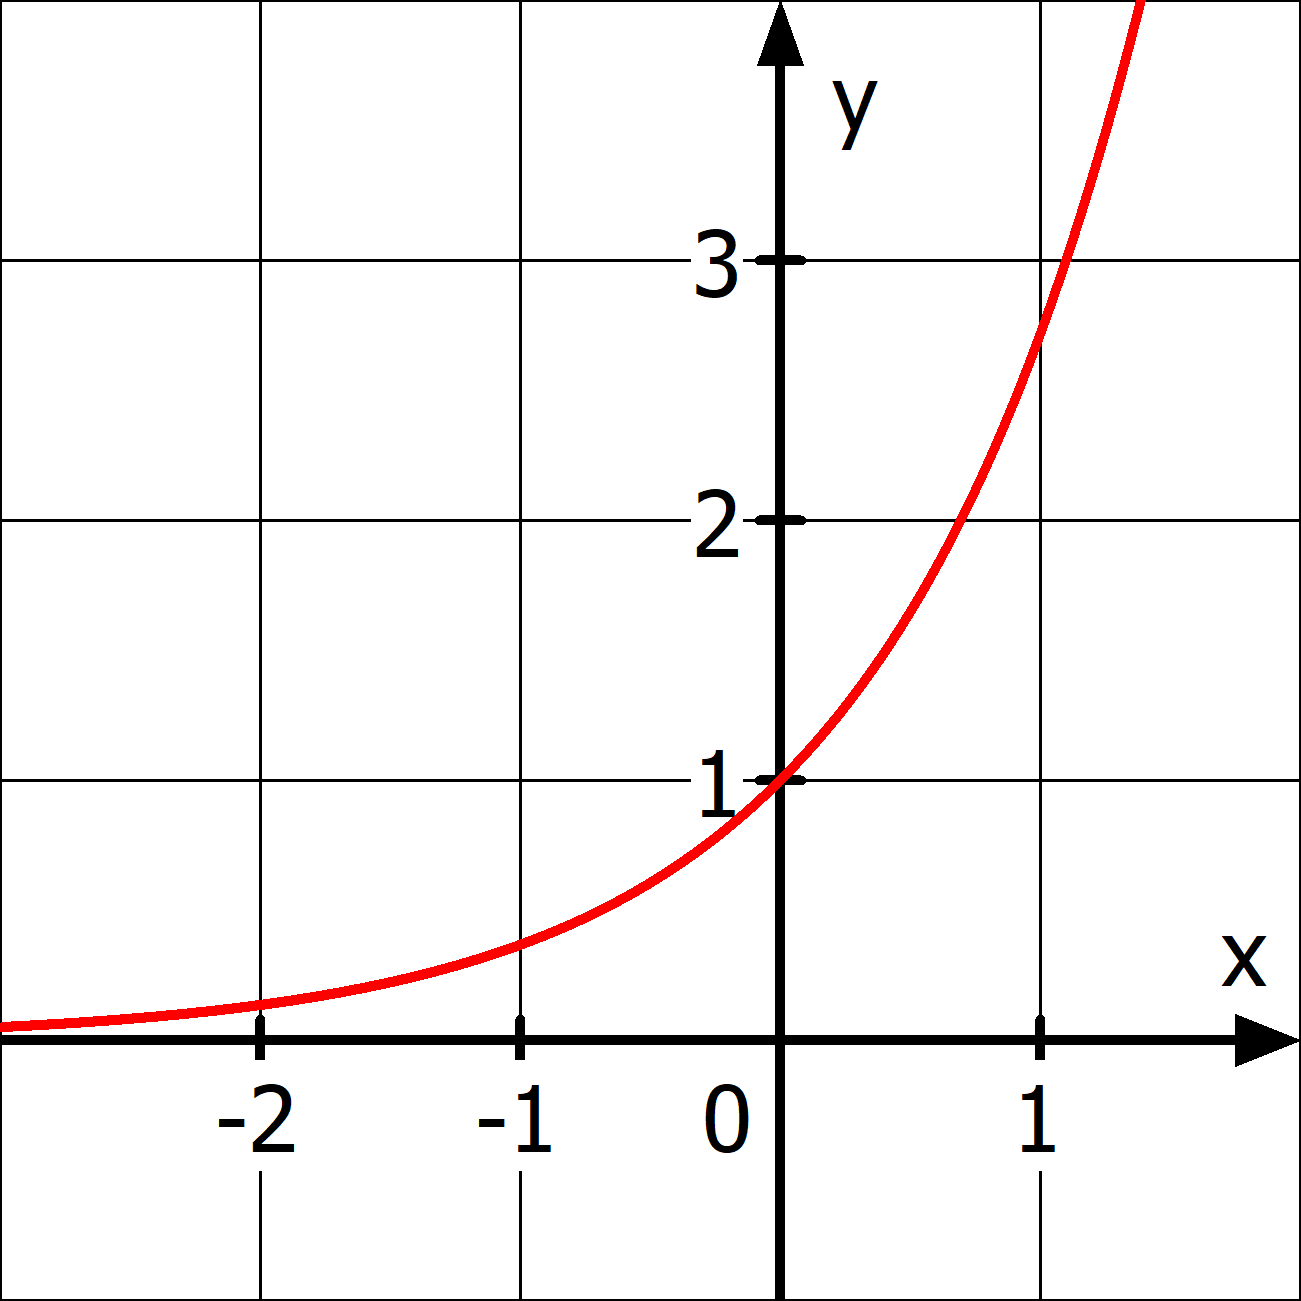
\includegraphics[width=\linewidth]{\eFkt/pics/e_x.png}
		\end{minipage}%

		\centering \(a\) positiv, \(k\) positiv, z.B. \(f_1(x)=e^x\)
	\end{minipage}}%
	\adjustbox{valign=t, padding =2ex 0ex 0ex 0ex}{\begin{minipage}{0.5\textwidth-2ex}
		\begin{minipage}{\textwidth}
			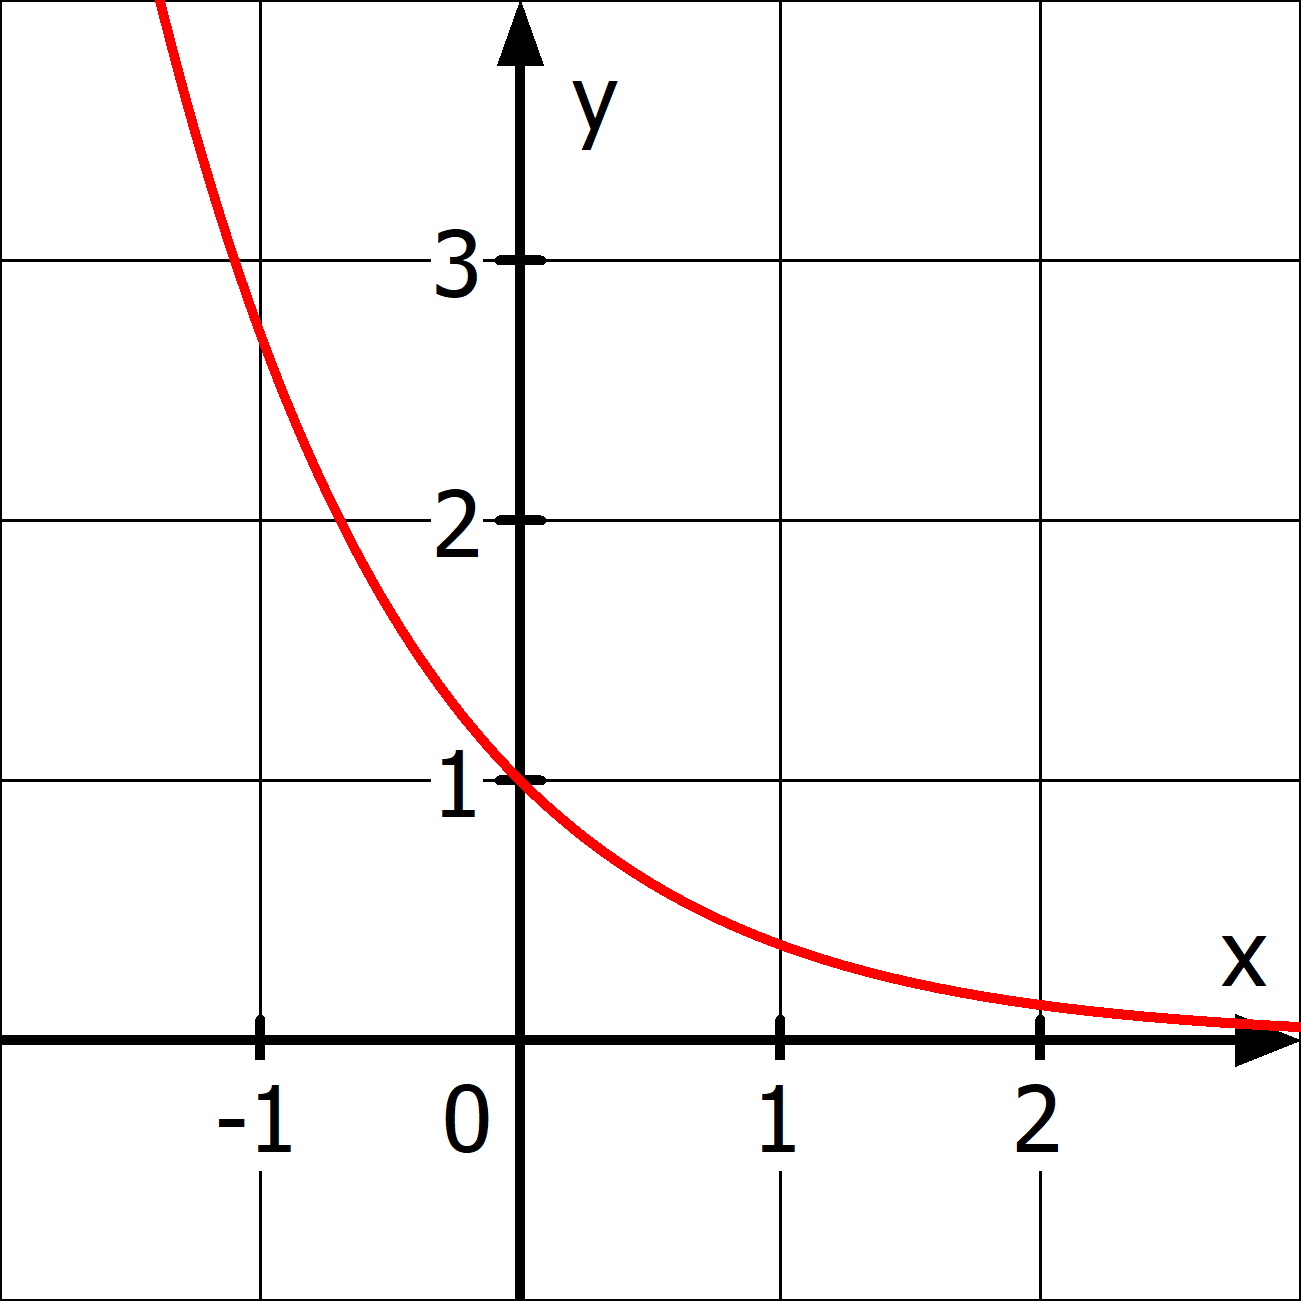
\includegraphics[width=\linewidth]{\eFkt/pics/e_minusx.png}
		\end{minipage}%

		\centering \(a\) positiv, \(k\) negativ, z.B. \(f_2(x)=e^{-x}\)
	\end{minipage}}%
\end{minipage}

\medskip

\begin{minipage}{\textwidth}
	\adjustbox{valign=t, padding =0ex 0ex 2ex 0ex}{\begin{minipage}{0.5\textwidth-2ex}
		\begin{minipage}{\textwidth}
			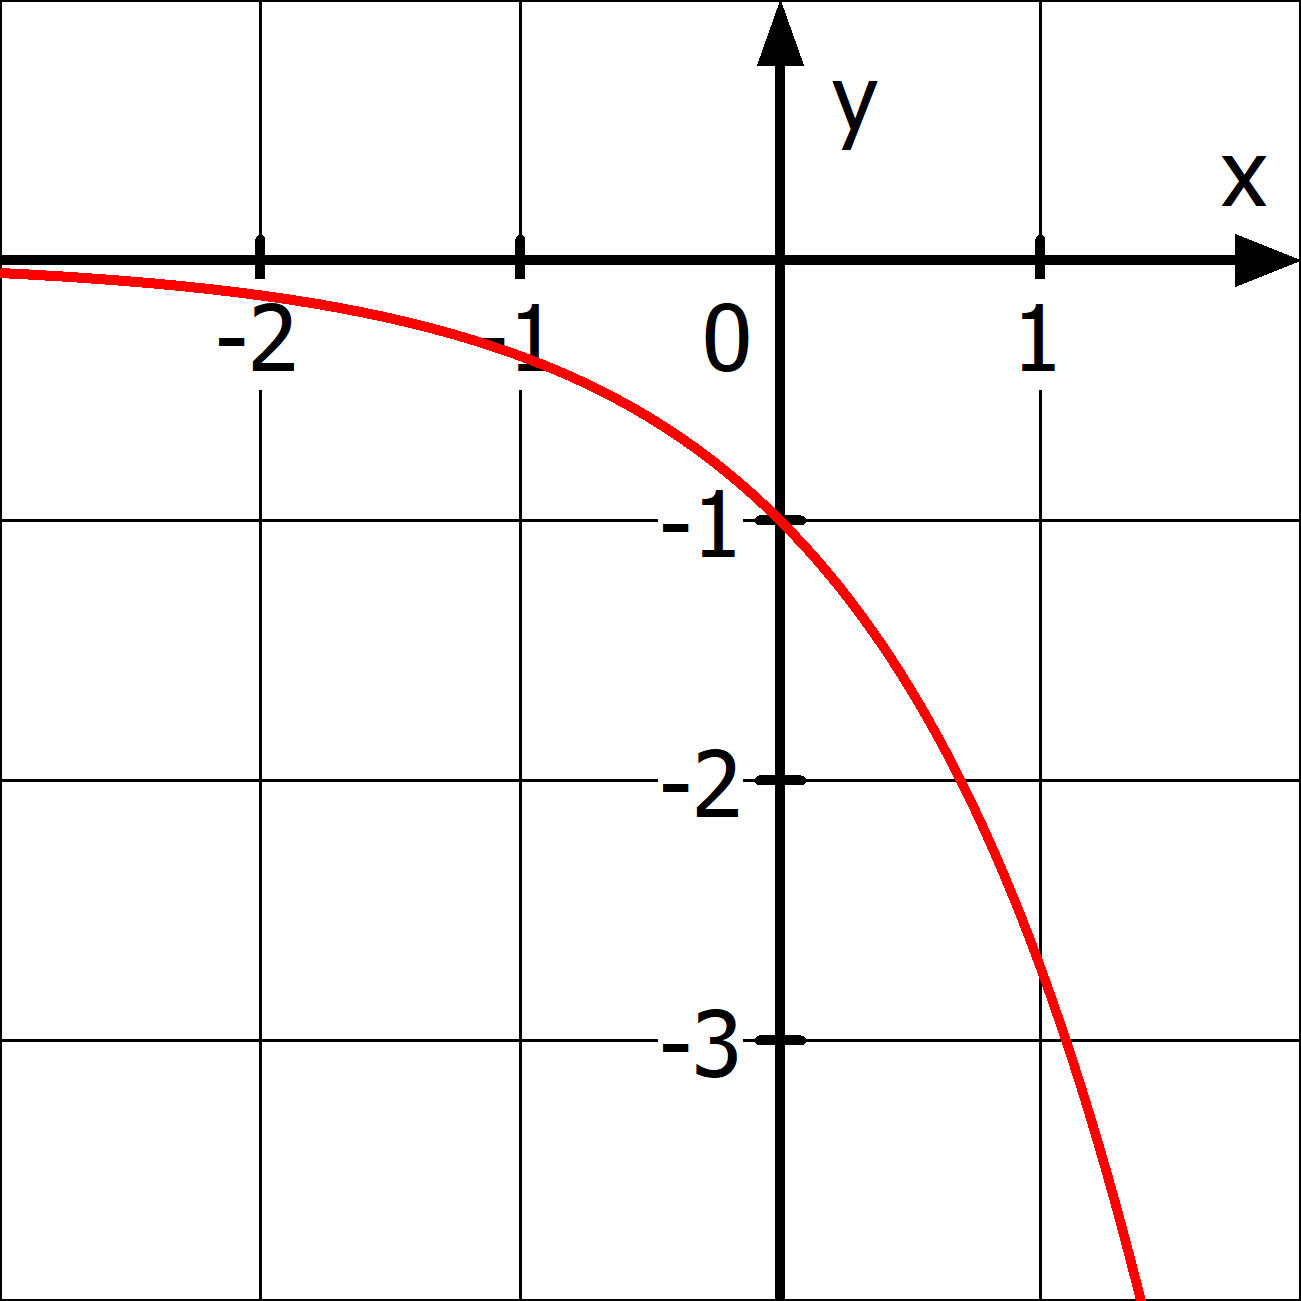
\includegraphics[width=\linewidth]{\eFkt/pics/minuse_x.png}
		\end{minipage}%

		\centering \(a\) negativ, \(k\) positiv, z.B. \(f_3(x)=-e^x\)
	\end{minipage}}%
	\adjustbox{valign=t, padding =2ex 0ex 0ex 0ex}{\begin{minipage}{0.5\textwidth-2ex}
		\begin{minipage}{\textwidth}
			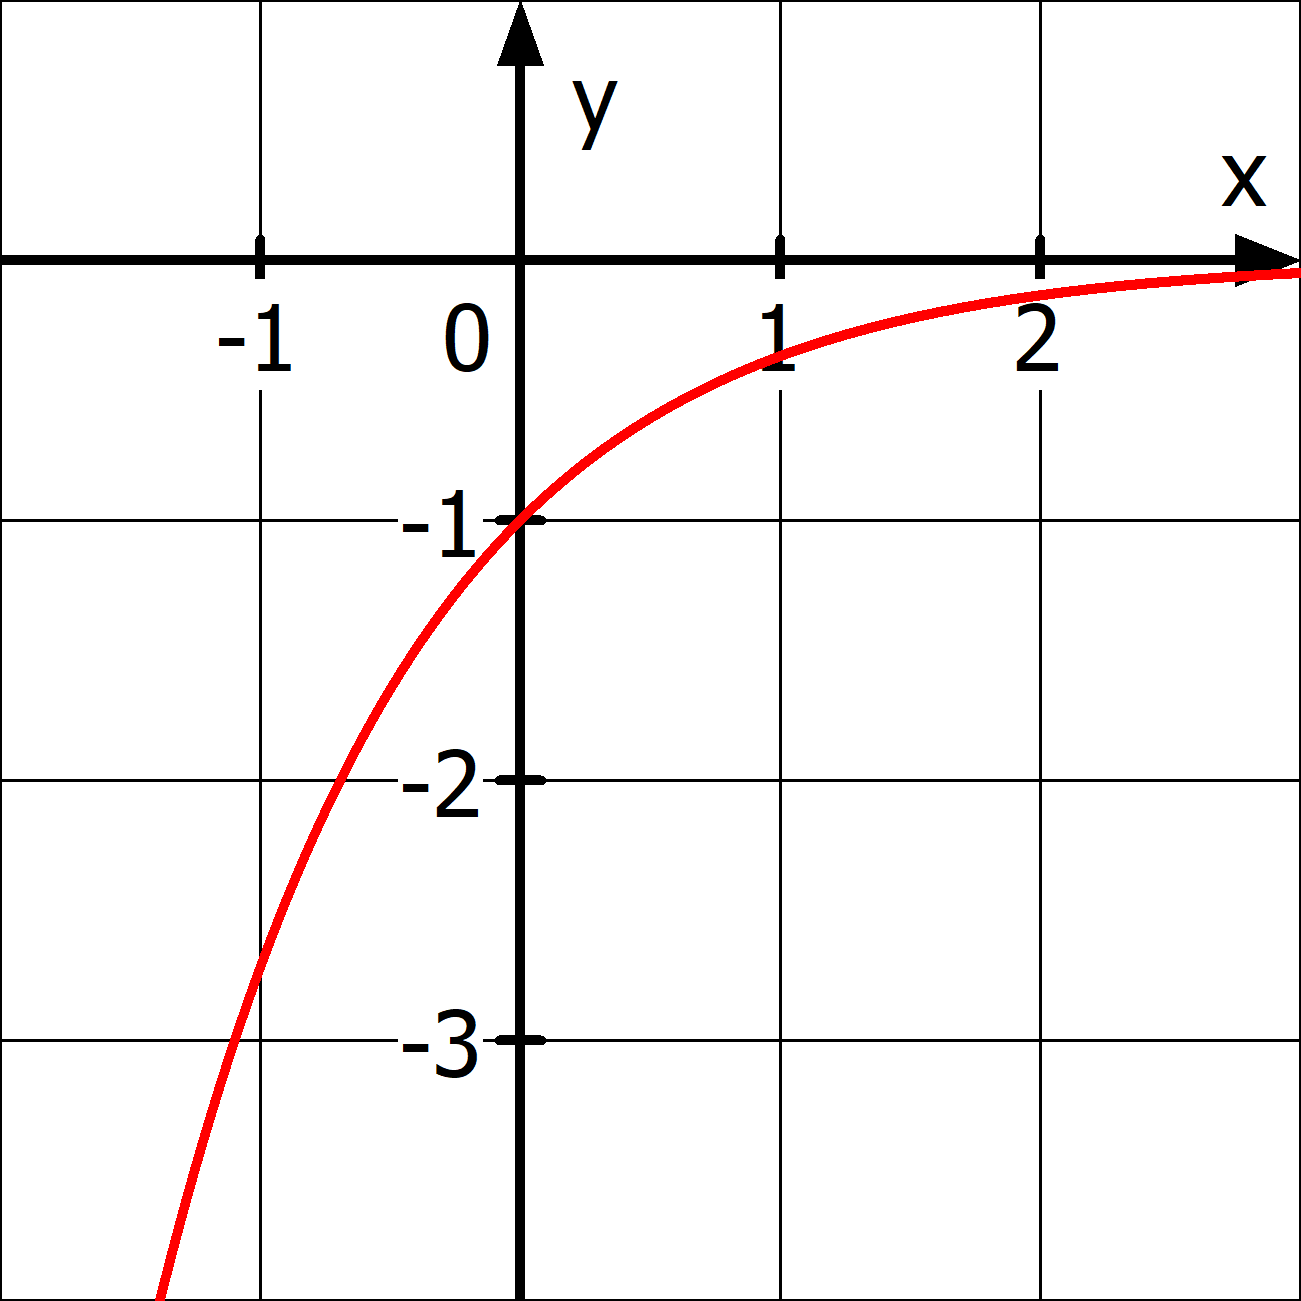
\includegraphics[width=\linewidth]{\eFkt/pics/minuse_minusx.png}
		\end{minipage}%

		\centering \(a\) negativ, \(k\) negativ, z.B. \(f_4(x)=-e^{-x}\)
	\end{minipage}}%
\end{minipage}%

\begin{tcolorbox}Wichtiger Funktionswert von \(e^x\):
	\[\bm{e^0=\textcolor{loestc}{1}}\]
\end{tcolorbox}
\newpage
%%%%%%%%%%%%%%%%%%%%%%%%%%%%%%%%%%%%%%%%%%%%%%%%%%%%%%%%%%%%%%%%%%%%%%%%%%%%%%%%%%%%%%%%%%%%%%%%%%%%%%
\cohead{\Large\textbf{Begriffe}}
Zur Einführung der neuen Begriffe Asymptote und Monotonie betrachten wir als Beispiel

\(f(x)=e^{\ln(2)\cdot x}=2^x\):

\bigskip

\begin{minipage}{\textwidth}
	\adjustbox{valign=t}{\begin{minipage}{0.55\textwidth}
		\begin{tcolorbox}
			\textbf{Asymptote}

			\textcolor{loestc}{Eine Asymptote einer Funktion ist eine Gerade, an die sich die Funktion beliebig nahe annähert, d.h. der Abstand zw. der Funktion und der Geraden wird beliebig klein. Im Beispiel halbiert man den Funktionswert immer wenn man einen Schritt nach links macht. Die Funktionswerte gehen also immer näher an die Null heran. Die Asymptote ist die x-Achse bzw. \(y=0\)}
            \vspace{3.32cm}
		\end{tcolorbox}
	\end{minipage}}%
	\adjustbox{valign=t, padding =2ex 0ex 0ex 0ex}{\begin{minipage}{0.45\textwidth-2ex}
		\begin{minipage}{\textwidth}
			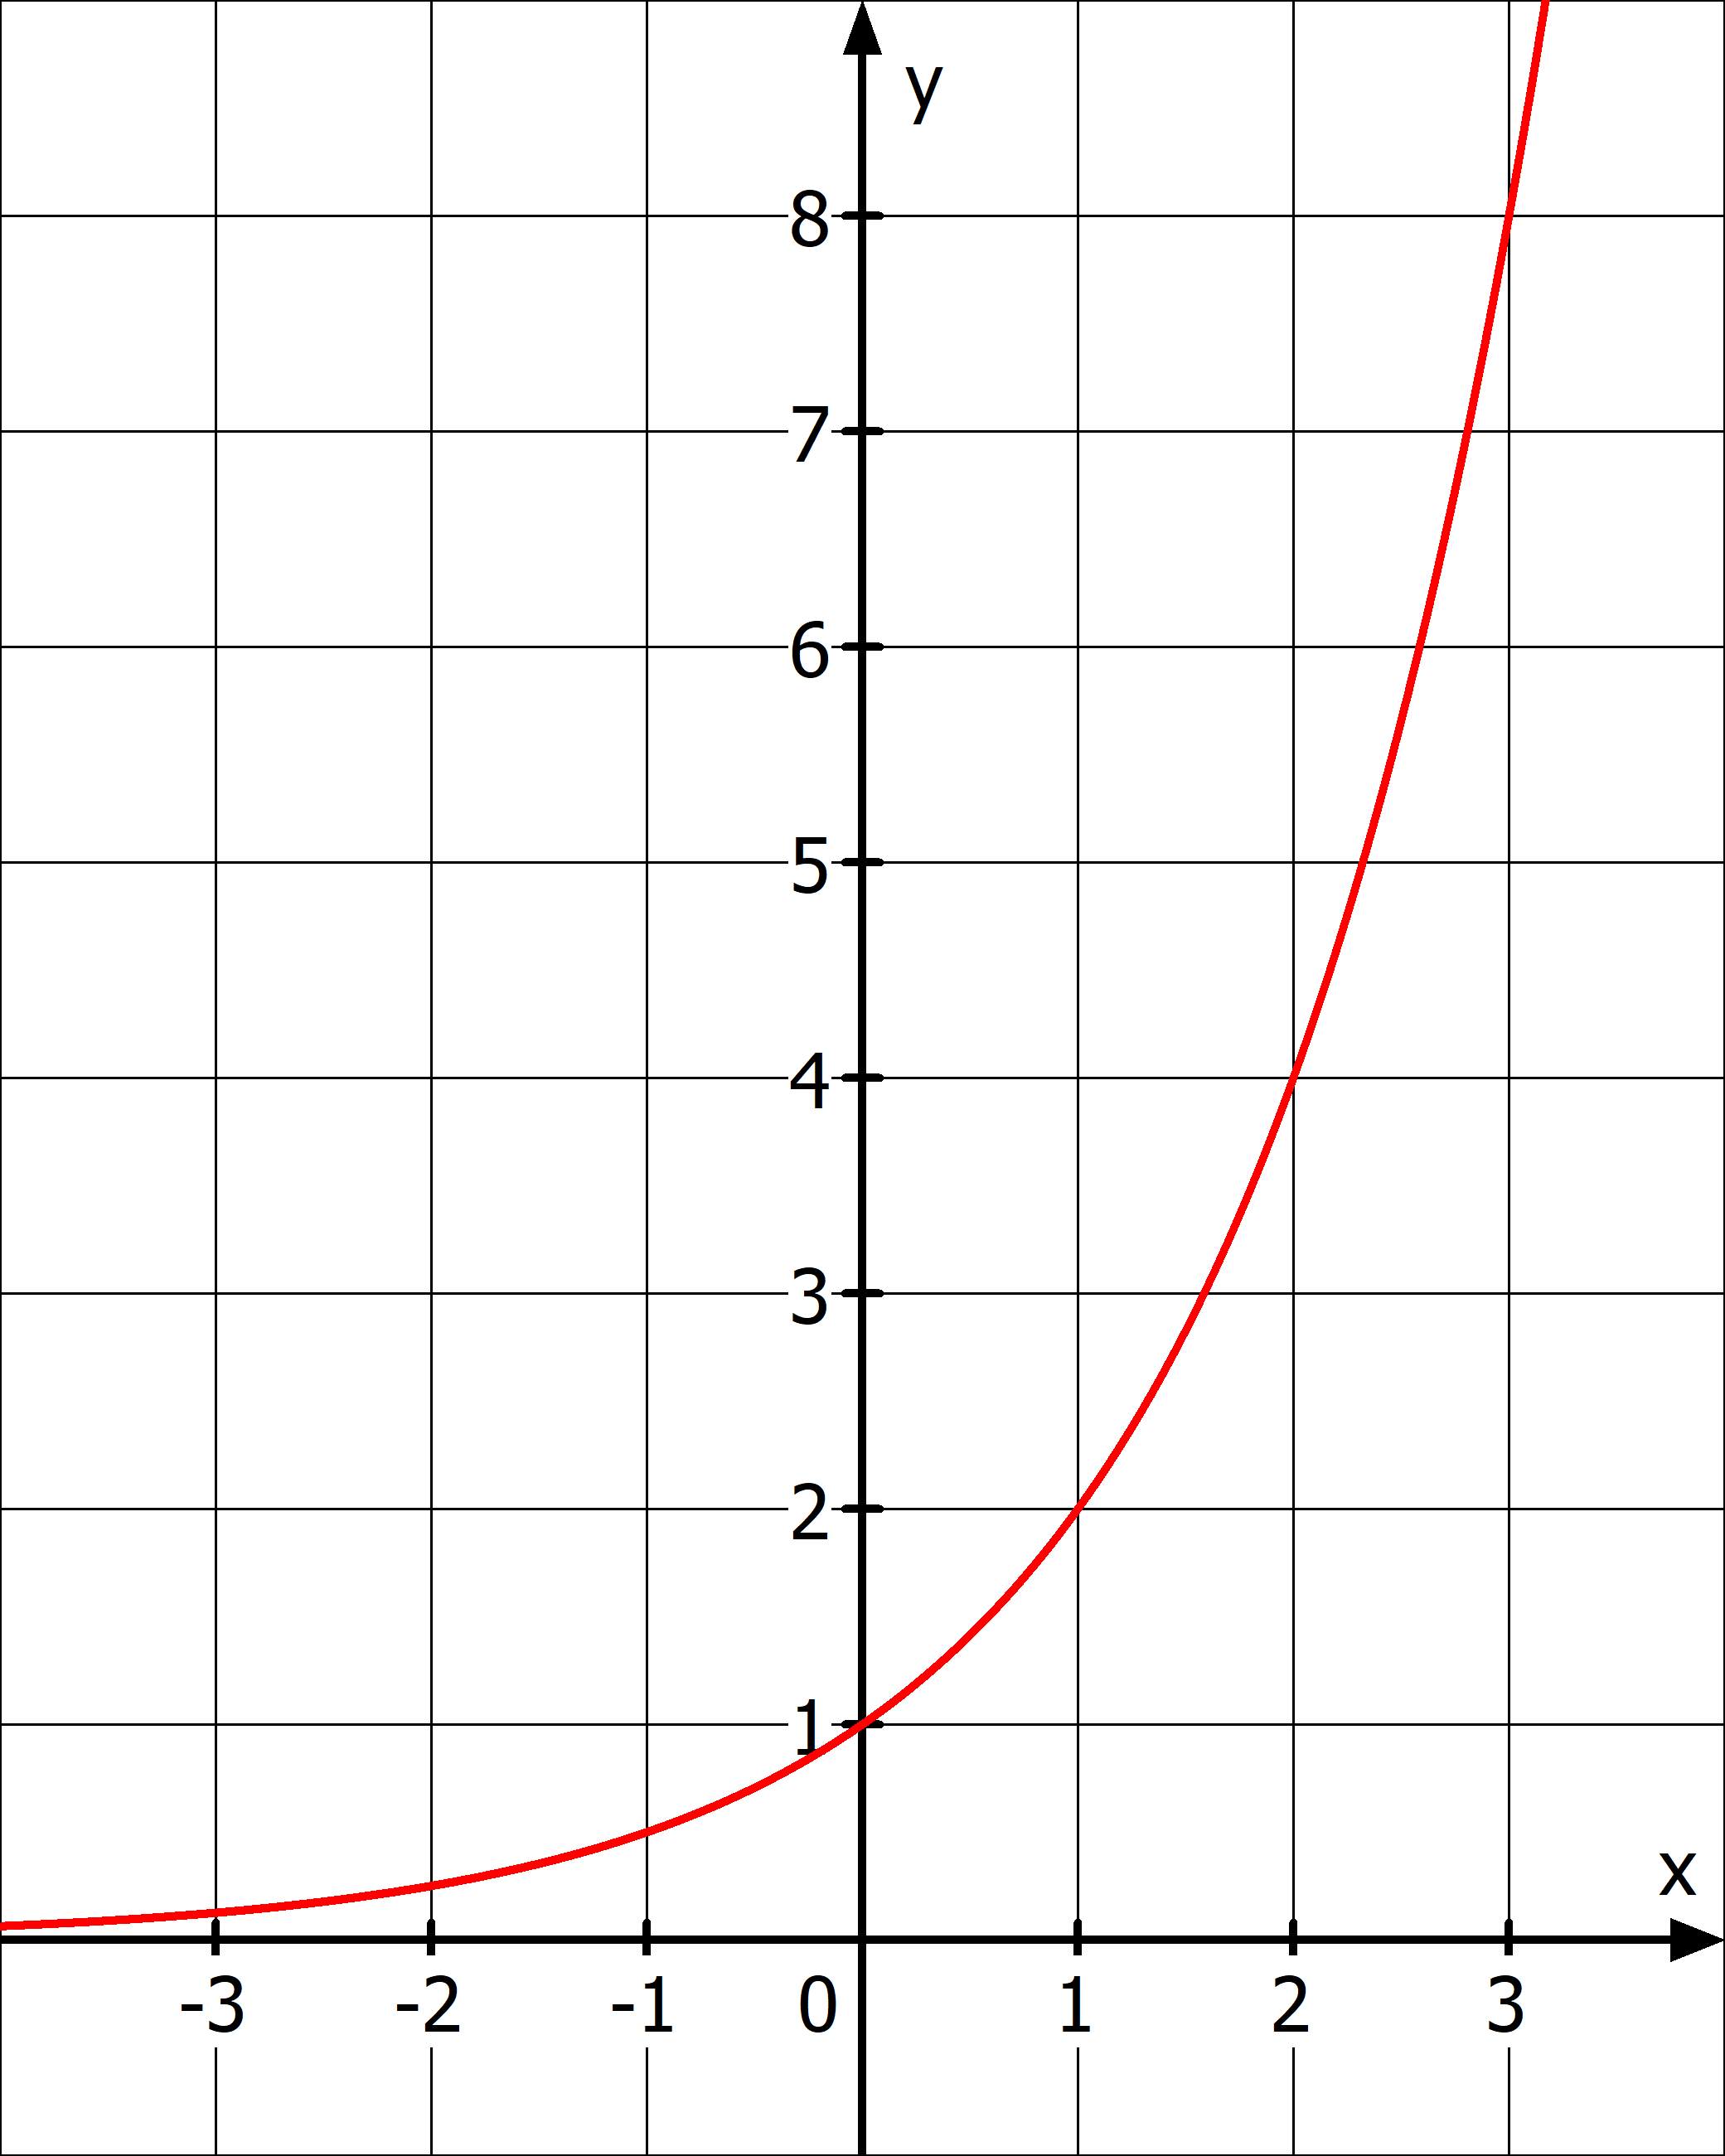
\includegraphics[width=\linewidth]{\eFkt/pics/2hochx.png}
		\end{minipage}%
	\end{minipage}}%
\end{minipage}

\medskip

\begin{tcolorbox}
	\textbf{Verhalten für \(x\rightarrow \pm\infty\)}
	\textcolor{loestc}{
		\begin{align*}
			f(x)&\xrightarrow{\hphantom{\ }x\to-\infty\hphantom{\ }}0\\
			f(x)&\xrightarrow{\hphantom{\ }x\to\infty\hphantom{\ }}\infty
	\end{align*}}
    \vspace{1cm}
\end{tcolorbox}
\begin{tcolorbox}
	\textbf{Monotonie}

	\textcolor{loestc}{Wachsen die Funkionswerte bzw. y-Werte mit wachsenden x-Werten, so ist die Funktion monoton wachsend. Werden die Funktionswerte mit wachsenden x-Werten immer kleiner, so ist die Funktion Monoton fallend.}

	\textcolor{loestc}{Das Beispiel ist also monoton wachsend, da man von links nach rechts immer weiter nach oben geht. (Die Funktionswerte verdoppeln sich mit jedem Schritt nach rechts.)\vspace{3cm}}
\end{tcolorbox}
\newpage
%%%%%%%%%%%%%%%%%%%%%%%%%%%%%%%%%%%%%%%%%%%%%%%%%%%%%%%%%%%%%%%%%%%%%%%%%%%%%%%%%%%%%%%%%%%%%%%%%%%%%%%%%%%%%%%%%%%%%
\begin{Exercise}[title={Bestimme den y-Achsenabschnitt, skizziere das Schaubild, gib die Asymptote, das Verhalten für \(x\rightarrow \pm\infty\) und die Monotonie an}, label=eFktA1]\\
	\begin{minipage}{\textwidth}
		\begin{minipage}{0.49\textwidth}
			\begin{enumerate}[label=\alph*)]
				\item \(f(x)=e^{2x}\)
				\item \(f(x)=-3e^{\frac{1}{2}x}\)
				\item \(f(x)=-4e^{-2x}\)
				\item \(f(x)=2e^{-7x}\)
				\item \(f(x)=-\frac{5}{3}e^{x}\)
				\item \(f(x)=8e^{-3x}\)
				\item \(f(x)=-3e^{-\frac{9}{8}x}\)
				\item \(f(x)=\frac{3}{5}e^{0,2x}\)
				\item \(f(x)=-0,5e^{-3,5x}\)
				\item \(f(x)=-8e^{\frac{1}{10}x}\)
				\item \(f(x)=2e^{-2x}\)
				\item \(f(x)=-4e^{-7x}\)
				\item \(f(x)=-\frac{5}{7}e^{x}\)
			\end{enumerate}
		\end{minipage}
		\begin{minipage}{0.49\textwidth}
			\begin{enumerate}[label=\alph*)]
				\setcounter{enumi}{13}
				\item \(f(x)=6e^{-4x}\)
				\item \(f(x)=-2e^{-8x}\)
				\item \(f(x)=5,3e^{0,2x}\)
				\item \(f(x)=-\frac{1}{4}e^{-\frac{2}{3}x}\)
				\item \(f(x)=-2e^{0,2x}\)
				\item \(f(x)=1,8e^{-4x}\)
				\item \(f(x)=5e^{7x}\)
				\item \(f(x)=-\frac{8}{3}e^{\frac{3}{8}x}\)
				\item \(f(x)=-0,1e^{-0,3x}\)
				\item \(f(x)=10e^{-4x}\)
				\item \(f(x)=-5e^{6x}\)
				\item \(f(x)=-0,9e^{-1,1x}\)
				\item \(f(x)=\frac{11}{6}e^{\frac{8}{7}x}\)
			\end{enumerate}
		\end{minipage}
	\end{minipage}
\end{Exercise}
\newpage
%%%%%%%%%%%%%%%%%%%%%%%%%%%%%%%%%%%%%%%%%
\begin{Answer}[ref=eFktA1]

	%%%%% a bis f
	\begin{minipage}{\textwidth}
		\adjustbox{valign=t}{\begin{minipage}{0.5\textwidth}
			\begin{enumerate}[label=\alph*)]
				\item \(f(x)=e^{2x}\)

				Asymptote \(y=0\)

				y-Achsenabschnitt: \(f(0)=1\)

				Monoton wachsend

				\(f(x)\xrightarrow{\hphantom{\ }x\to-\infty\hphantom{\ }}0\)

				\(f(x)\xrightarrow{\hphantom{\ }x\to\infty\hphantom{\ }}\infty\)

				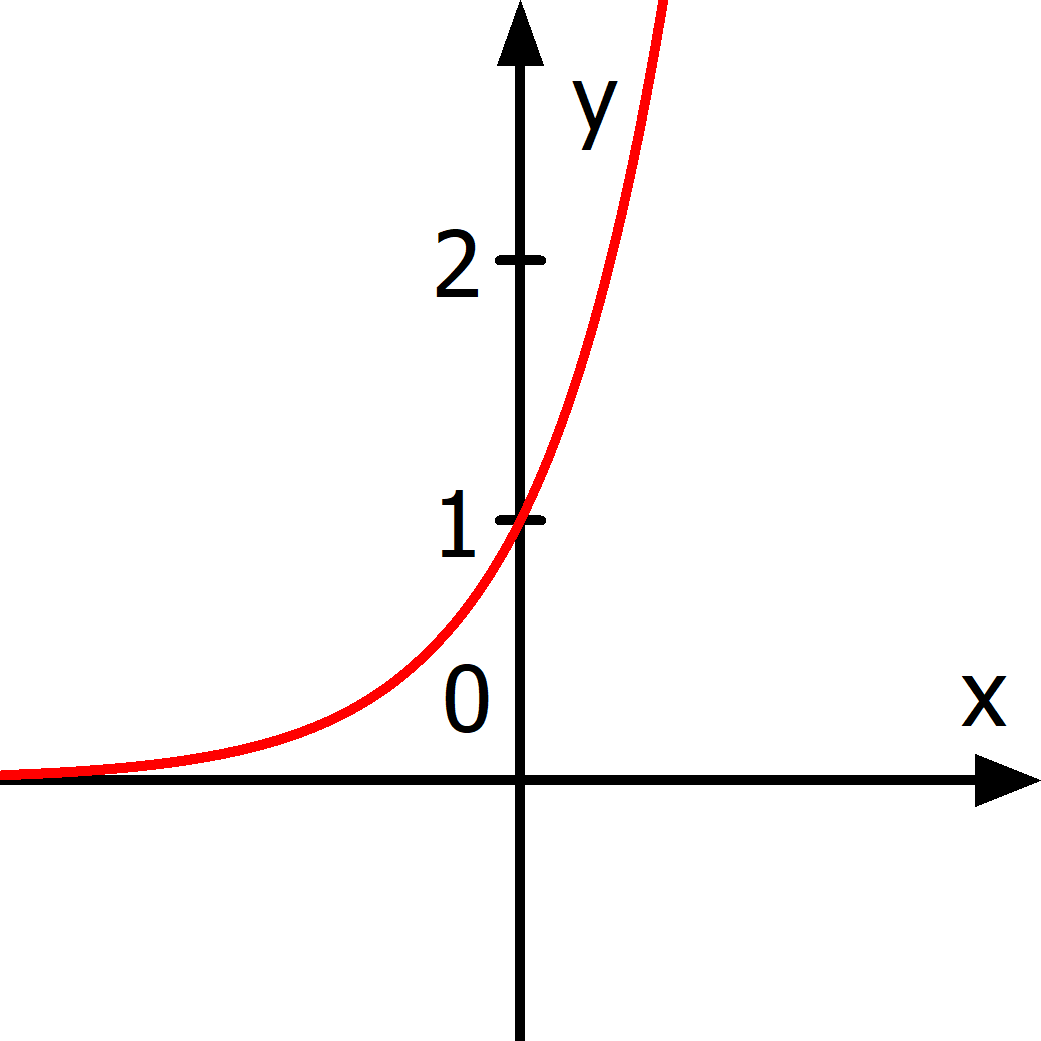
\includegraphics[width=.55\linewidth]{\eFkt/pics/A1a.png}
				\item \(f(x)=-3e^{\frac{1}{2}x}\)

				Asymptote \(y=0\)

				y-Achsenabschnitt: \(f(0)=-3\)

				Monoton fallend

				\(f(x)\xrightarrow{\hphantom{\ }x\to-\infty\hphantom{\ }}0\)

				\(f(x)\xrightarrow{\hphantom{\ }x\to\infty\hphantom{\ }}-\infty\)

				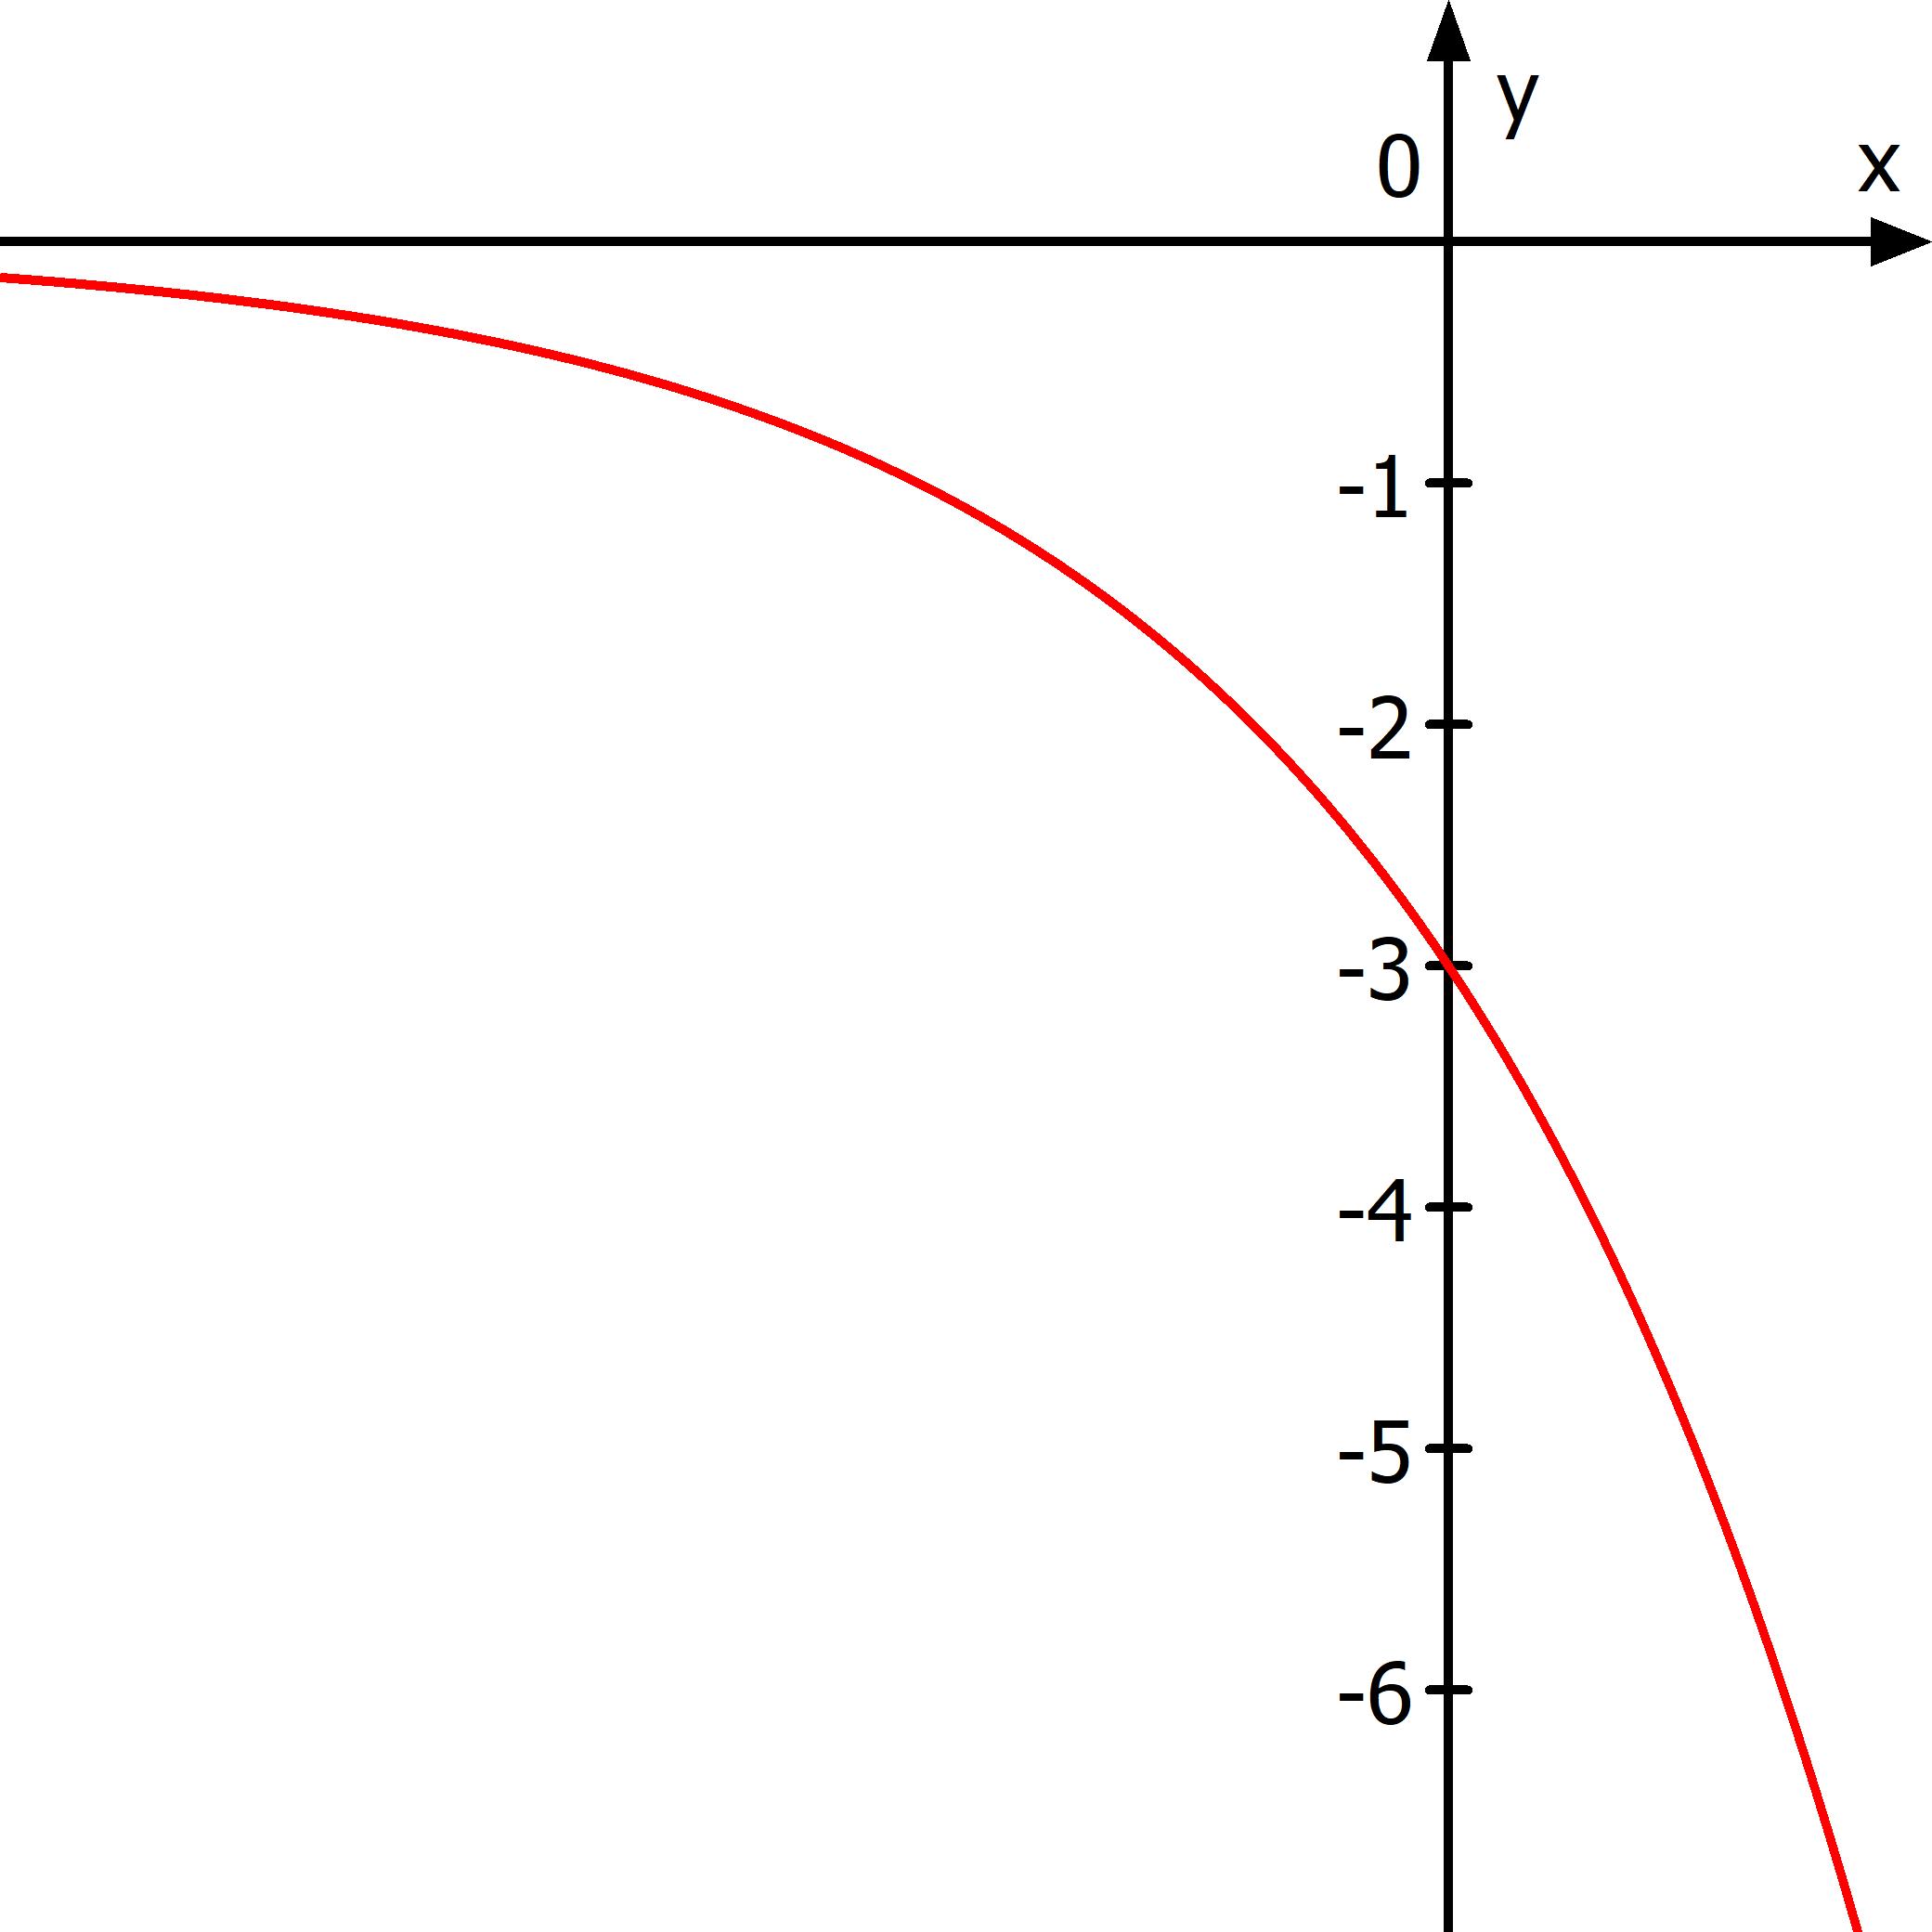
\includegraphics[width=.55\linewidth]{\eFkt/pics/A1b.png}
				\item \(f(x)=-4e^{-2x}\)

				Asymptote \(y=0\)

				y-Achsenabschnitt: \(f(0)=-4\)

				Monoton wachsend\\
				\(f(x)\xrightarrow{\hphantom{\ }x\to-\infty\hphantom{\ }}-\infty\)

				\(f(x)\xrightarrow{\hphantom{\ }x\to\infty\hphantom{\ }}0\)

				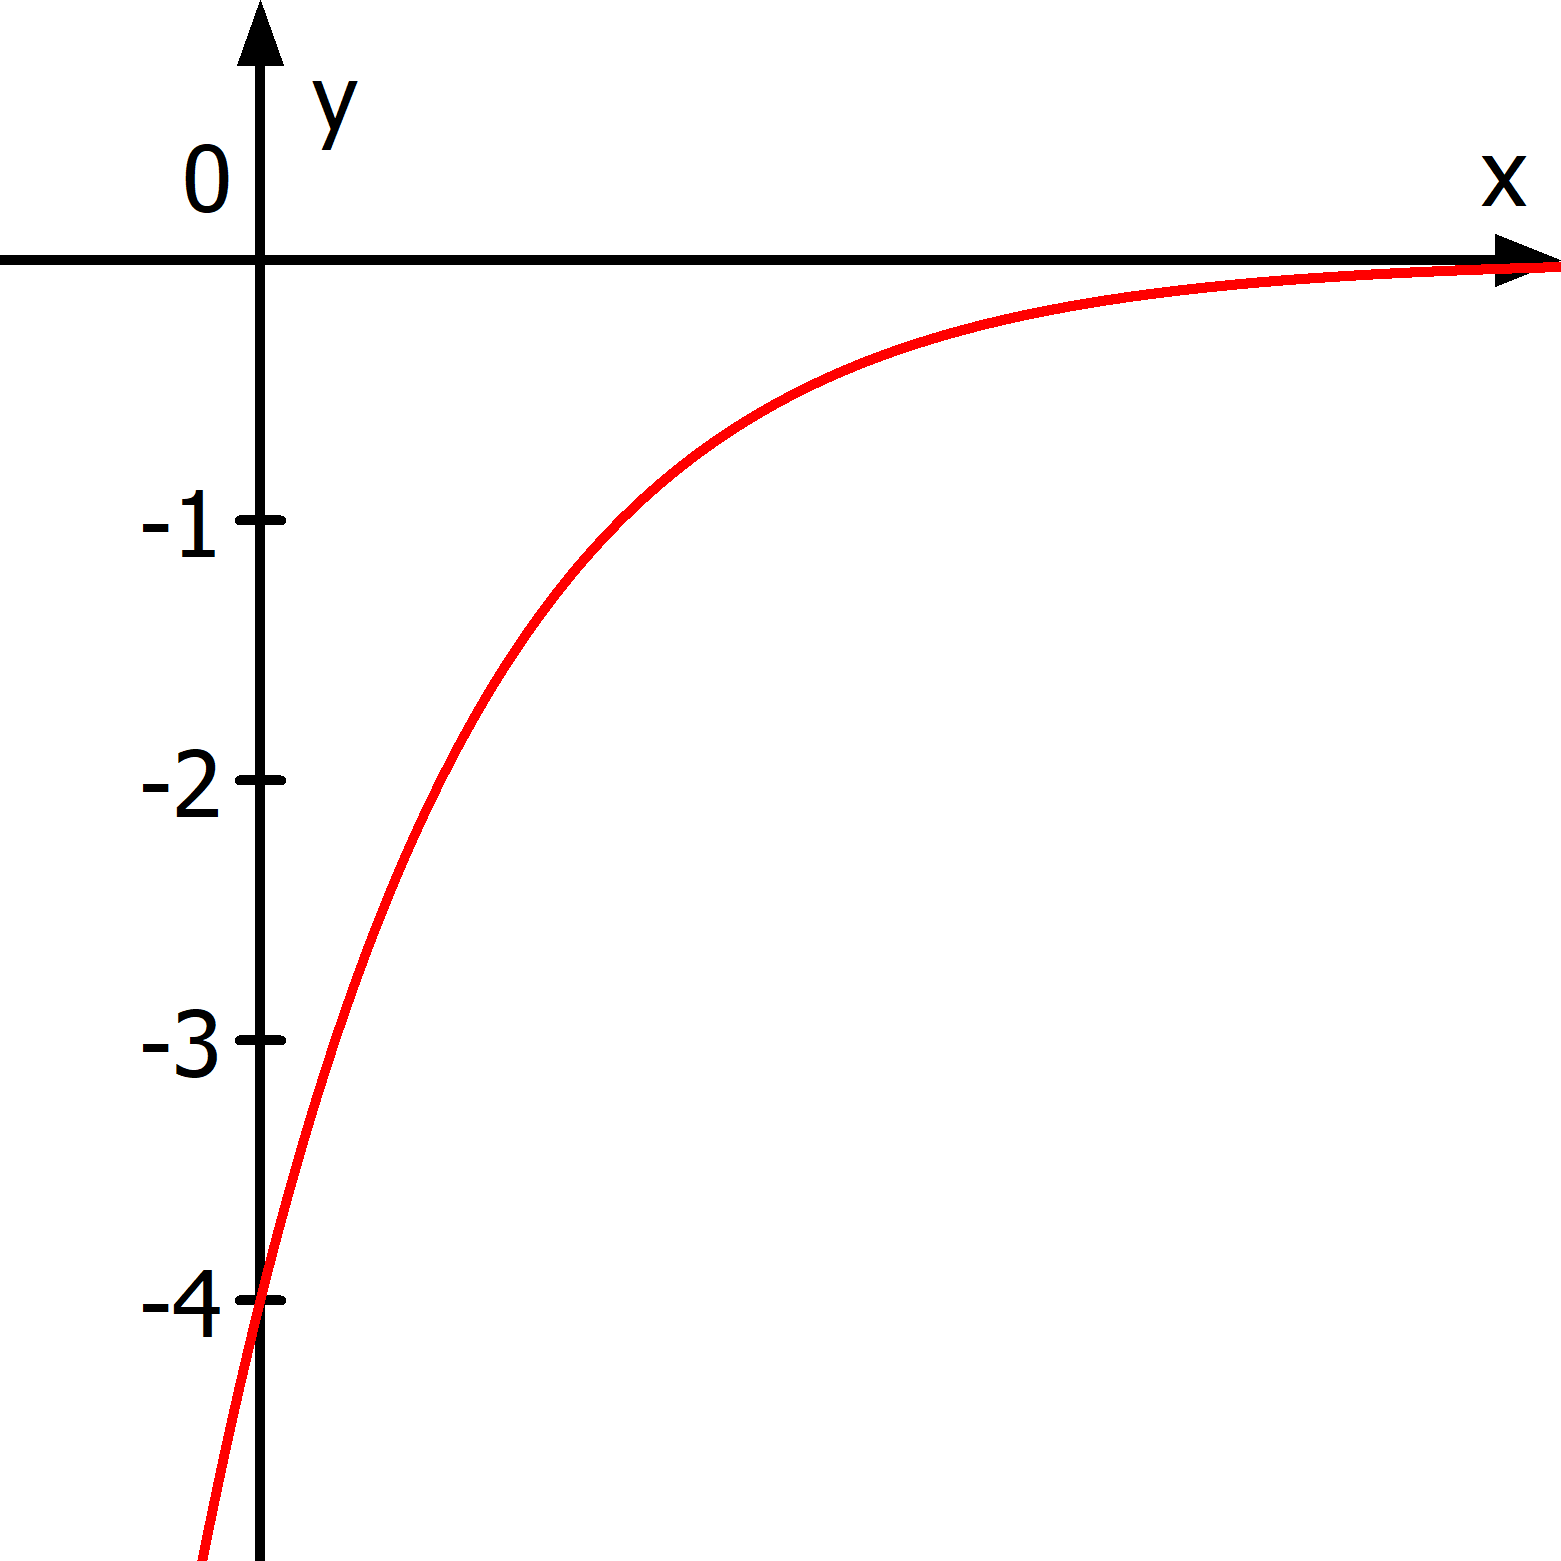
\includegraphics[width=.55\linewidth]{\eFkt/pics/A1c.png}
			\end{enumerate}
		\end{minipage}}%
		\adjustbox{valign=t}{\begin{minipage}{0.5\textwidth}
			\begin{enumerate}[label=\alph*)]
				\setcounter{enumi}{3}
				\item \(f(x)=2e^{-7x}\)

				Asymptote \(y=0\)

				y-Achsenabschnitt: \(f(0)=2\)

				Monoton fallend

				\(f(x)\xrightarrow{\hphantom{\ }x\to-\infty\hphantom{\ }}\infty\)

				\(f(x)\xrightarrow{\hphantom{\ }x\to\infty\hphantom{\ }}0\)

				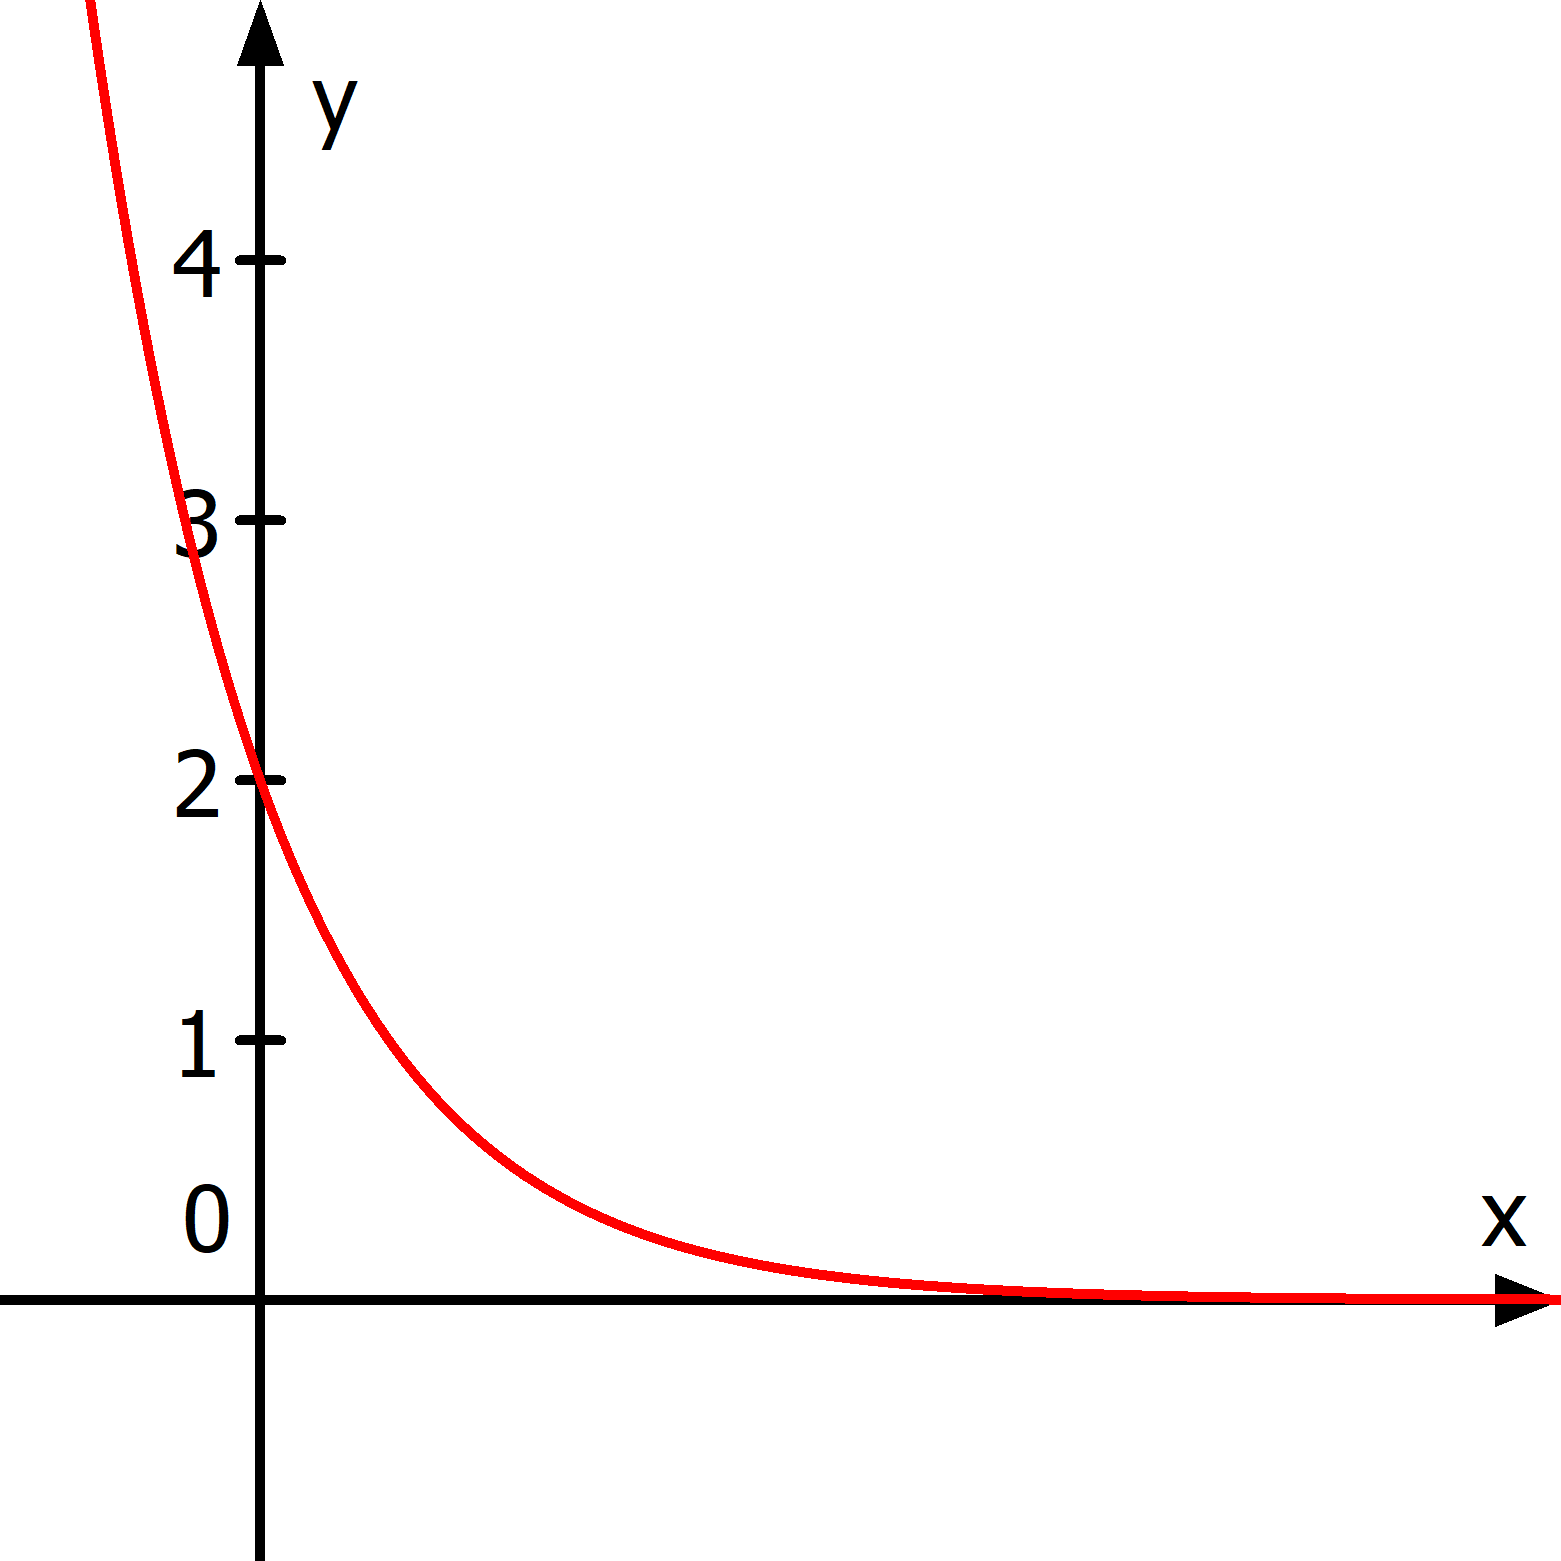
\includegraphics[width=.55\linewidth]{\eFkt/pics/A1d.png}
				\item \(f(x)=-\frac{5}{3}e^{x}\)

				Asymptote \(y=0\)

				y-Achsenabschnitt: \(f(0)=-\frac{5}{3}\)

				Monoton fallend

				\(f(x)\xrightarrow{\hphantom{\ }x\to-\infty\hphantom{\ }}0\)

				\(f(x)\xrightarrow{\hphantom{\ }x\to\infty\hphantom{\ }}-\infty\)

				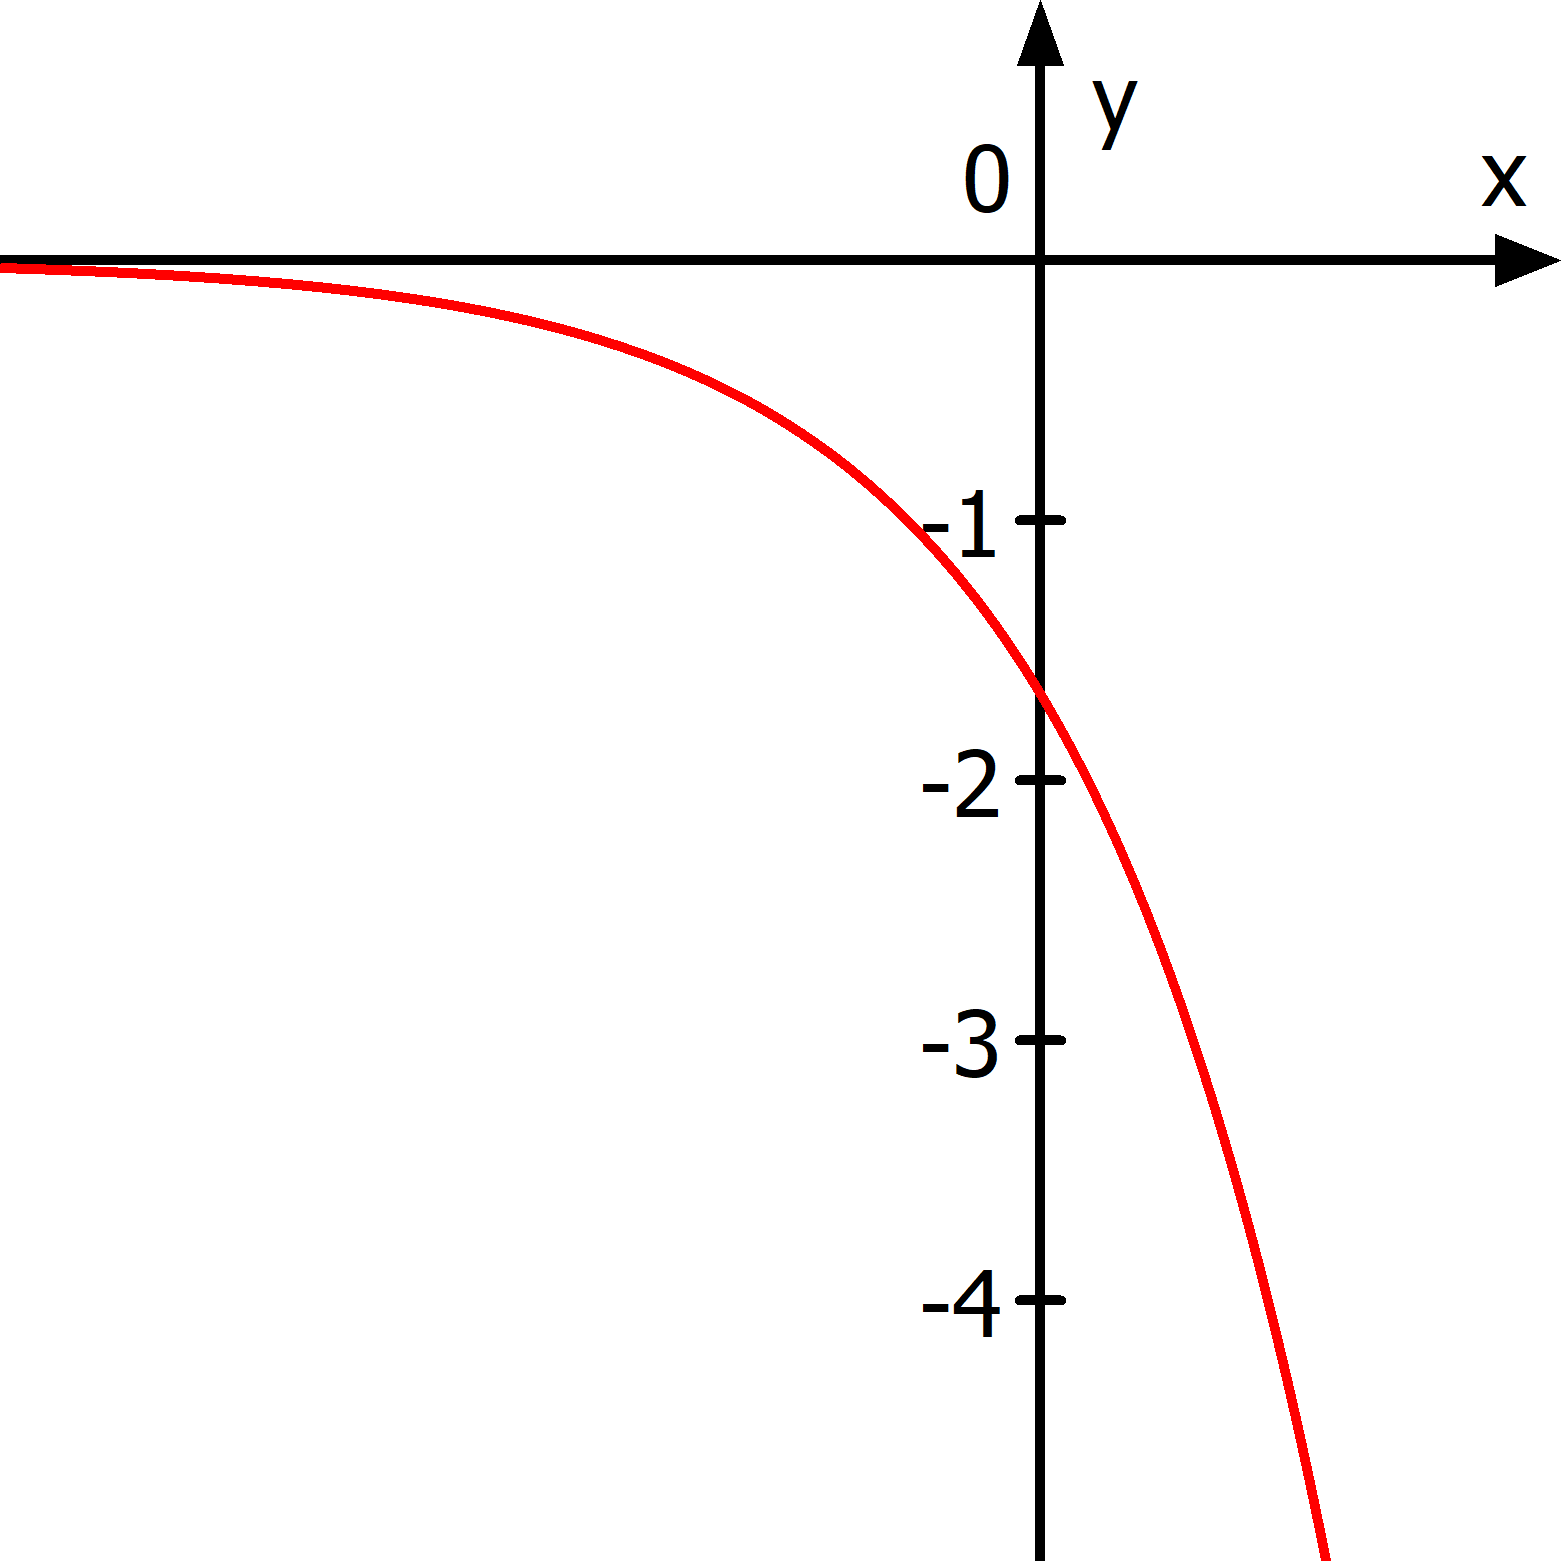
\includegraphics[width=.55\linewidth]{\eFkt/pics/A1e.png}
				\item \(f(x)=8e^{-3x}\)

				Asymptote \(y=0\)

				y-Achsenabschnitt: \(f(0)=8\)

				Monoton fallend

				\(f(x)\xrightarrow{\hphantom{\ }x\to-\infty\hphantom{\ }}\infty\)

				\(f(x)\xrightarrow{\hphantom{\ }x\to\infty\hphantom{\ }}0\)

				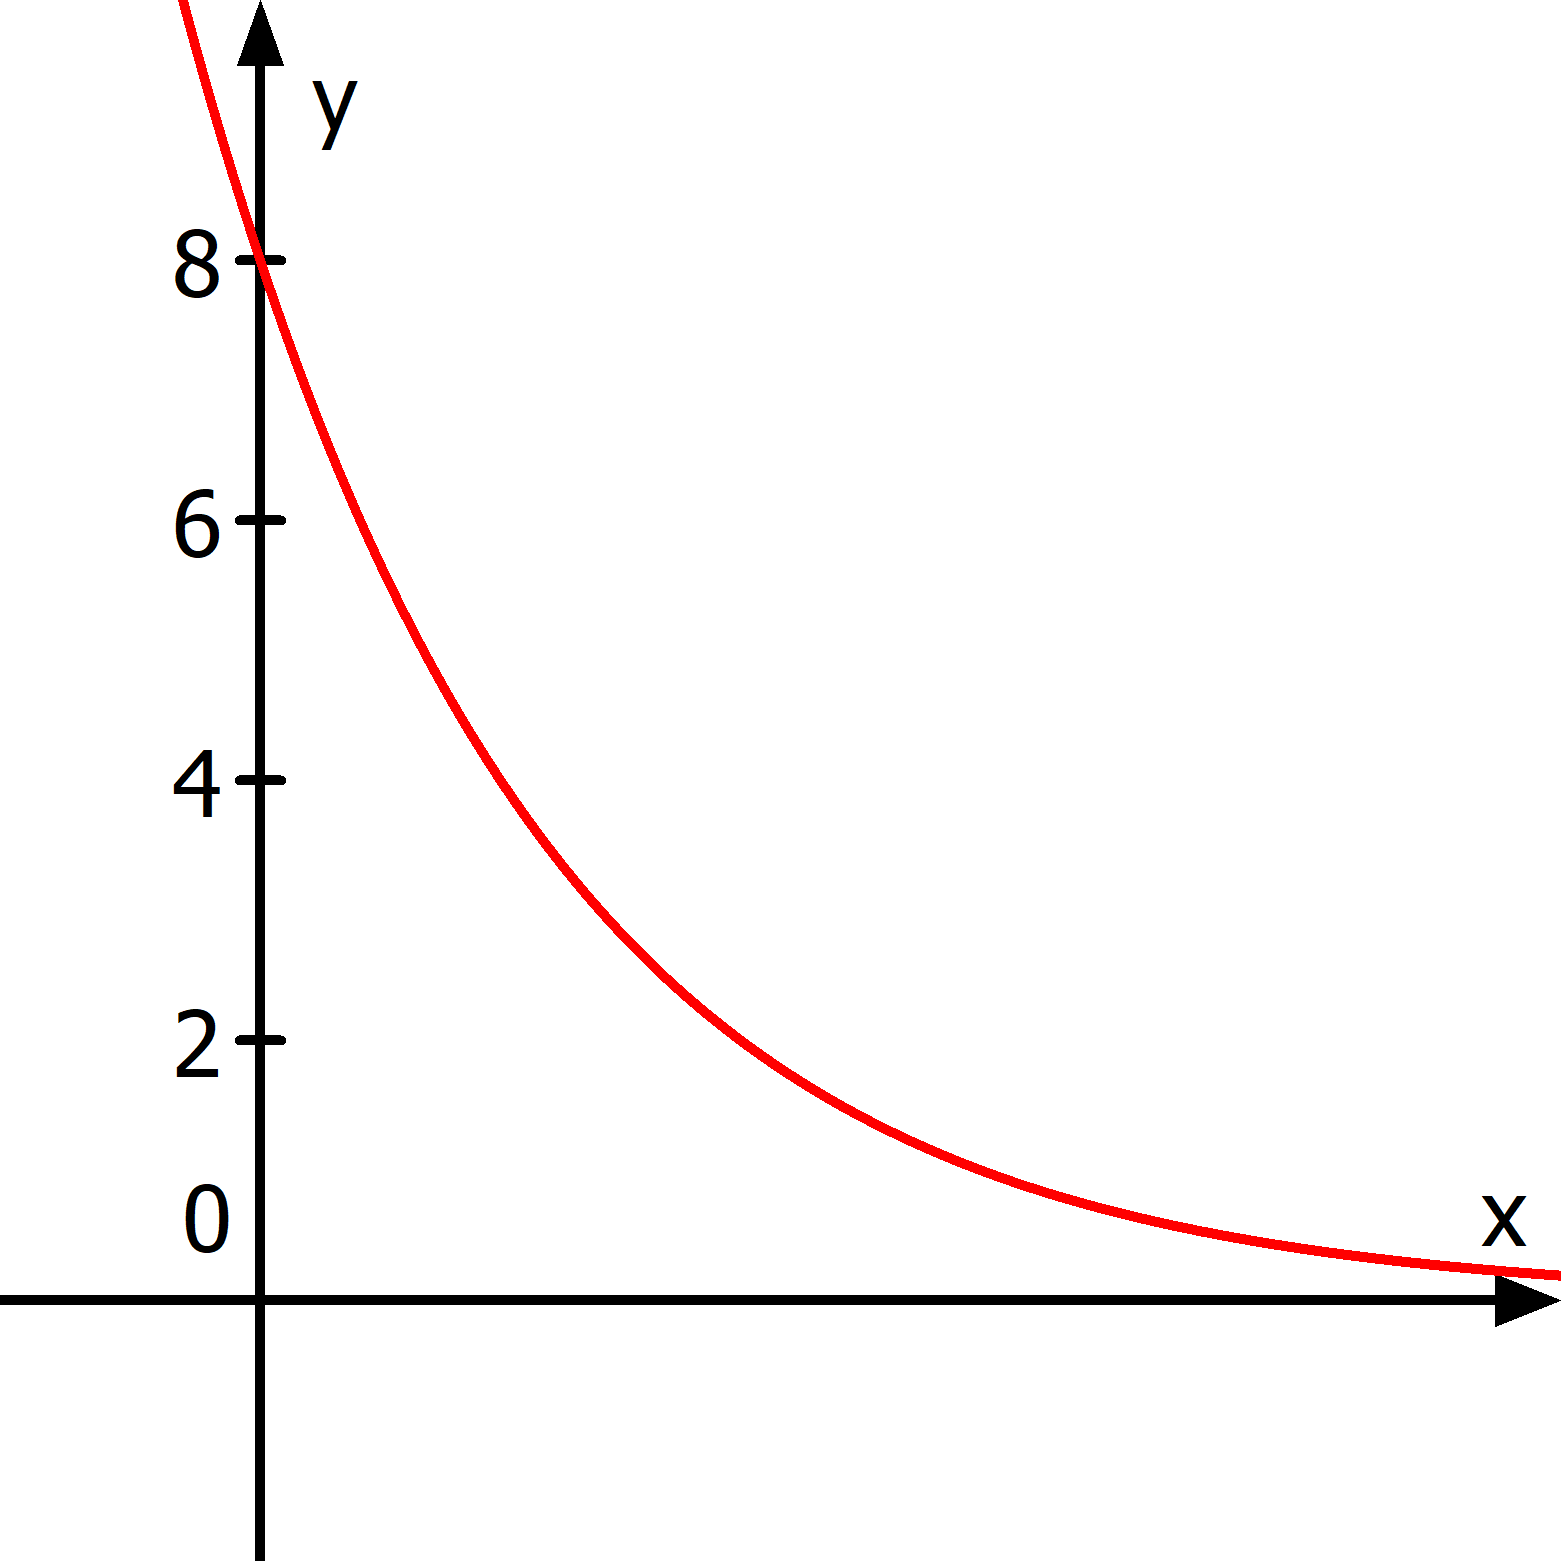
\includegraphics[width=.55\linewidth]{\eFkt/pics/A1f.png}
			\end{enumerate}
		\end{minipage}}%
	\end{minipage}%

	%%%%% g bis l
	\begin{minipage}{\textwidth}
		\adjustbox{valign=t}{\begin{minipage}{0.5\textwidth}
			\begin{enumerate}[label=\alph*)]
				\setcounter{enumi}{6}
				\item \(f(x)=-3e^{-\frac{9}{8}x}\)

				Asymptote \(y=0\)

				y-Achsenabschnitt: \(f(0)=-3\)

				Monoton wachsend

				\(f(x)\xrightarrow{\hphantom{\ }x\to-\infty\hphantom{\ }}-\infty\)

				\(f(x)\xrightarrow{\hphantom{\ }x\to\infty\hphantom{\ }}0\)

				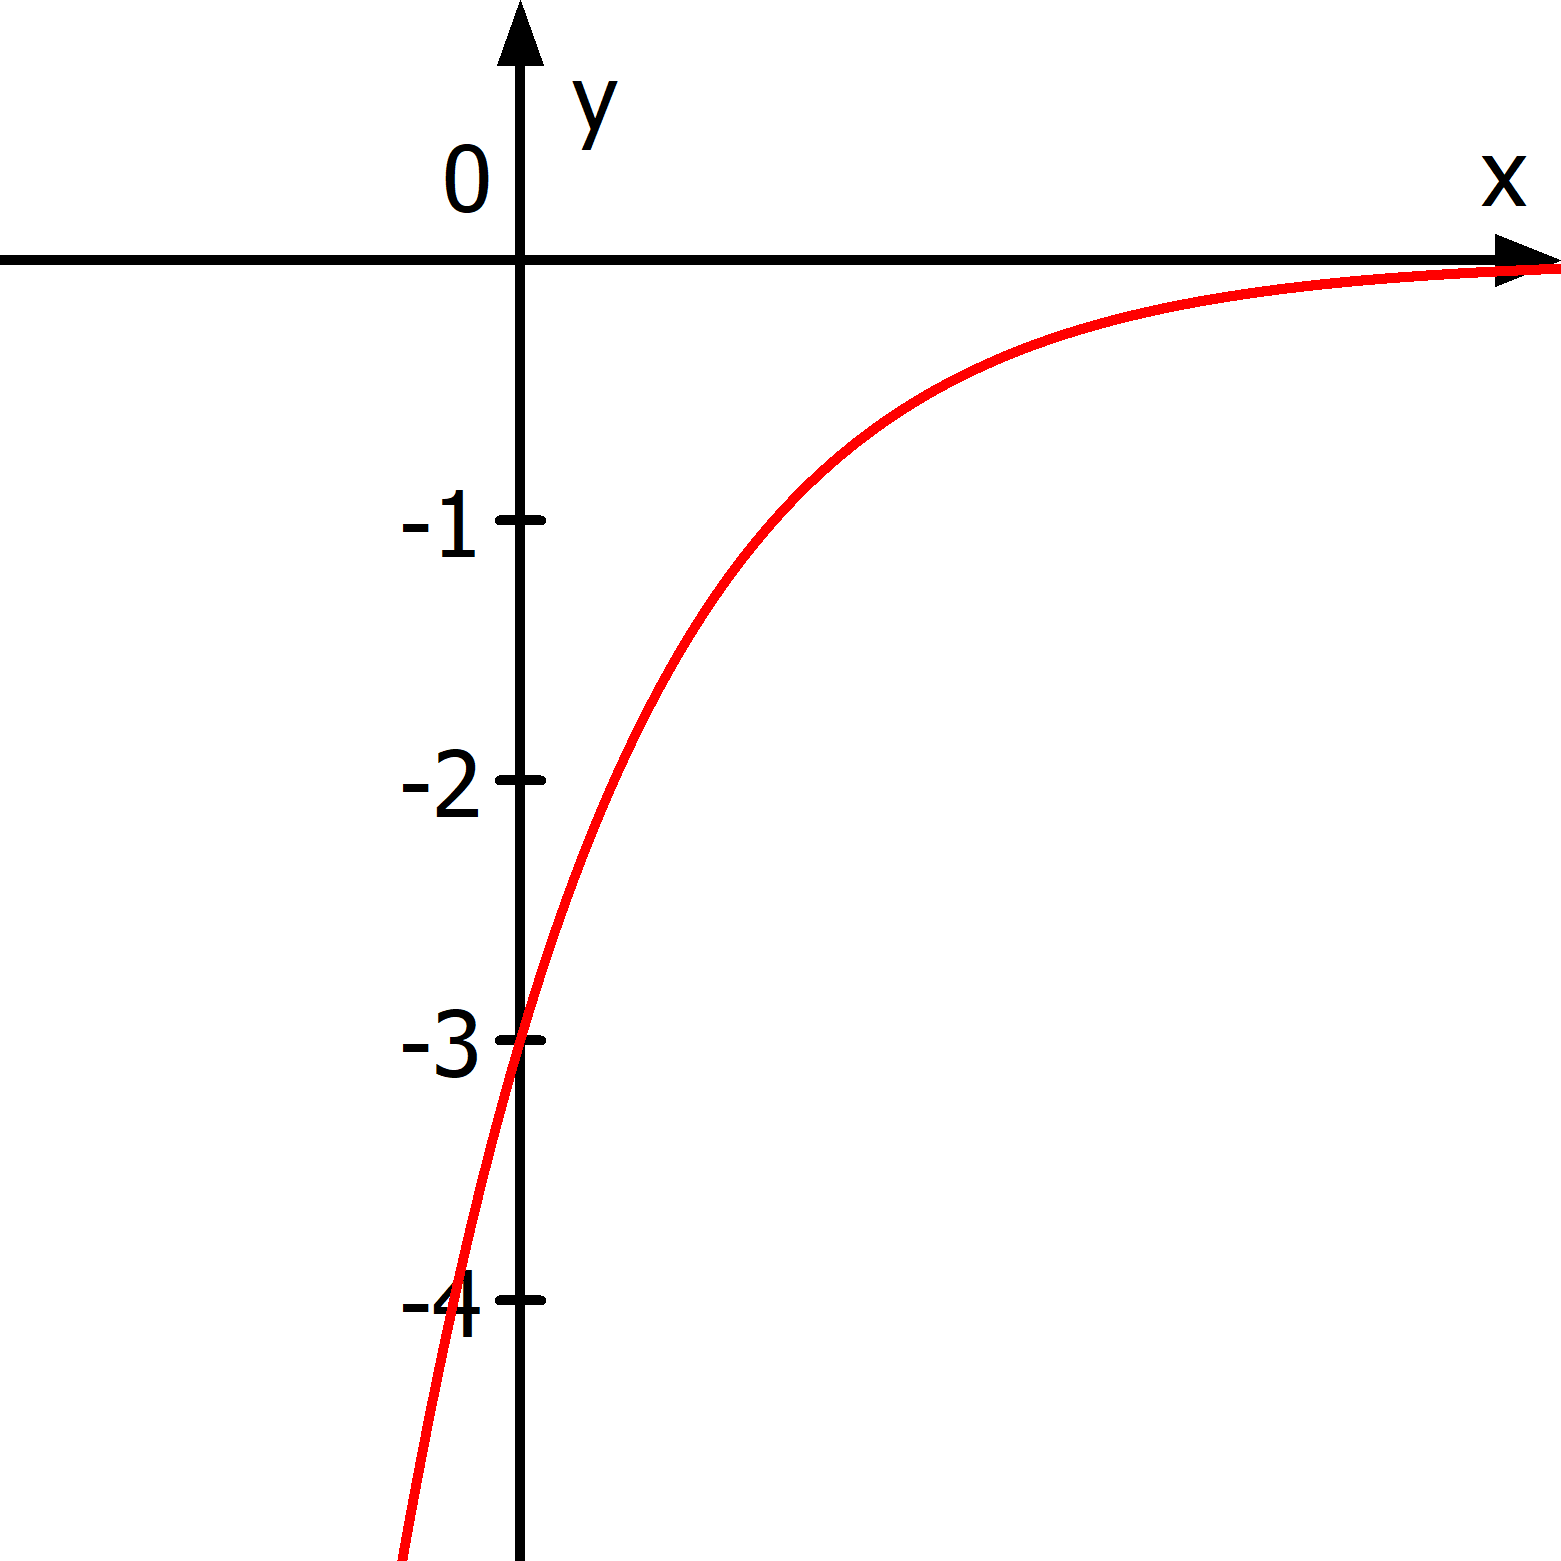
\includegraphics[width=.6\linewidth]{\eFkt/pics/A1g.png}
				\item \(f(x)=\frac{3}{5}e^{0,2x}\)

				Asymptote \(y=0\)

				y-Achsenabschnitt: \(f(0)=\frac{3}{5}\)

				Monoton wachsend

				\(f(x)\xrightarrow{\hphantom{\ }x\to-\infty\hphantom{\ }}0\)

				\(f(x)\xrightarrow{\hphantom{\ }x\to\infty\hphantom{\ }}\infty\)

				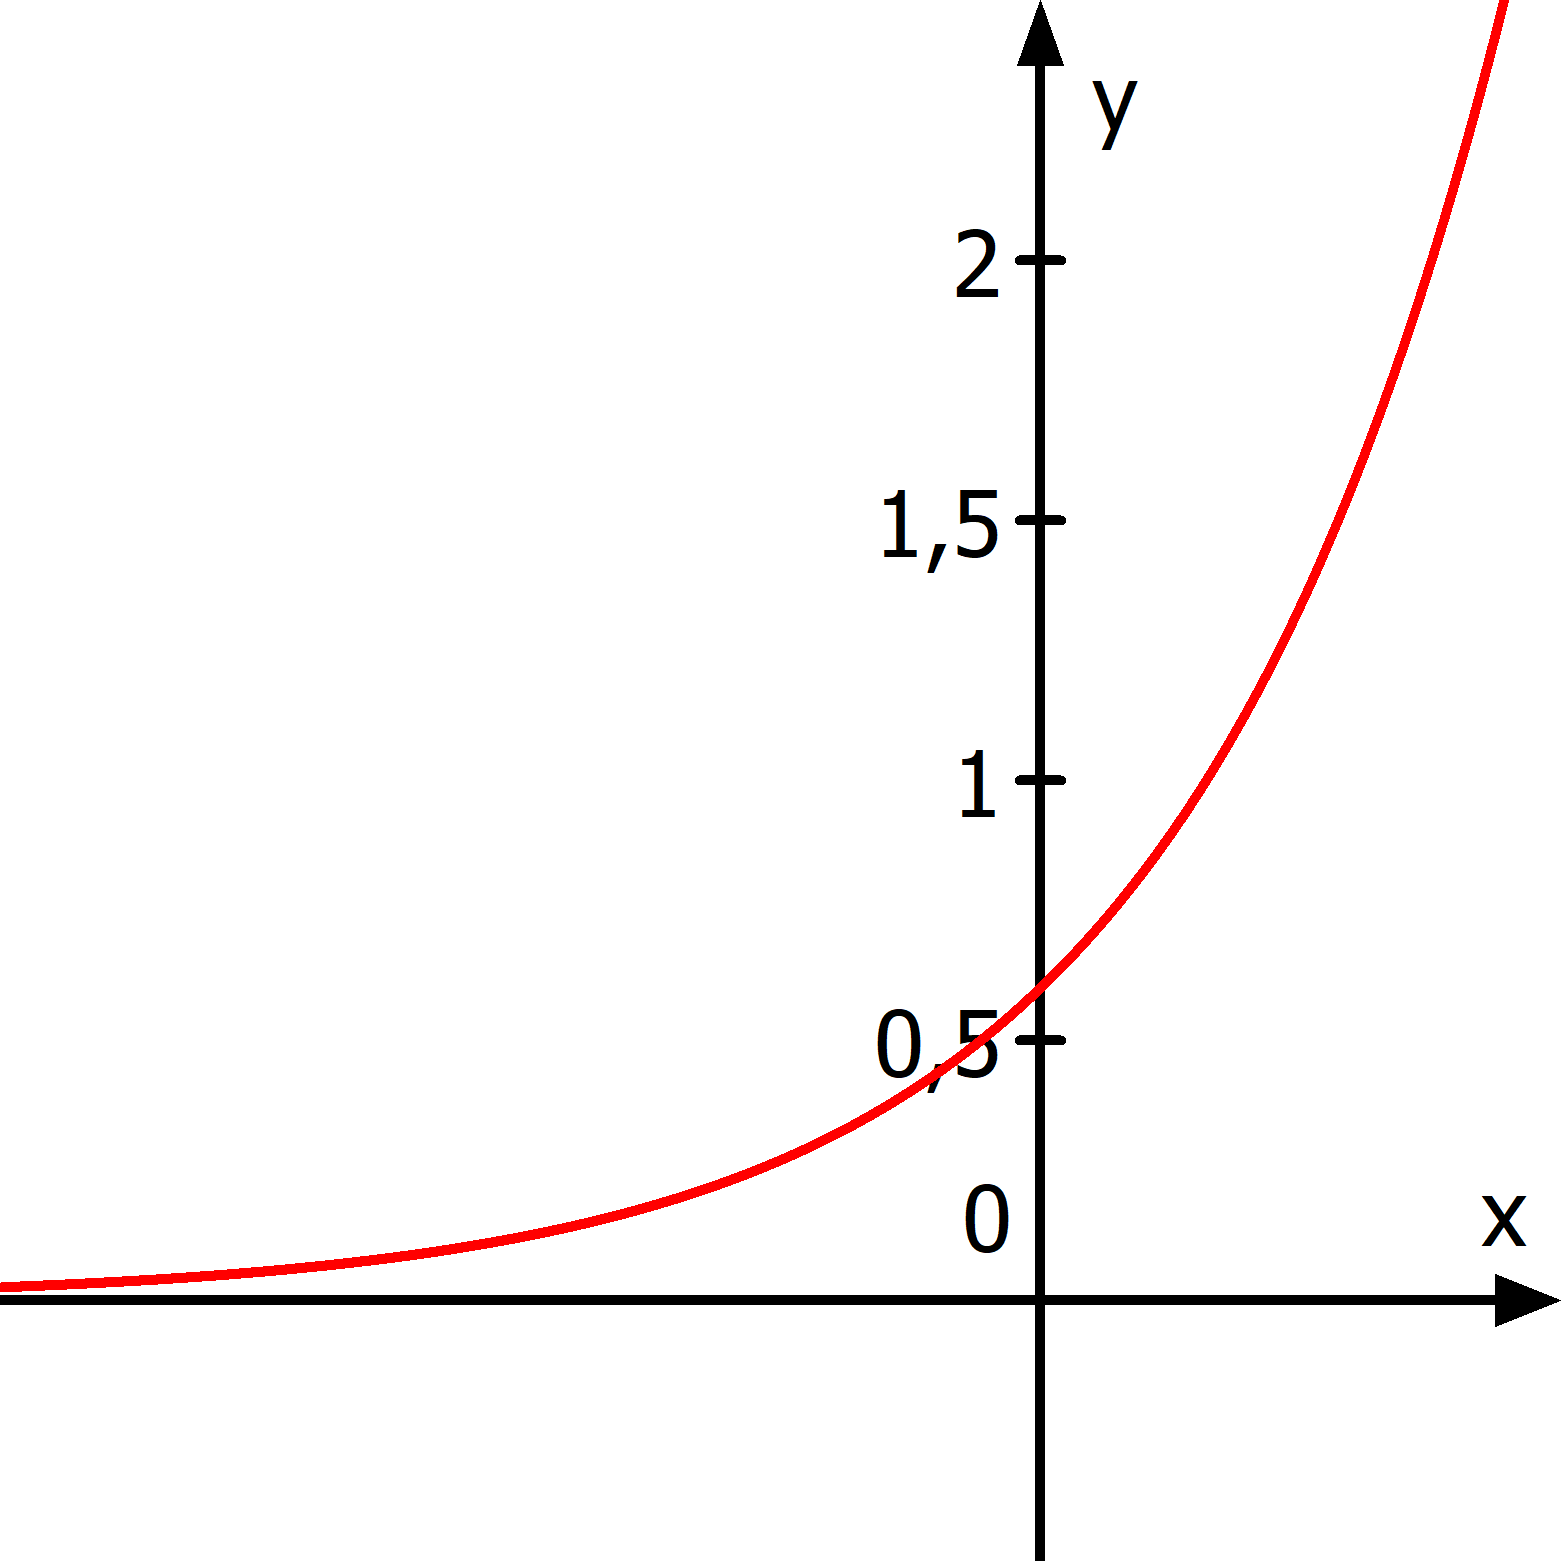
\includegraphics[width=.6\linewidth]{\eFkt/pics/A1h.png}
				\item \(f(x)=-0,5e^{-3,5x}\)

				Asymptote \(y=0\)

				y-Achsenabschnitt: \(f(0)=-0,5\)

				Monoton wachsend

				\(f(x)\xrightarrow{\hphantom{\ }x\to-\infty\hphantom{\ }}-\infty\)

				\(f(x)\xrightarrow{\hphantom{\ }x\to\infty\hphantom{\ }}0\)

				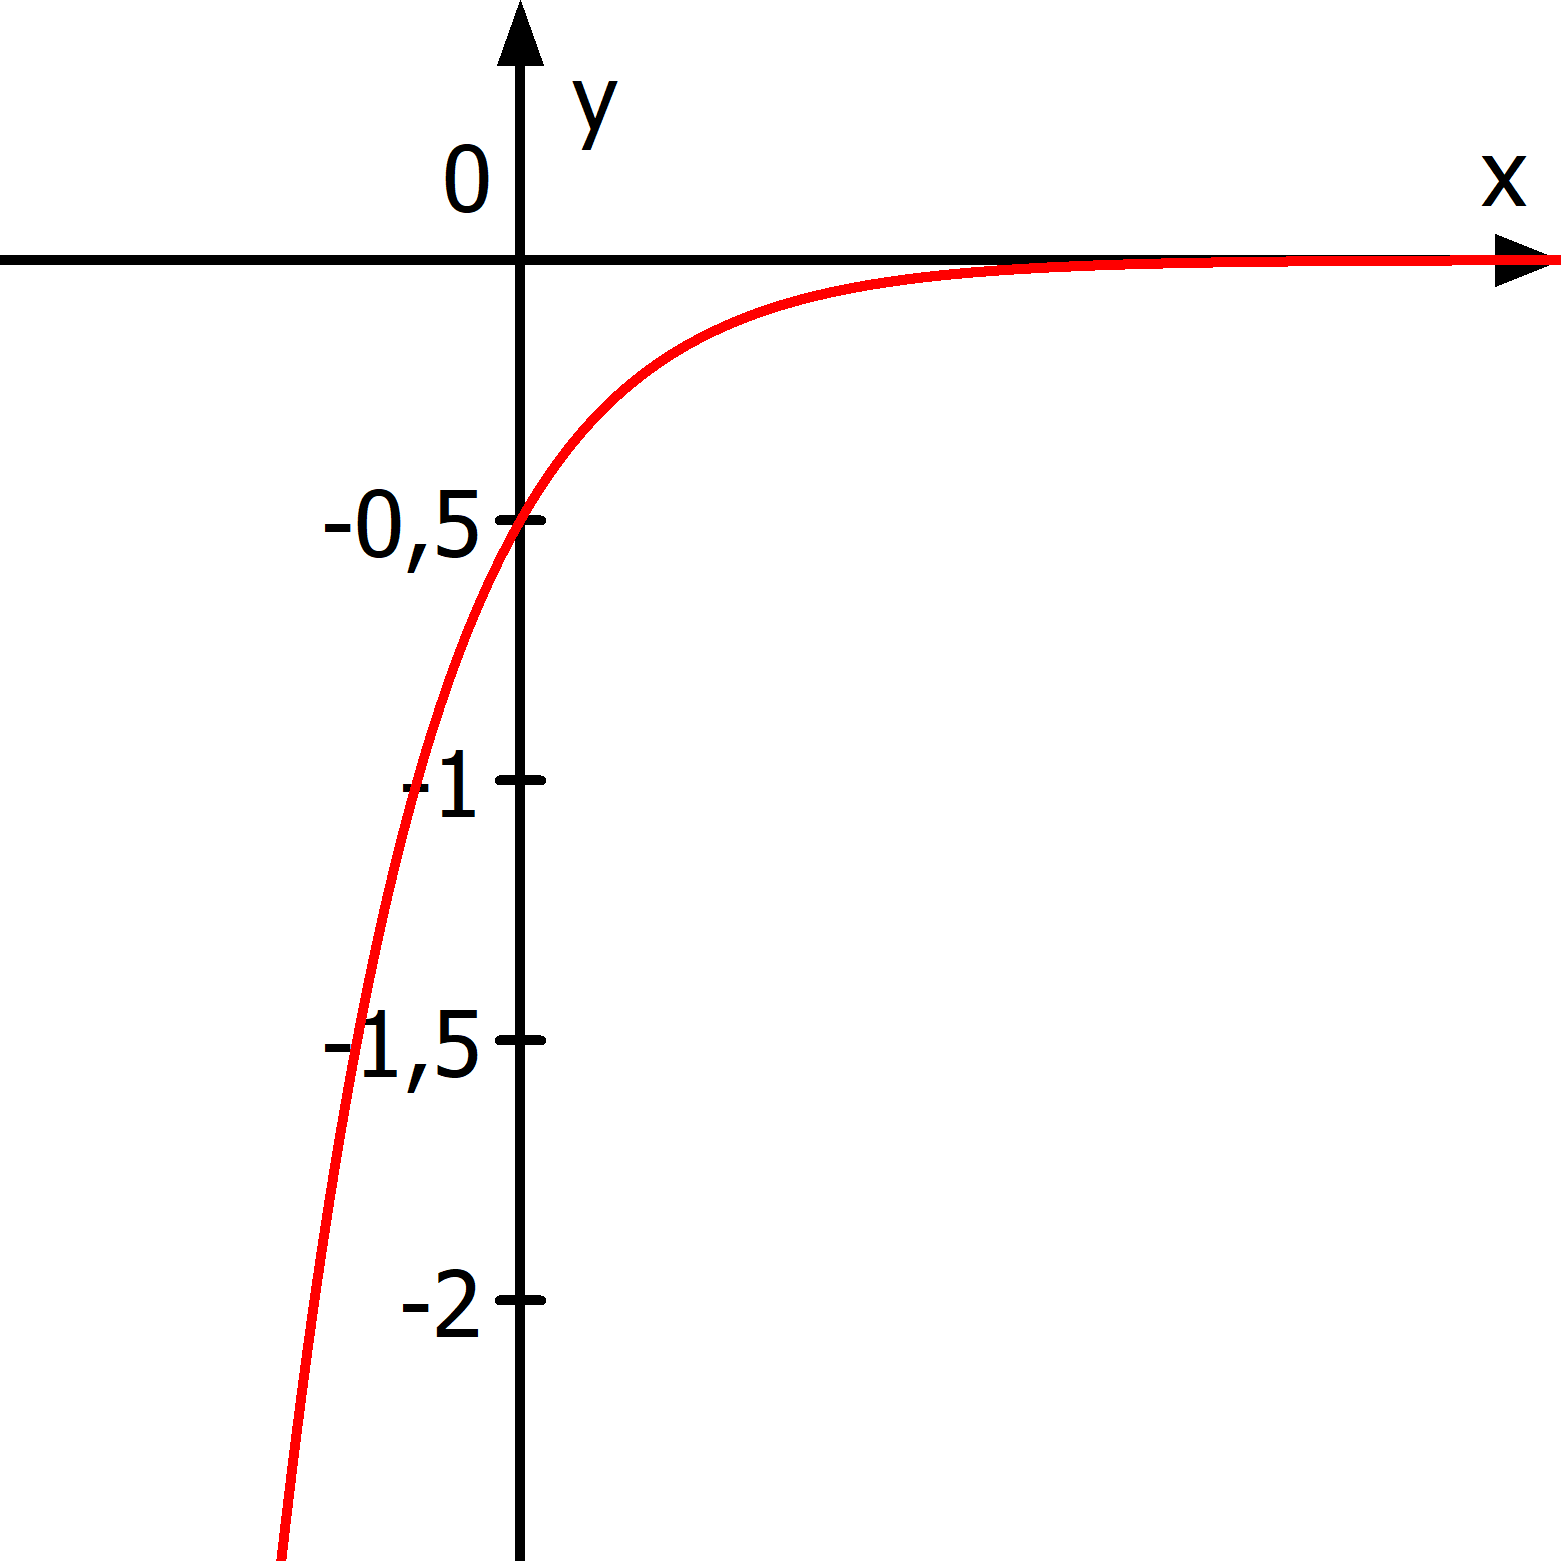
\includegraphics[width=.6\linewidth]{\eFkt/pics/A1i.png}
			\end{enumerate}
		\end{minipage}}%
		\adjustbox{valign=t}{\begin{minipage}{0.5\textwidth}
			\begin{enumerate}[label=\alph*)]
				\setcounter{enumi}{9}
				\item \(f(x)=-8e^{\frac{1}{10}x}\)

				Asymptote \(y=0\)

				y-Achsenabschnitt: \(f(0)=-8\)

				Monoton fallend

				\(f(x)\xrightarrow{\hphantom{\ }x\to-\infty\hphantom{\ }}0\)

				\(f(x)\xrightarrow{\hphantom{\ }x\to\infty\hphantom{\ }}-\infty\)

				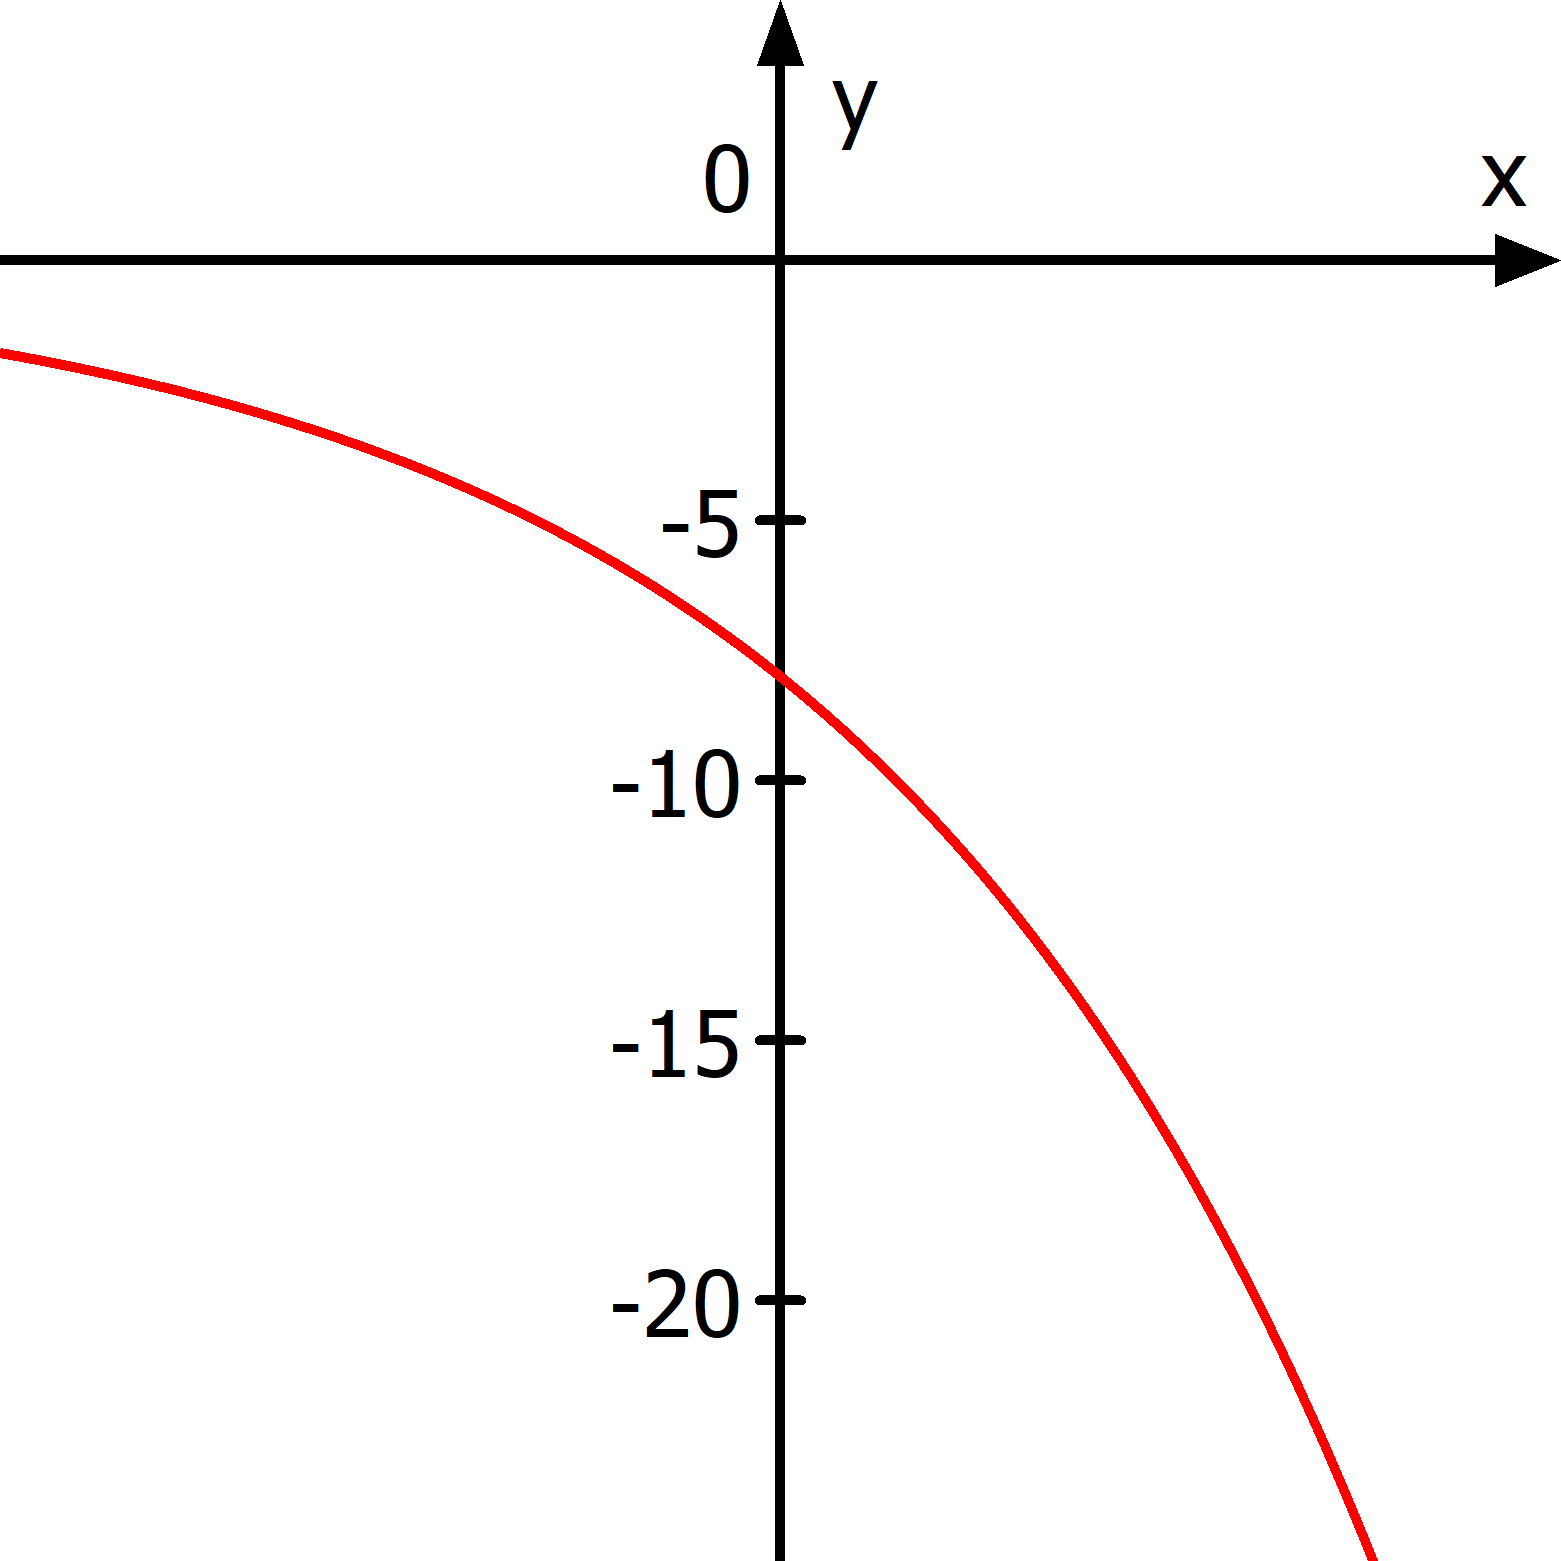
\includegraphics[width=.6\linewidth]{\eFkt/pics/A1j.png}
				\item \(f(x)=2e^{-2x}\)

				Asymptote \(y=0\)

				y-Achsenabschnitt: \(f(0)=2\)

				Monoton fallend

				\(f(x)\xrightarrow{\hphantom{\ }x\to-\infty\hphantom{\ }}\infty\)

				\(f(x)\xrightarrow{\hphantom{\ }x\to\infty\hphantom{\ }}0\)

				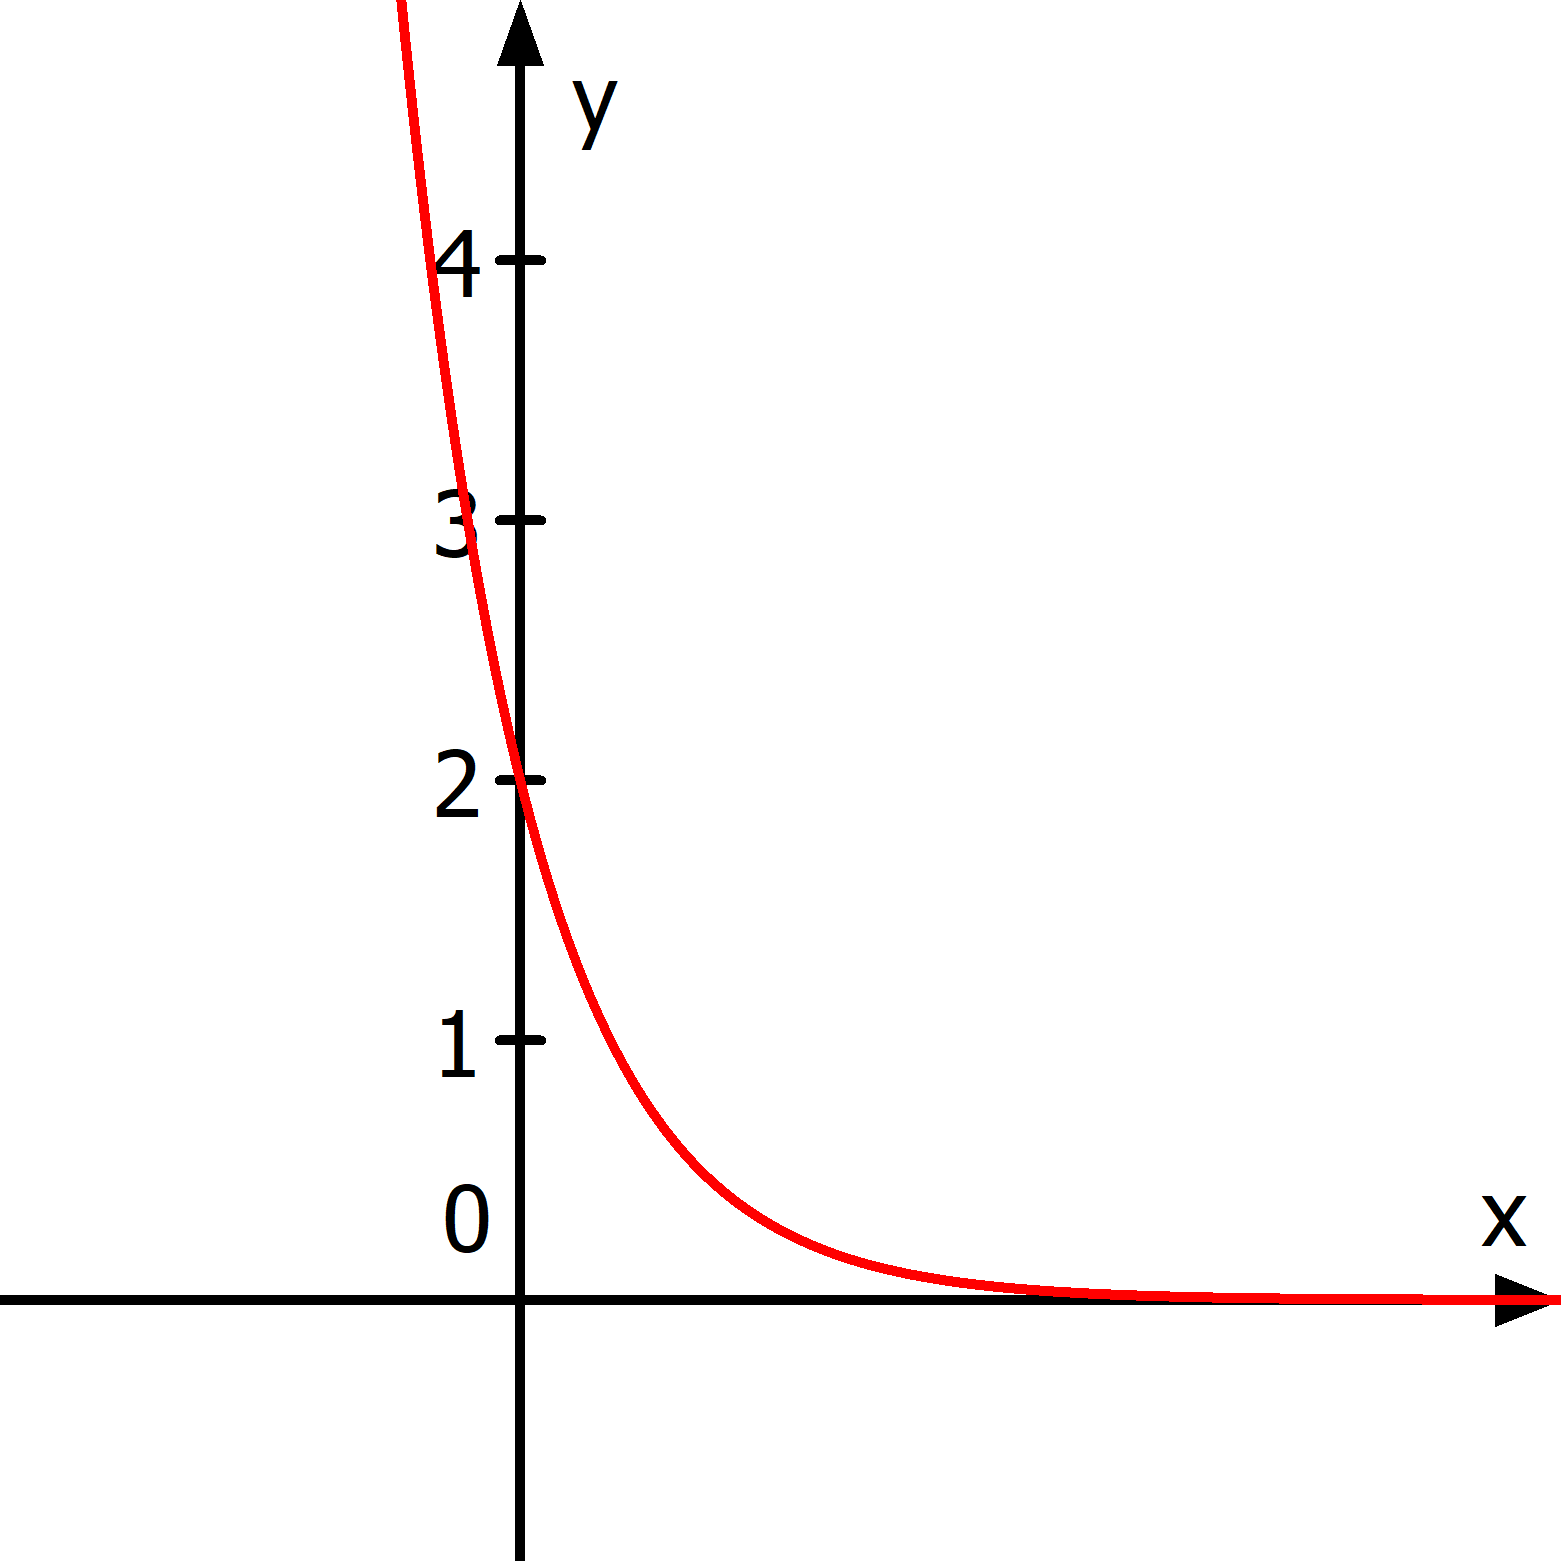
\includegraphics[width=.6\linewidth]{\eFkt/pics/A1k.png}
				\item \(f(x)=-4e^{-7x}\)

				Asymptote \(y=0\)

				y-Achsenabschnitt: \(f(0)=-4\)

				Monoton wachsend

				\(f(x)\xrightarrow{\hphantom{\ }x\to-\infty\hphantom{\ }}-\infty\)

				\(f(x)\xrightarrow{\hphantom{\ }x\to\infty\hphantom{\ }}0\)

				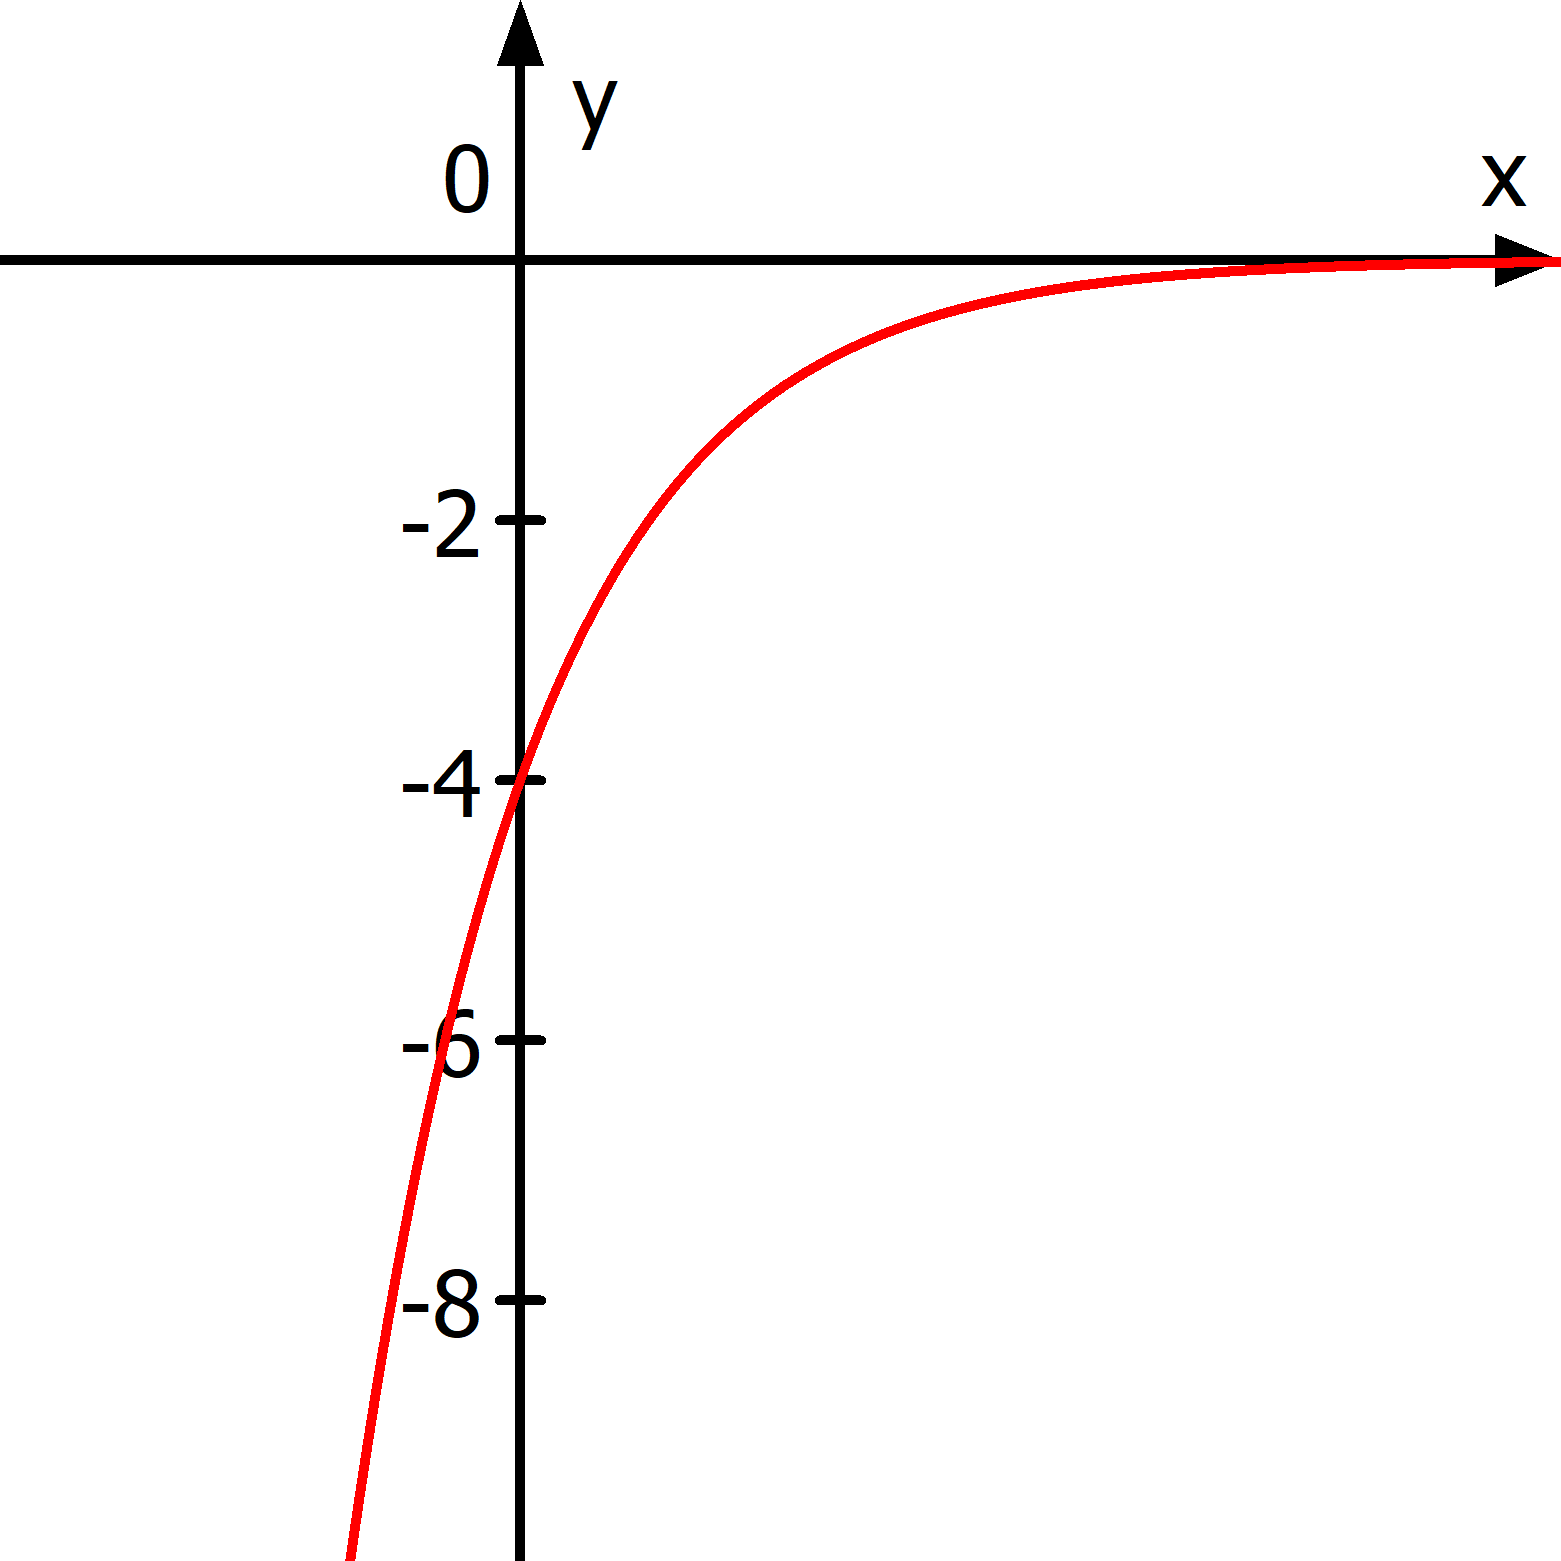
\includegraphics[width=.6\linewidth]{\eFkt/pics/A1l.png}
			\end{enumerate}
		\end{minipage}}%
	\end{minipage}

	%%%%% m bis r
	\begin{minipage}{\textwidth}
		\adjustbox{valign=t}{\begin{minipage}{0.5\textwidth}
			\begin{enumerate}[label=\alph*)]
				\setcounter{enumi}{12}
				\item \(f(x)=-\frac{5}{7}e^{x}\)

				Asymptote \(y=0\)

				y-Achsenabschnitt: \(f(0)=-\frac{5}{7}\)

				Monoton fallend

				\(f(x)\xrightarrow{\hphantom{\ }x\to-\infty\hphantom{\ }}0\)

				\(f(x)\xrightarrow{\hphantom{\ }x\to\infty\hphantom{\ }}-\infty\)

				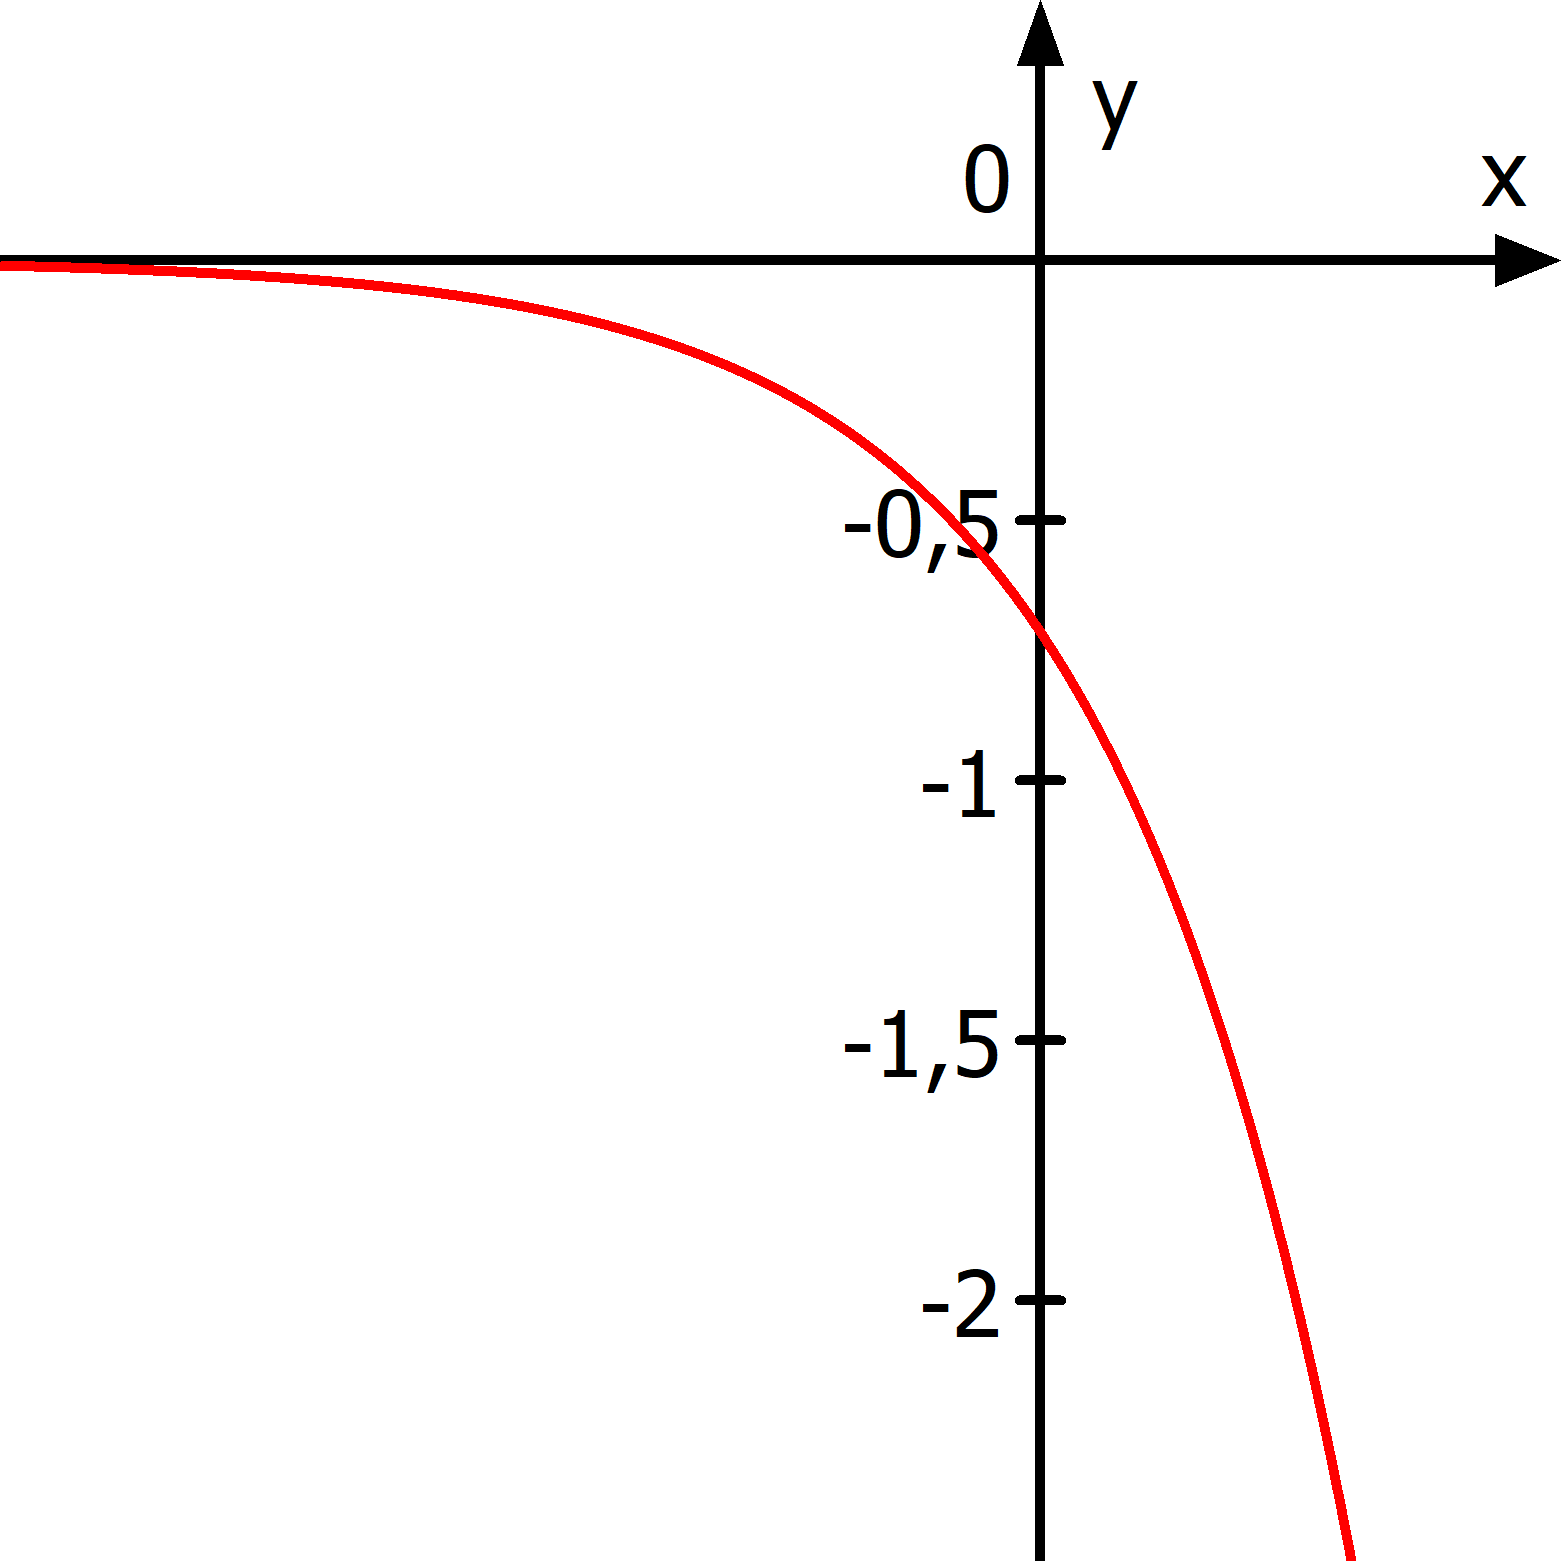
\includegraphics[width=.6\linewidth]{\eFkt/pics/A1m.png}
				\item \(f(x)=6e^{-4x}\)

				Asymptote \(y=0\)

				y-Achsenabschnitt: \(f(0)=6\)

				Monoton fallend

				\(f(x)\xrightarrow{\hphantom{\ }x\to-\infty\hphantom{\ }}\infty\)

				\(f(x)\xrightarrow{\hphantom{\ }x\to\infty\hphantom{\ }}0\)

				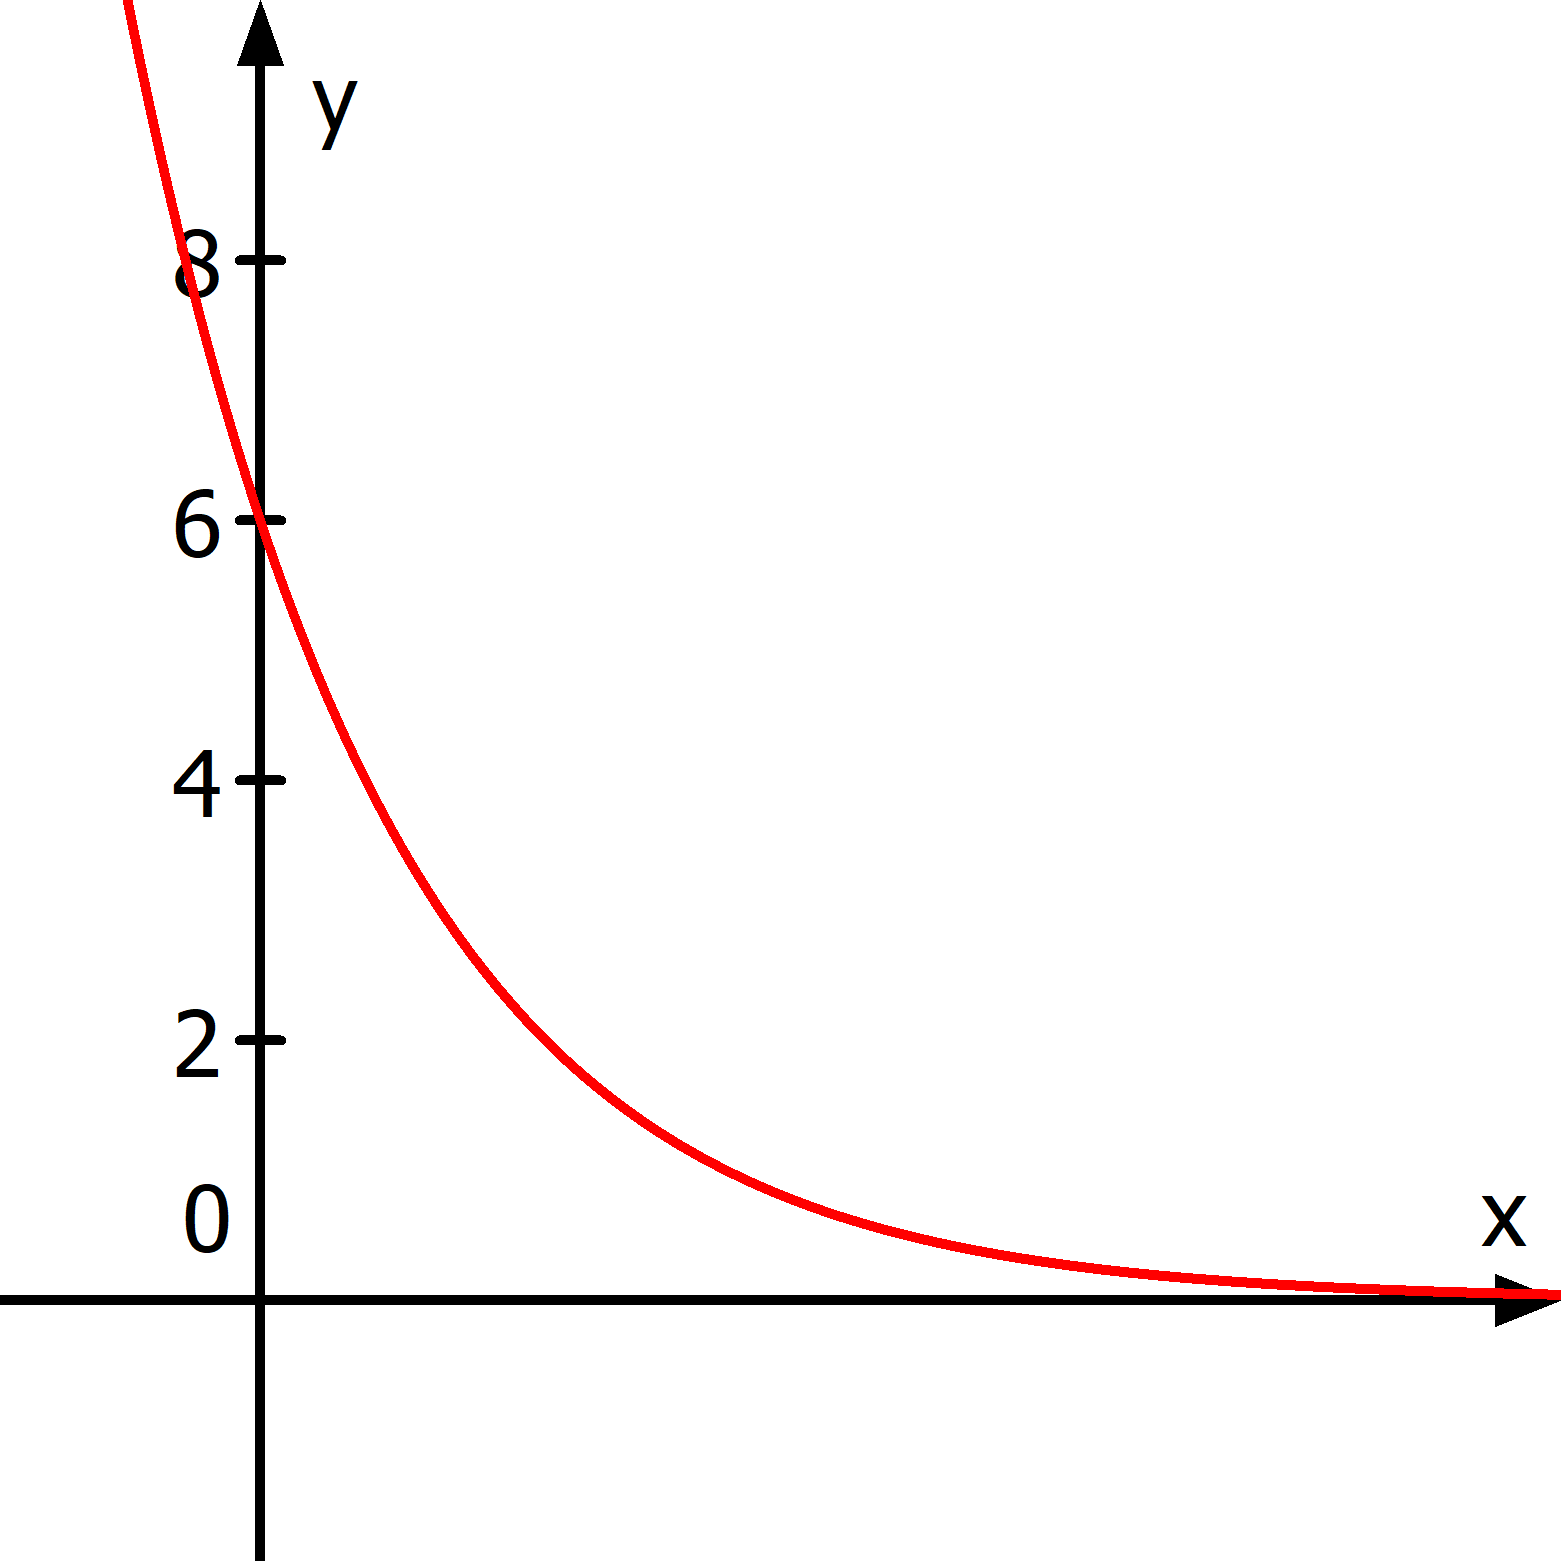
\includegraphics[width=.6\linewidth]{\eFkt/pics/A1n.png}
				\item \(f(x)=-2e^{-8x}\)

				Asymptote \(y=0\)

				y-Achsenabschnitt: \(f(0)=-2\)

				Monoton wachsend

				\(f(x)\xrightarrow{\hphantom{\ }x\to-\infty\hphantom{\ }}-\infty\)

				\(f(x)\xrightarrow{\hphantom{\ }x\to\infty\hphantom{\ }}0\)

				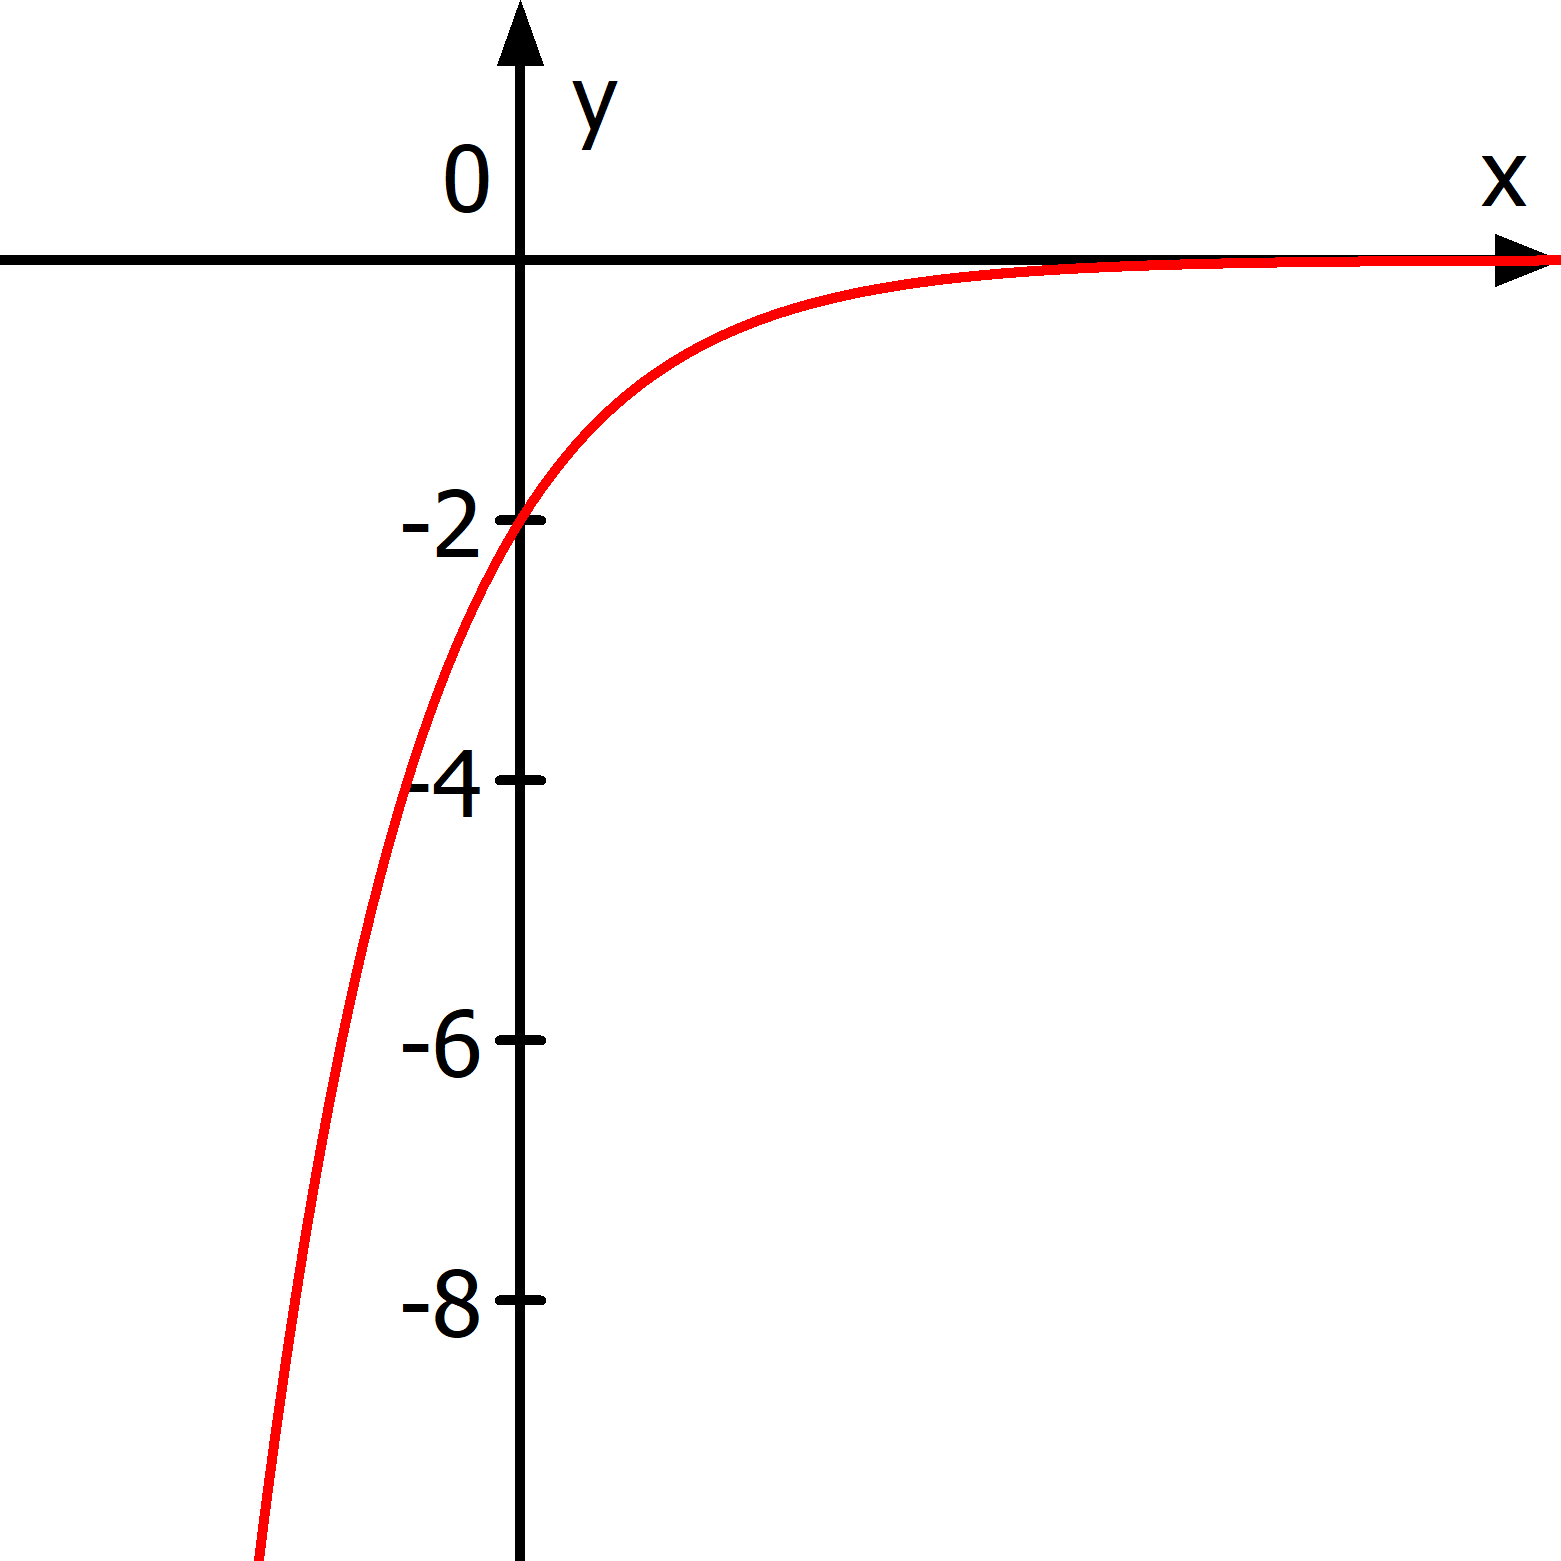
\includegraphics[width=.6\linewidth]{\eFkt/pics/A1o.png}
			\end{enumerate}
		\end{minipage}}%
		\adjustbox{valign=t}{\begin{minipage}{0.5\textwidth}
			\begin{enumerate}[label=\alph*)]
				\setcounter{enumi}{15}
				\item \(f(x)=5,3e^{0,2x}\)

				Asymptote \(y=0\)

				y-Achsenabschnitt: \(f(0)=5,3\)

				Monoton wachsend

				\(f(x)\xrightarrow{\hphantom{\ }x\to-\infty\hphantom{\ }}0\)

				\(f(x)\xrightarrow{\hphantom{\ }x\to\infty\hphantom{\ }}\infty\)

				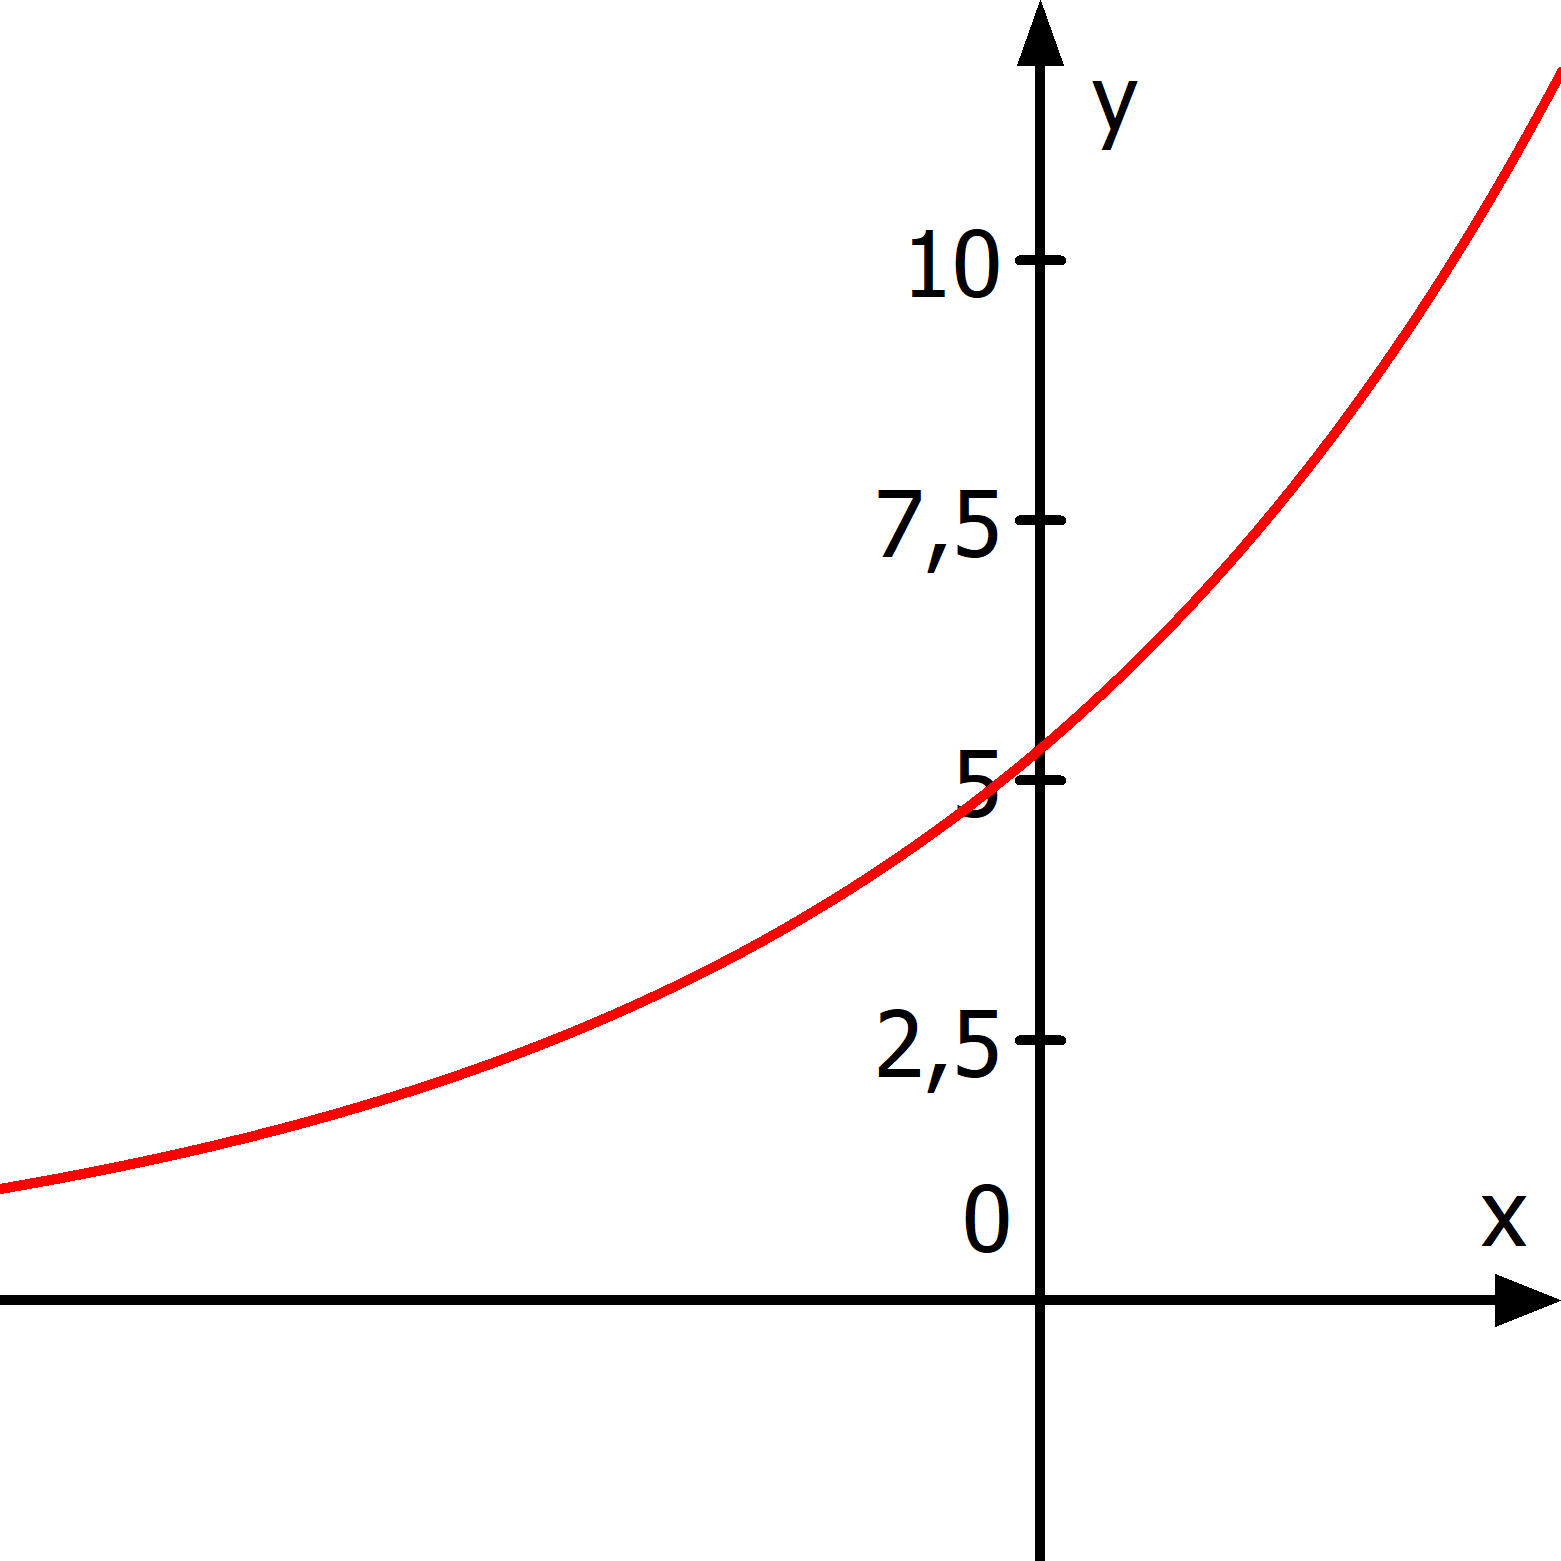
\includegraphics[width=.6\linewidth]{\eFkt/pics/A1p.png}
				\item \(f(x)=-\frac{1}{4}e^{-\frac{2}{3}x}\)

				Asymptote \(y=0\)

				y-Achsenabschnitt: \(f(0)=-\frac{1}{4}\)

				Monoton wachsend

				\(f(x)\xrightarrow{\hphantom{\ }x\to-\infty\hphantom{\ }}-\infty\)

				\(f(x)\xrightarrow{\hphantom{\ }x\to\infty\hphantom{\ }}0\)

				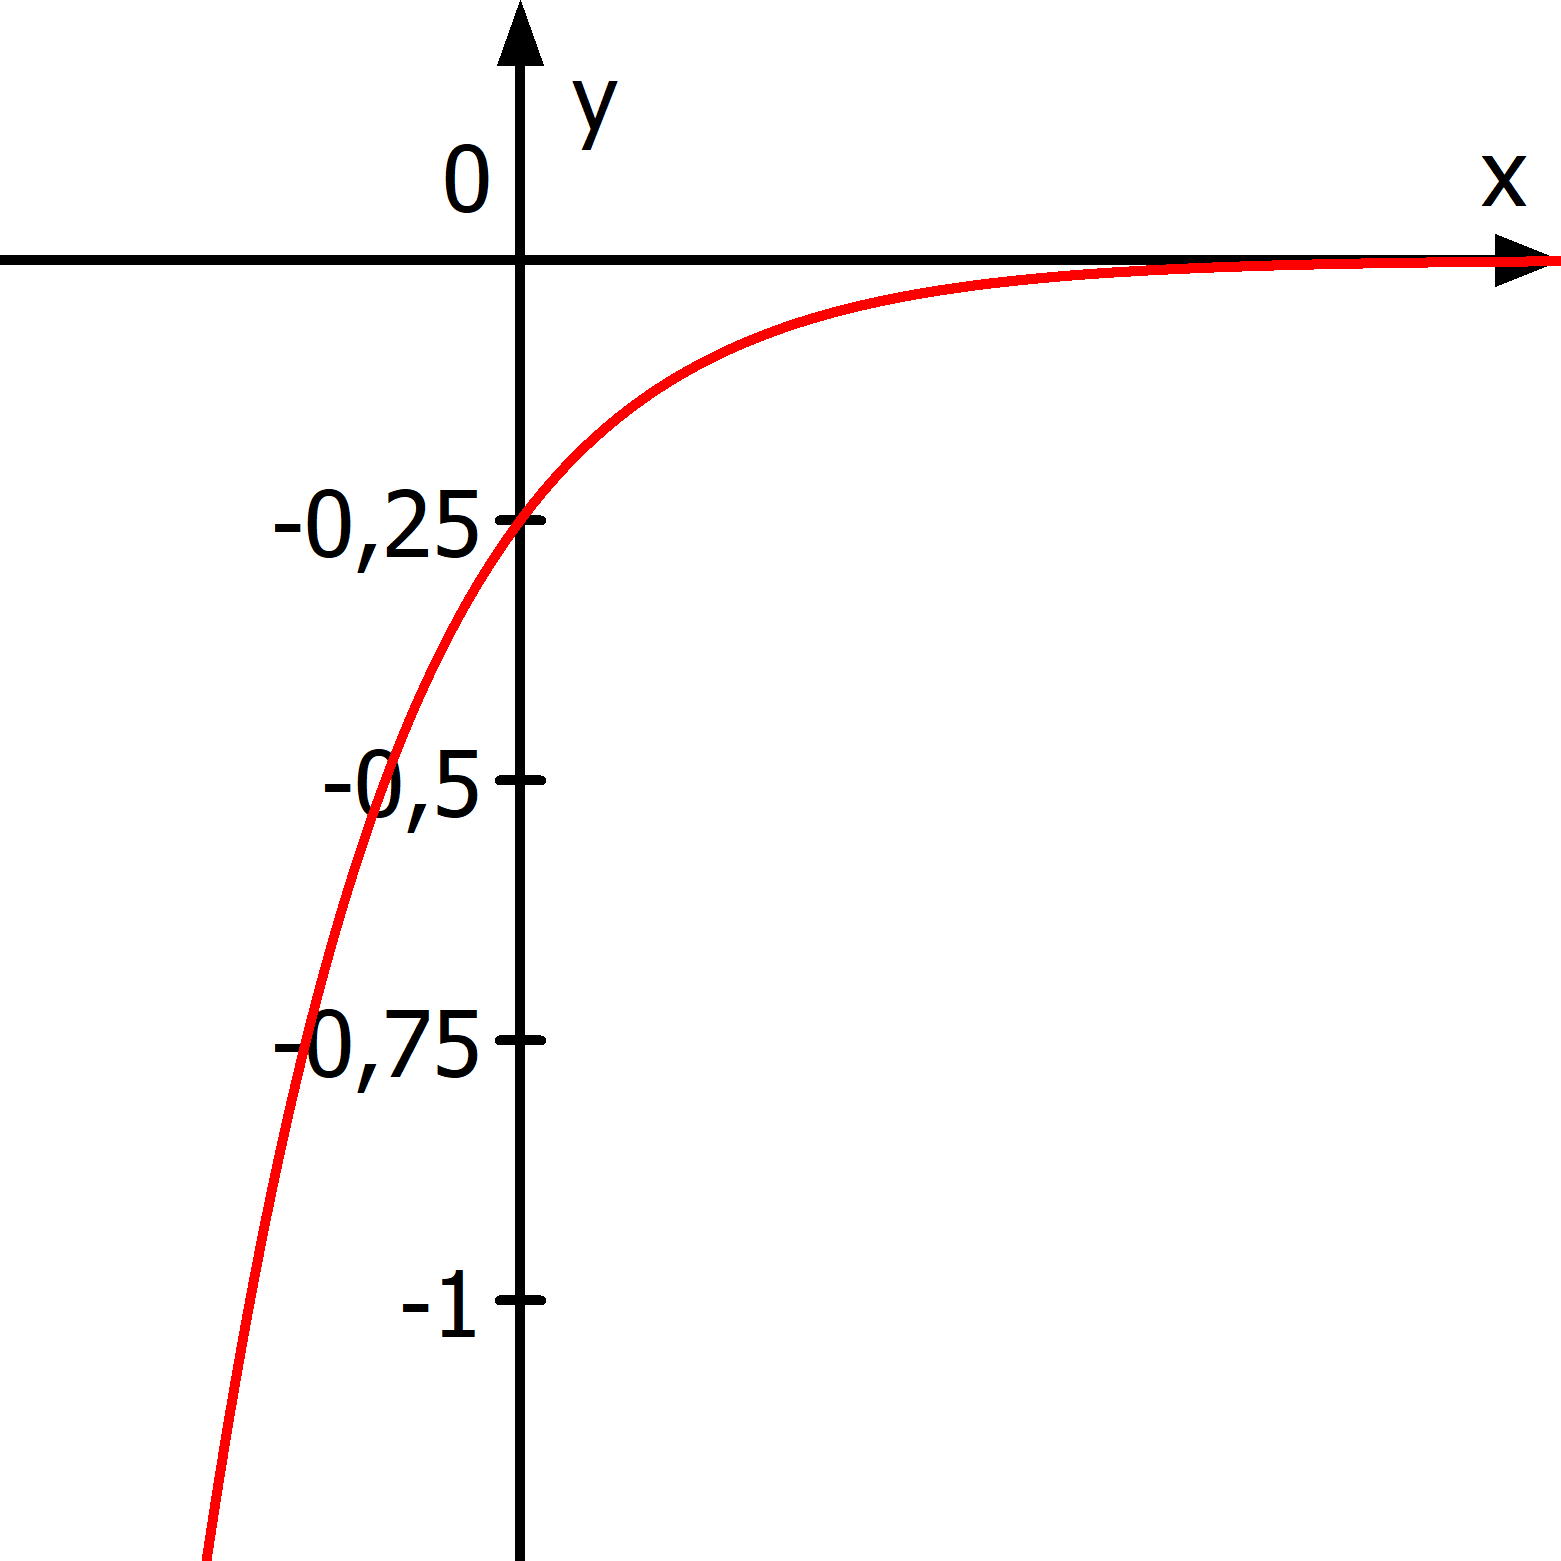
\includegraphics[width=.6\linewidth]{\eFkt/pics/A1q.png}
				\item \(f(x)=-2e^{0,2x}\)

				Asymptote \(y=0\)

				y-Achsenabschnitt: \(f(0)=-2\)

				Monoton fallend

				\(f(x)\xrightarrow{\hphantom{\ }x\to-\infty\hphantom{\ }}0\)

				\(f(x)\xrightarrow{\hphantom{\ }x\to\infty\hphantom{\ }}-\infty\)

				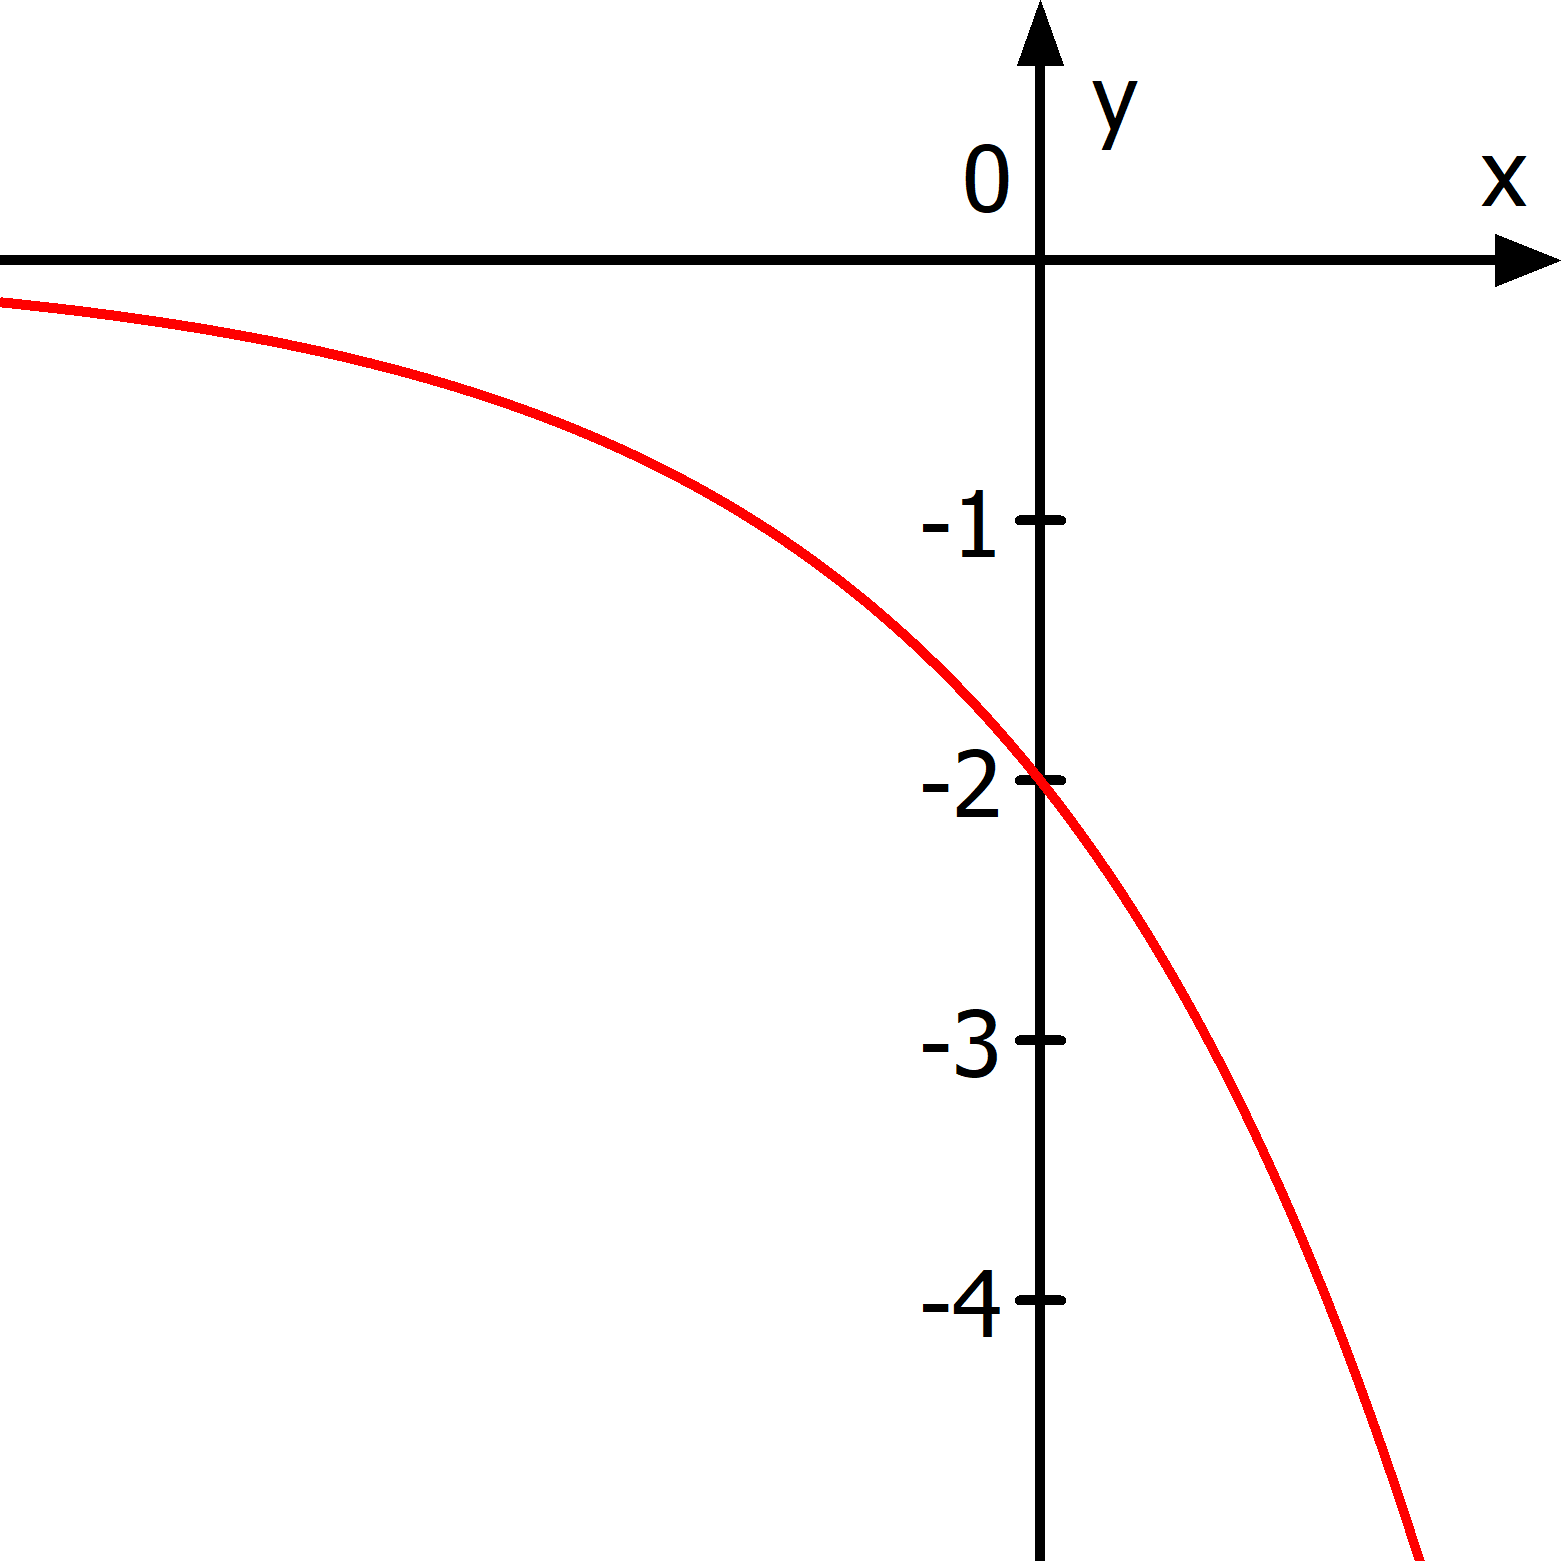
\includegraphics[width=.6\linewidth]{\eFkt/pics/A1r.png}
			\end{enumerate}
		\end{minipage}}%
	\end{minipage}%

	%%%%% s bis x
	\begin{minipage}{\textwidth}
		\adjustbox{valign=t}{\begin{minipage}{0.5\textwidth}
			\begin{enumerate}[label=\alph*)]
				\setcounter{enumi}{18}
				\item \(f(x)=1,8e^{-4x}\)

				Asymptote \(y=0\)

				y-Achsenabschnitt: \(f(0)=1,8\)

				Monoton fallend

				\(f(x)\xrightarrow{\hphantom{\ }x\to-\infty\hphantom{\ }}\infty\)

				\(f(x)\xrightarrow{\hphantom{\ }x\to\infty\hphantom{\ }}0\)

				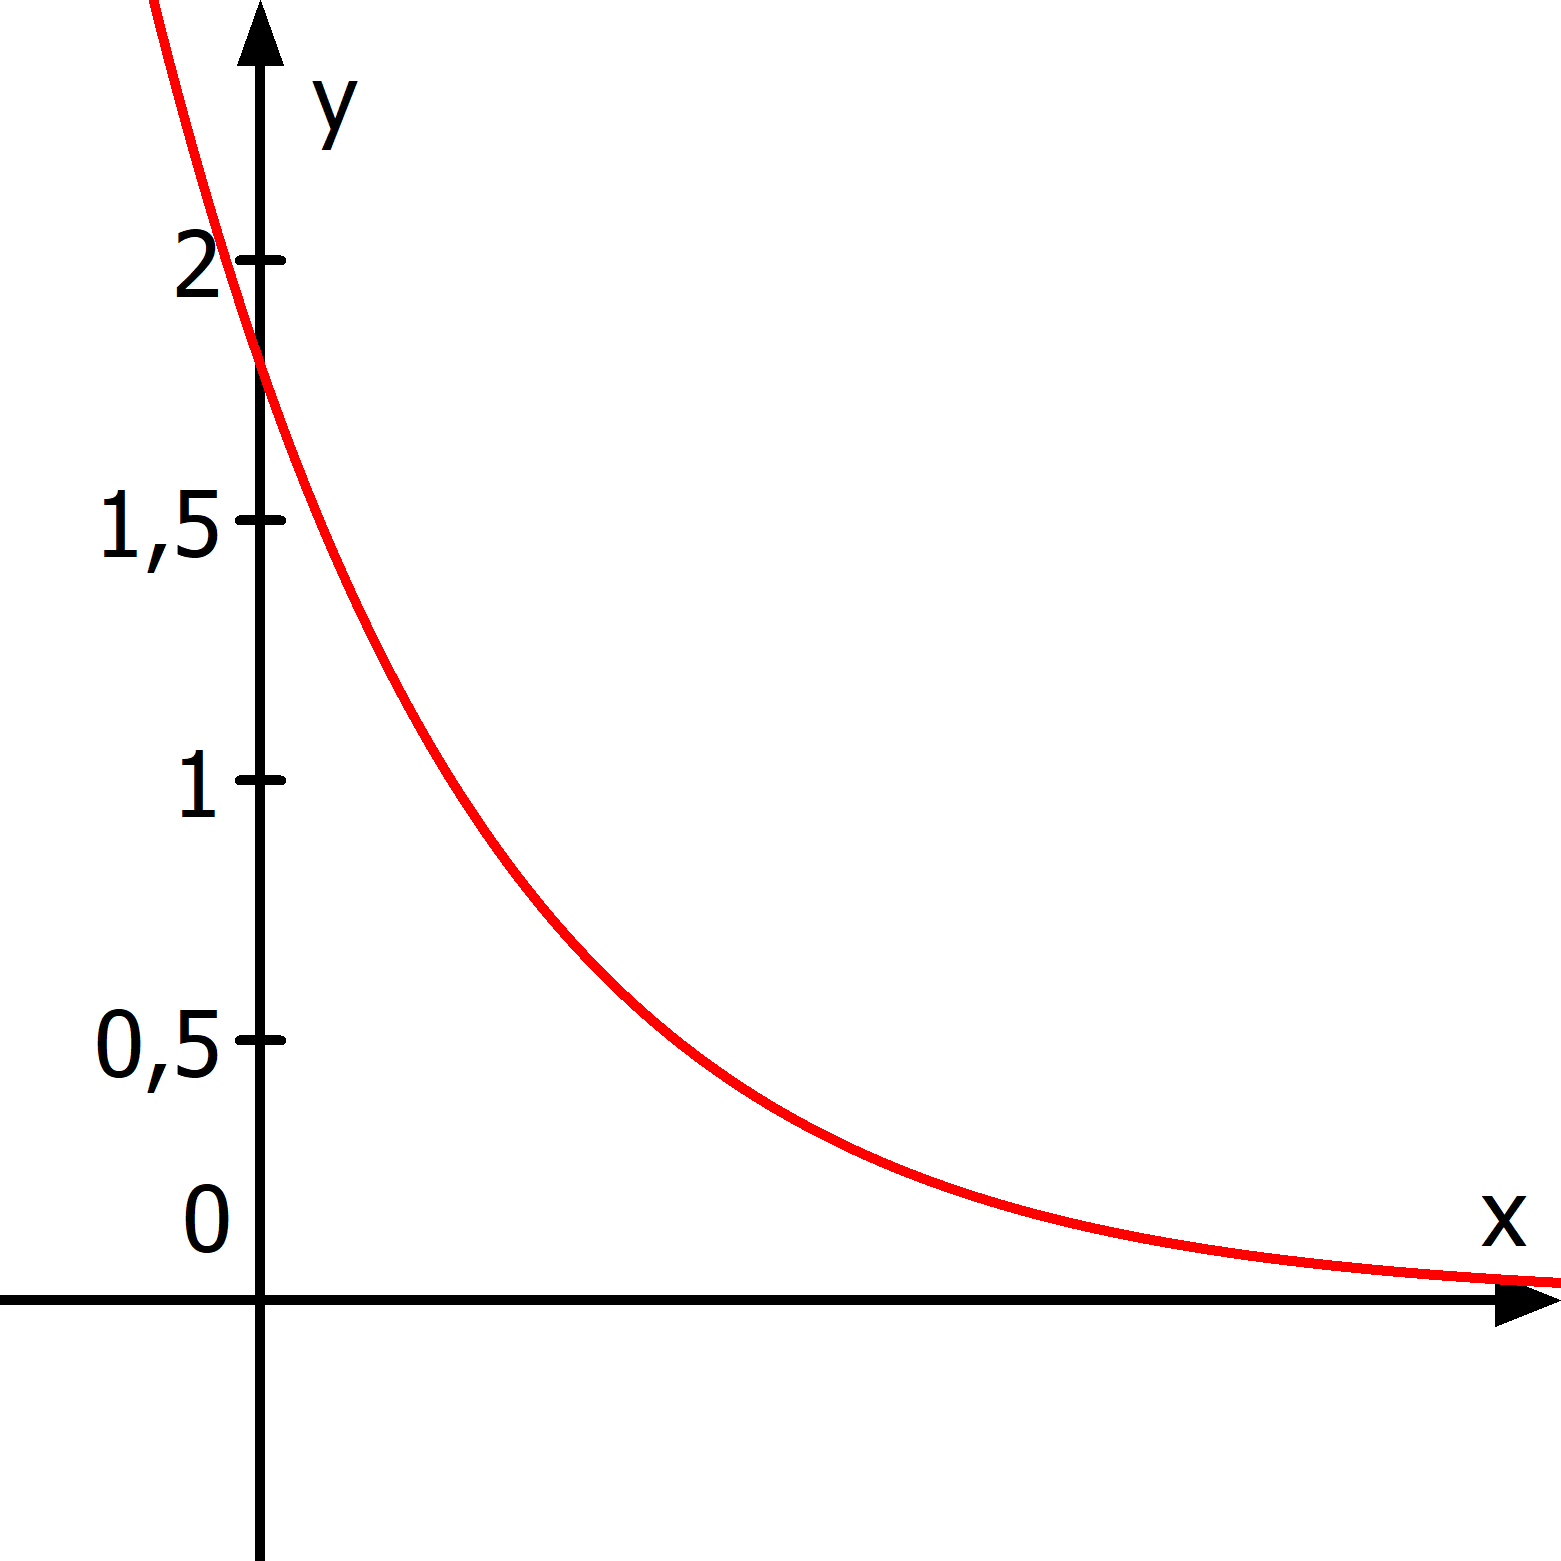
\includegraphics[width=.6\linewidth]{\eFkt/pics/A1s.png}
				\item \(f(x)=5e^{7x}\)

				Asymptote \(y=0\)

				y-Achsenabschnitt: \(f(0)=5\)

				Monoton wachsend

				\(f(x)\xrightarrow{\hphantom{\ }x\to-\infty\hphantom{\ }}0\)

				\(f(x)\xrightarrow{\hphantom{\ }x\to\infty\hphantom{\ }}\infty\)

				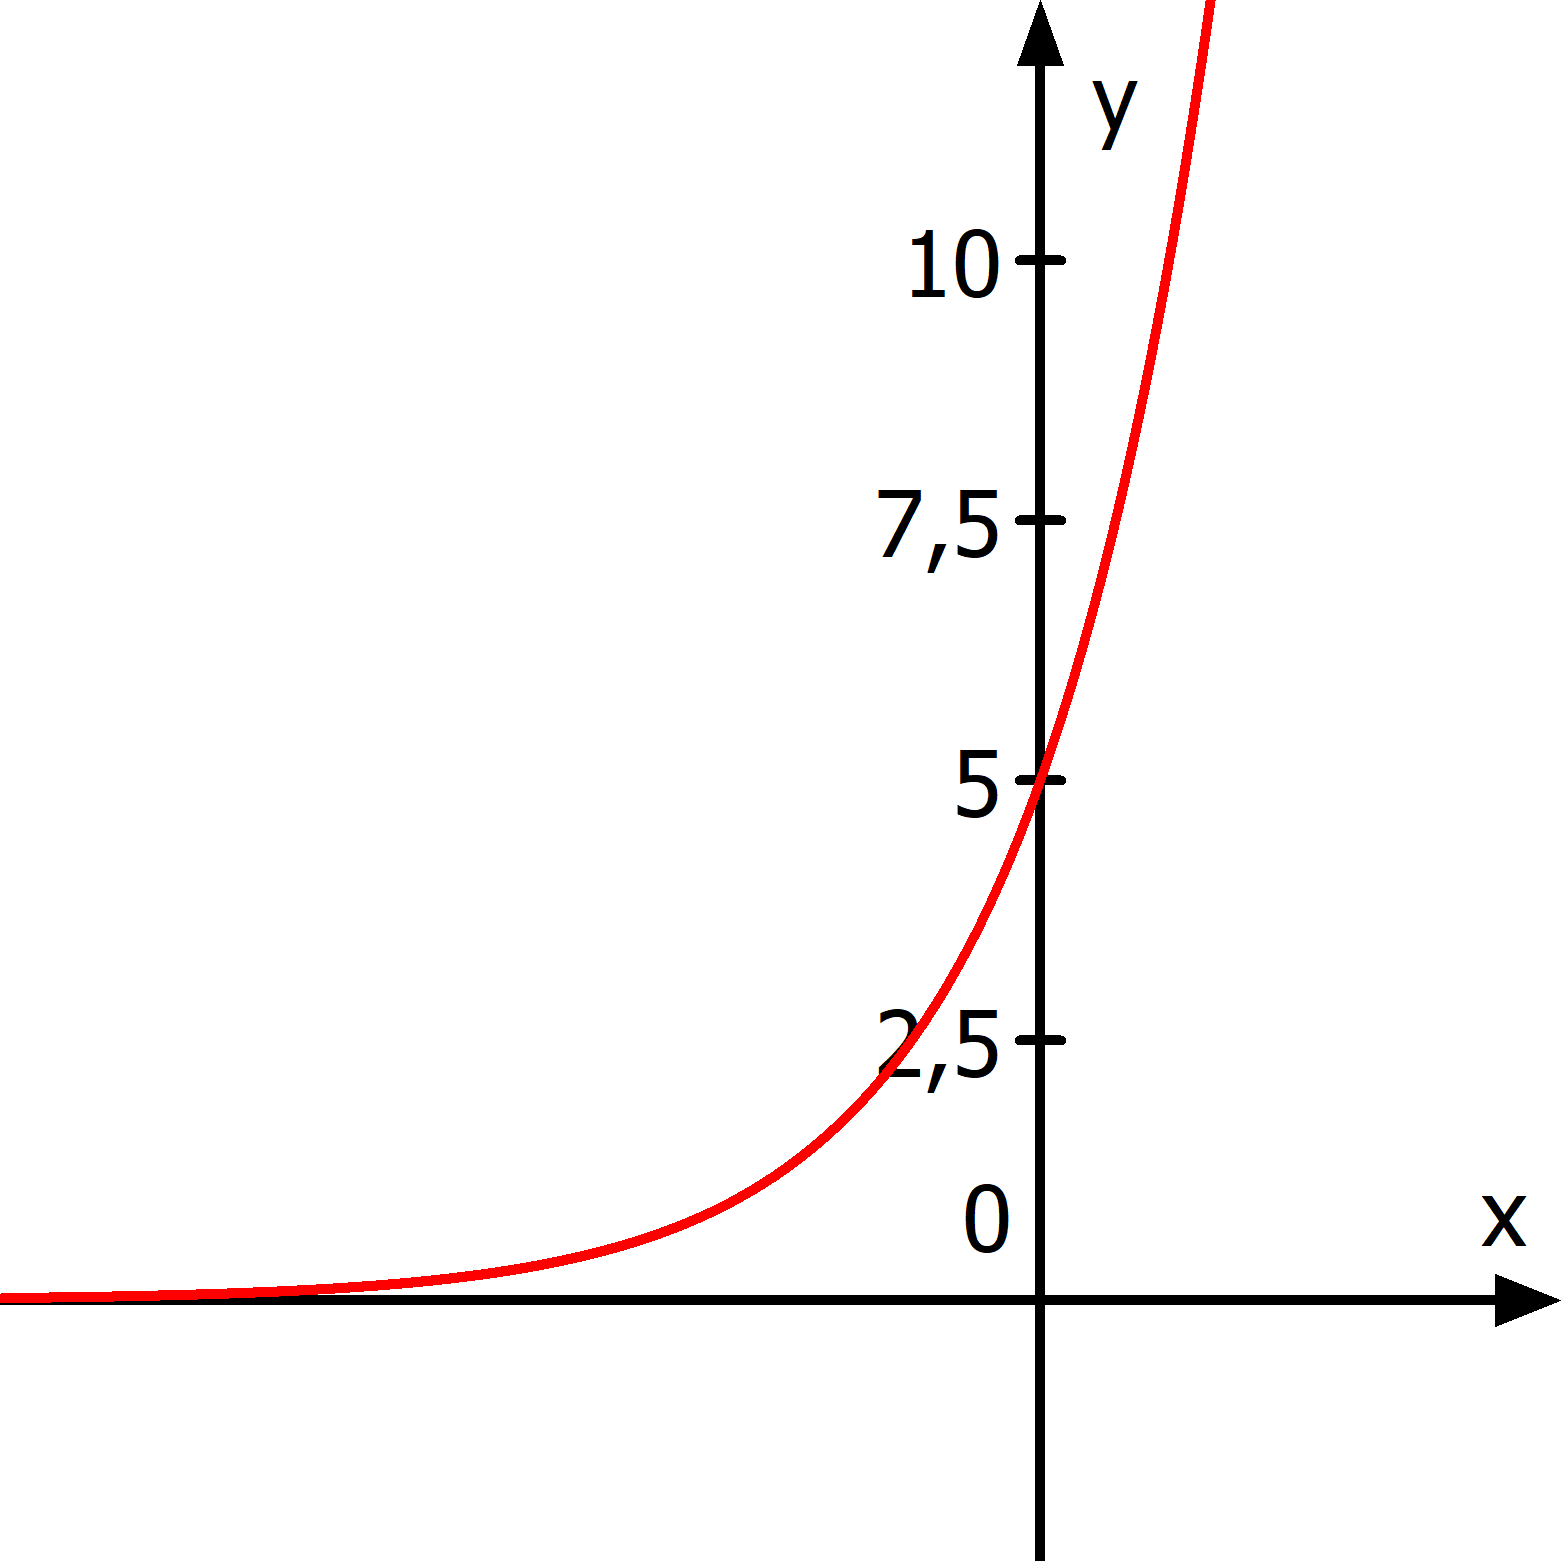
\includegraphics[width=.6\linewidth]{\eFkt/pics/A1t.png}
				\item \(f(x)=-\frac{8}{3}e^{\frac{3}{8}x}\)

				Asymptote \(y=0\)

				y-Achsenabschnitt: \(f(0)=-\frac{8}{3}\)

				Monoton fallend

				\(f(x)\xrightarrow{\hphantom{\ }x\to-\infty\hphantom{\ }}0\)

				\(f(x)\xrightarrow{\hphantom{\ }x\to\infty\hphantom{\ }}-\infty\)

				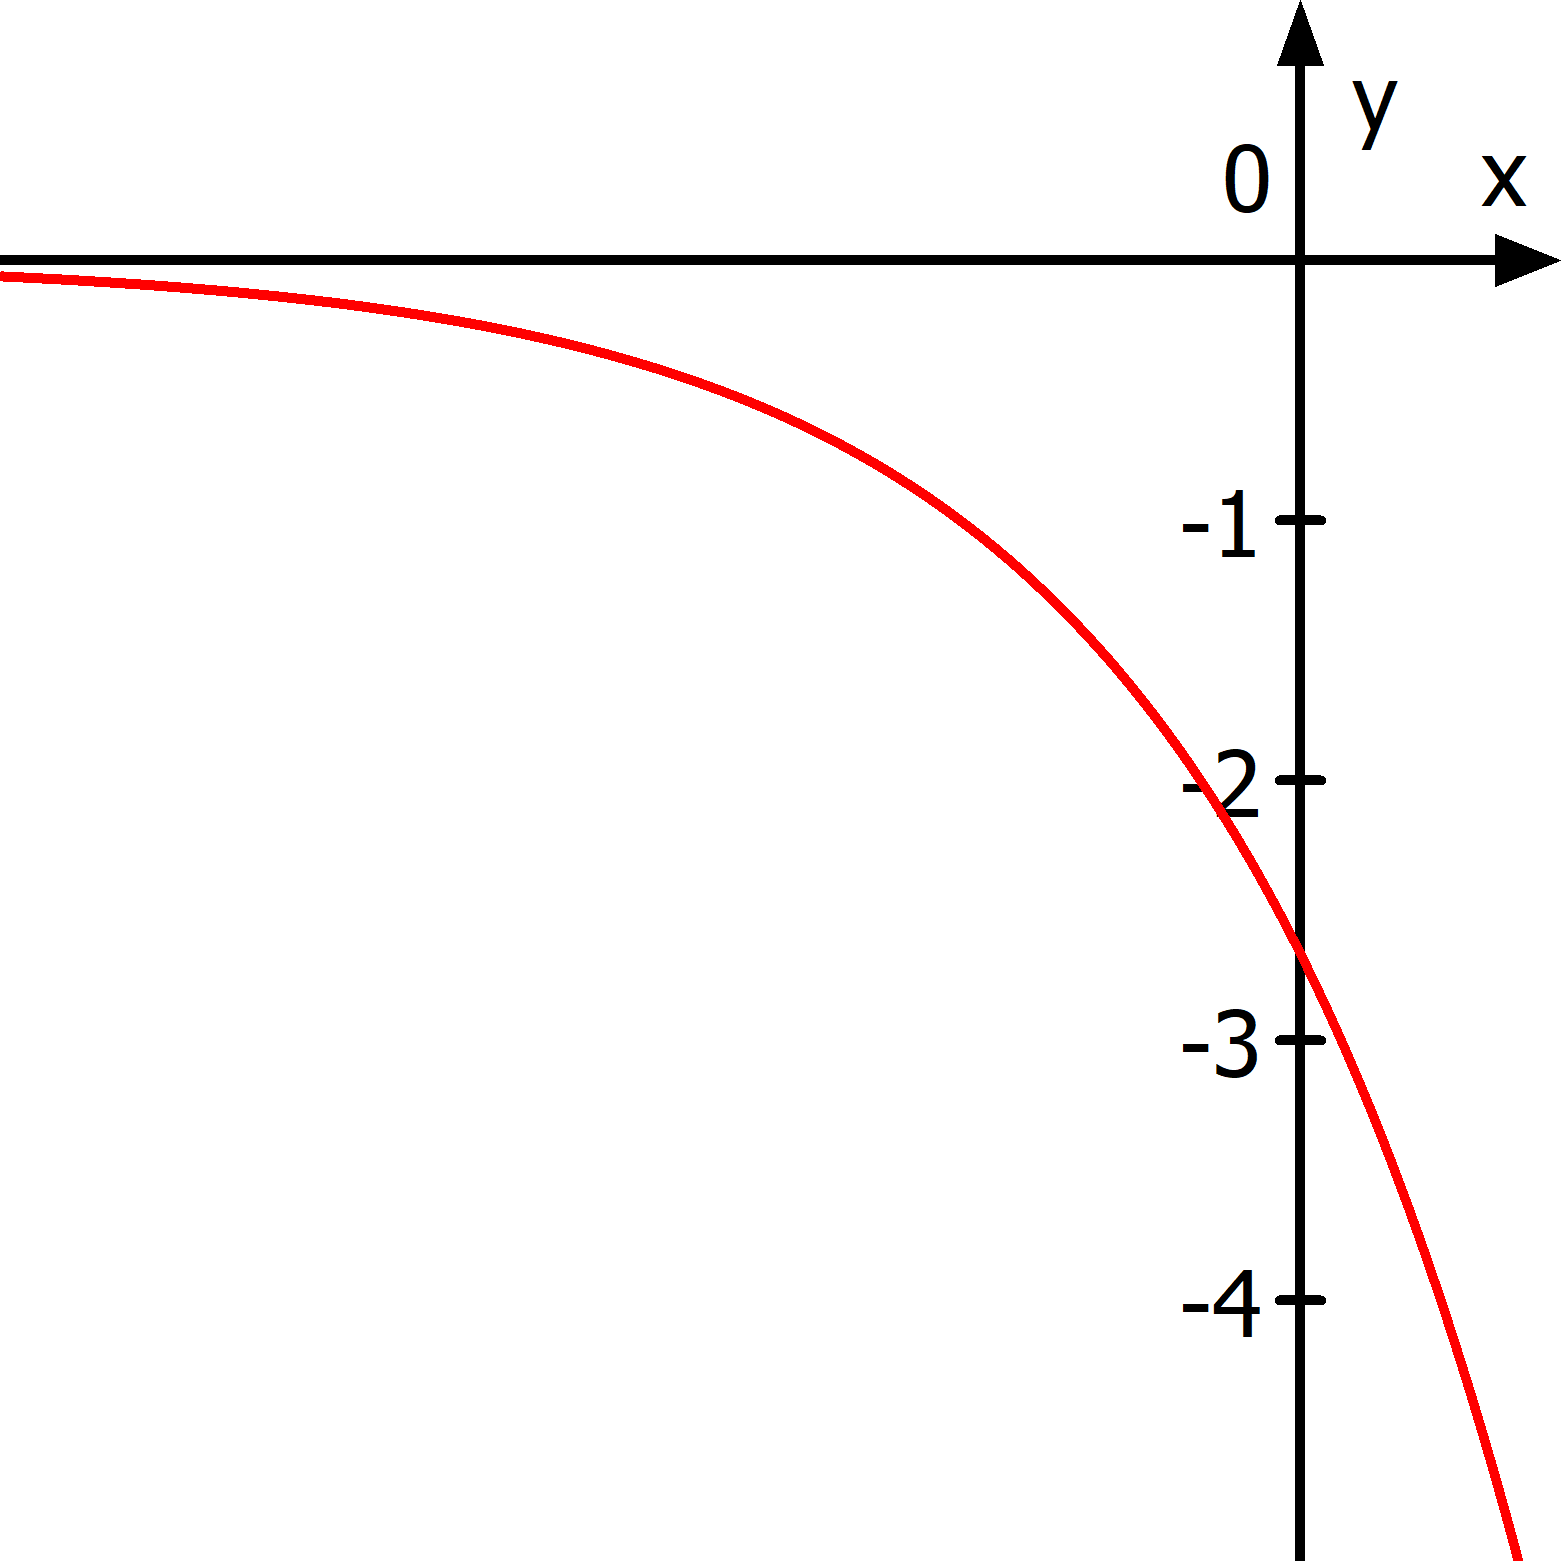
\includegraphics[width=.6\linewidth]{\eFkt/pics/A1u.png}
			\end{enumerate}
		\end{minipage}}%
		\adjustbox{valign=t}{\begin{minipage}{0.5\textwidth}
			\begin{enumerate}[label=\alph*)]
				\setcounter{enumi}{21}
				\item \(f(x)=-0,1^{-0,3x}\)

				Asymptote \(y=0\)

				y-Achsenabschnitt: \(f(0)=-0,1\)

				Monoton wachsend

				\(f(x)\xrightarrow{\hphantom{\ }x\to-\infty\hphantom{\ }}-\infty\)

				\(f(x)\xrightarrow{\hphantom{\ }x\to\infty\hphantom{\ }}0\)

				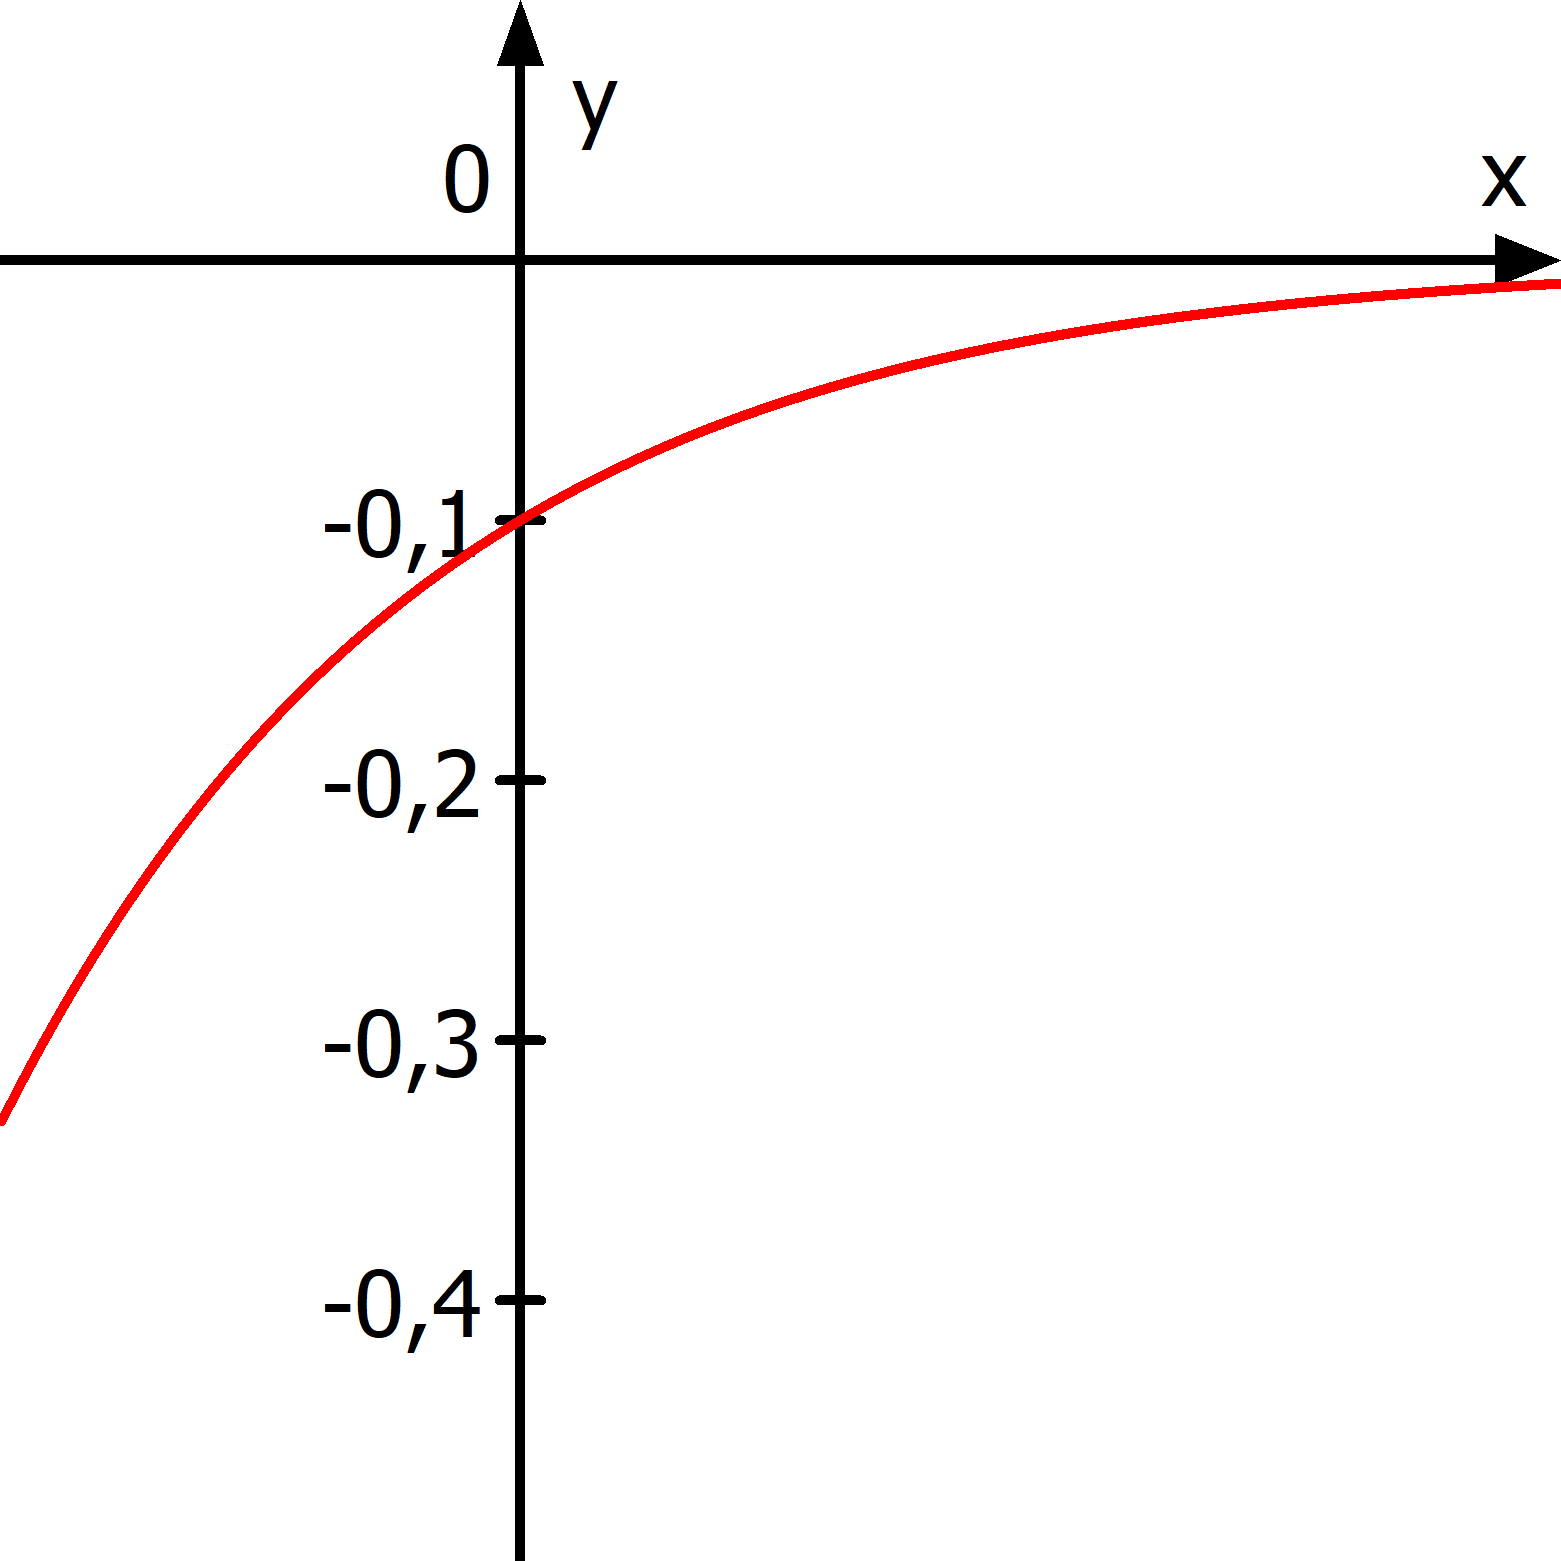
\includegraphics[width=.6\linewidth]{\eFkt/pics/A1v.png}
				\item \(f(x)=10e^{-4x}\)

				Asymptote \(y=0\)

				y-Achsenabschnitt: \(f(0)=10\)

				Monoton fallend

				\(f(x)\xrightarrow{\hphantom{\ }x\to-\infty\hphantom{\ }}\infty\)

				\(f(x)\xrightarrow{\hphantom{\ }x\to\infty\hphantom{\ }}0\)

				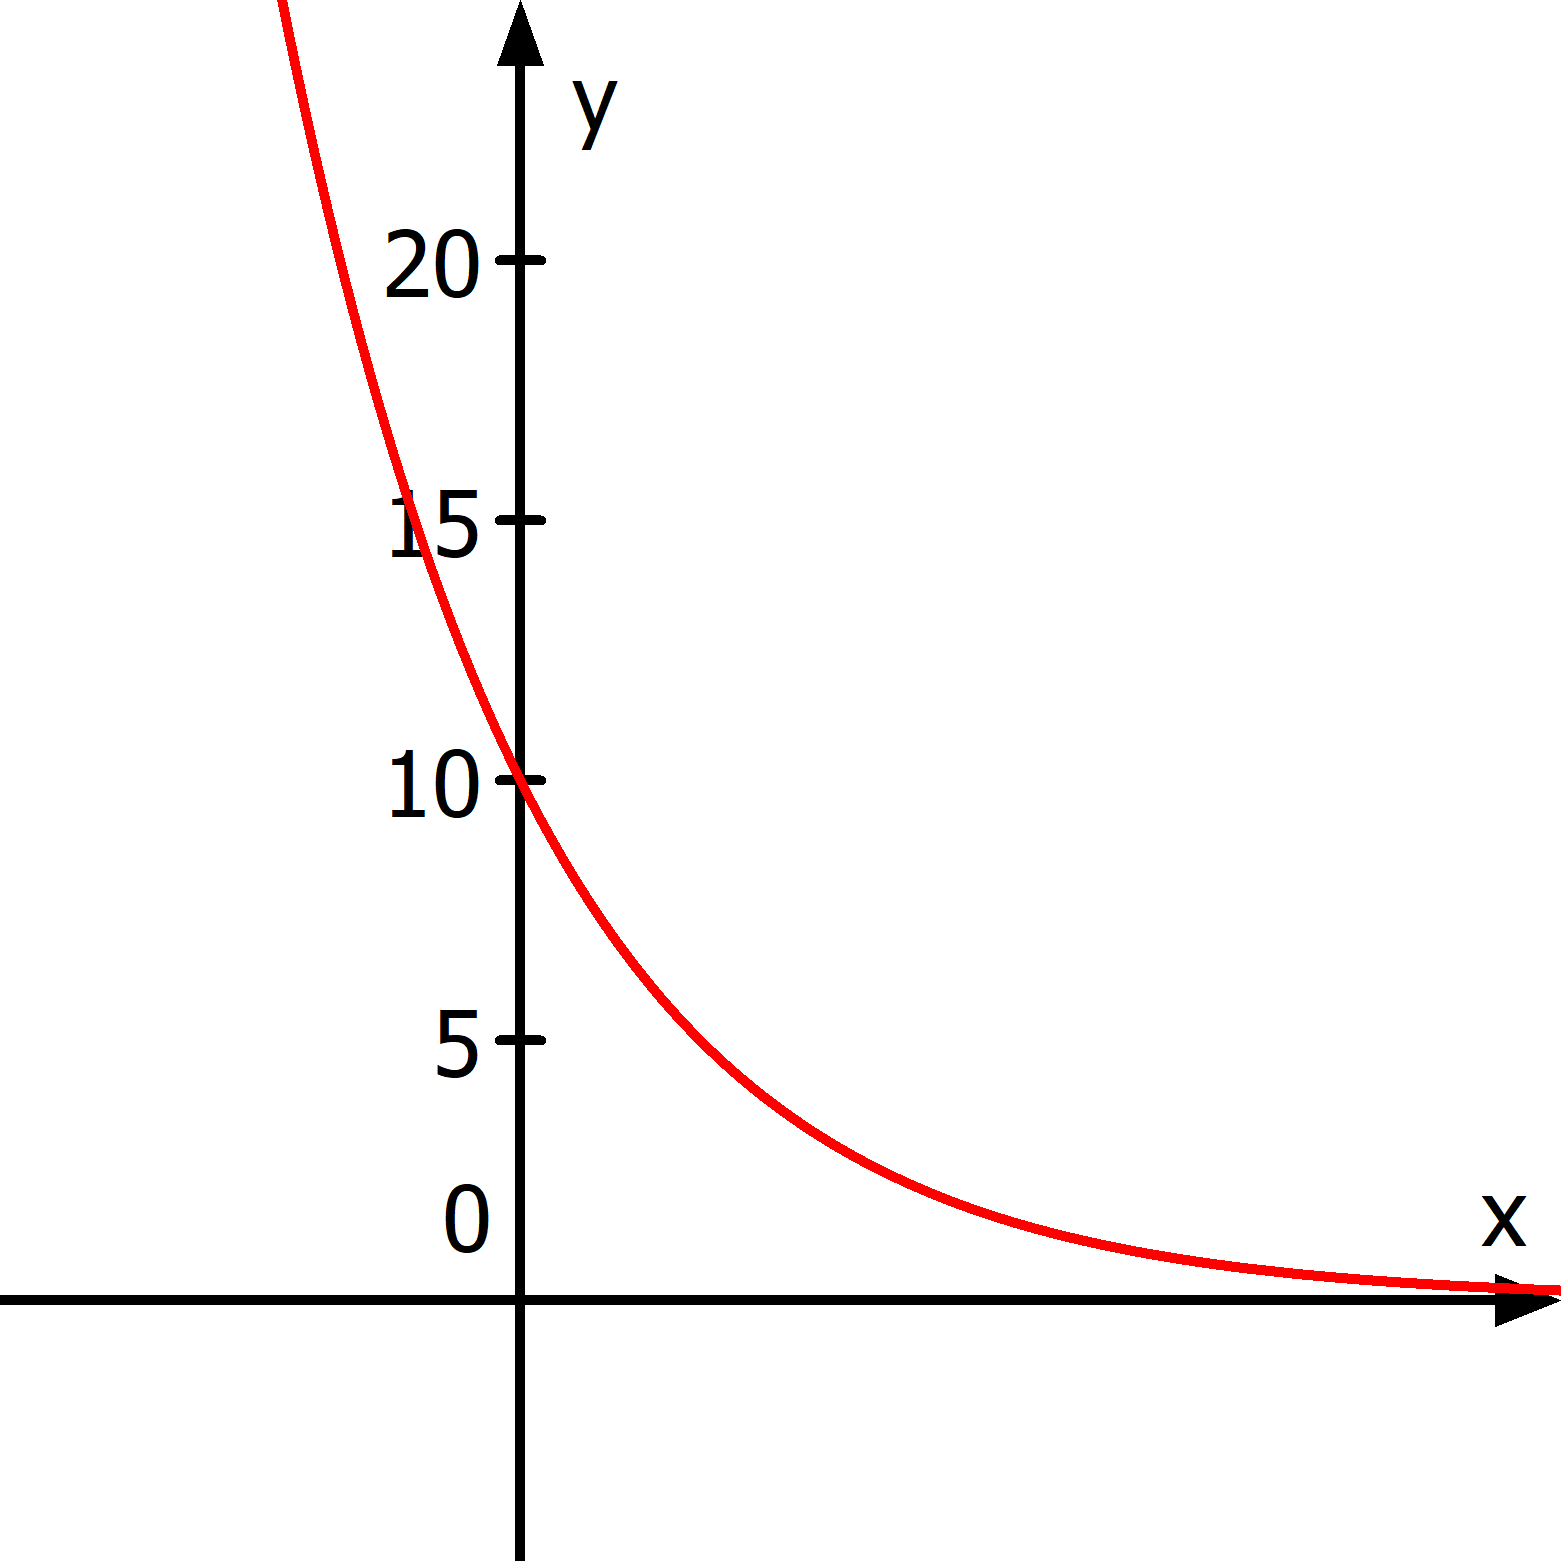
\includegraphics[width=.6\linewidth]{\eFkt/pics/A1w.png}
				\item \(f(x)=-5e^{6x}\)

				Asymptote \(y=0\)

				y-Achsenabschnitt: \(f(0)=-5\)

				Monoton fallend

				\(f(x)\xrightarrow{\hphantom{\ }x\to-\infty\hphantom{\ }}0\)

				\(f(x)\xrightarrow{\hphantom{\ }x\to\infty\hphantom{\ }}-\infty\)

				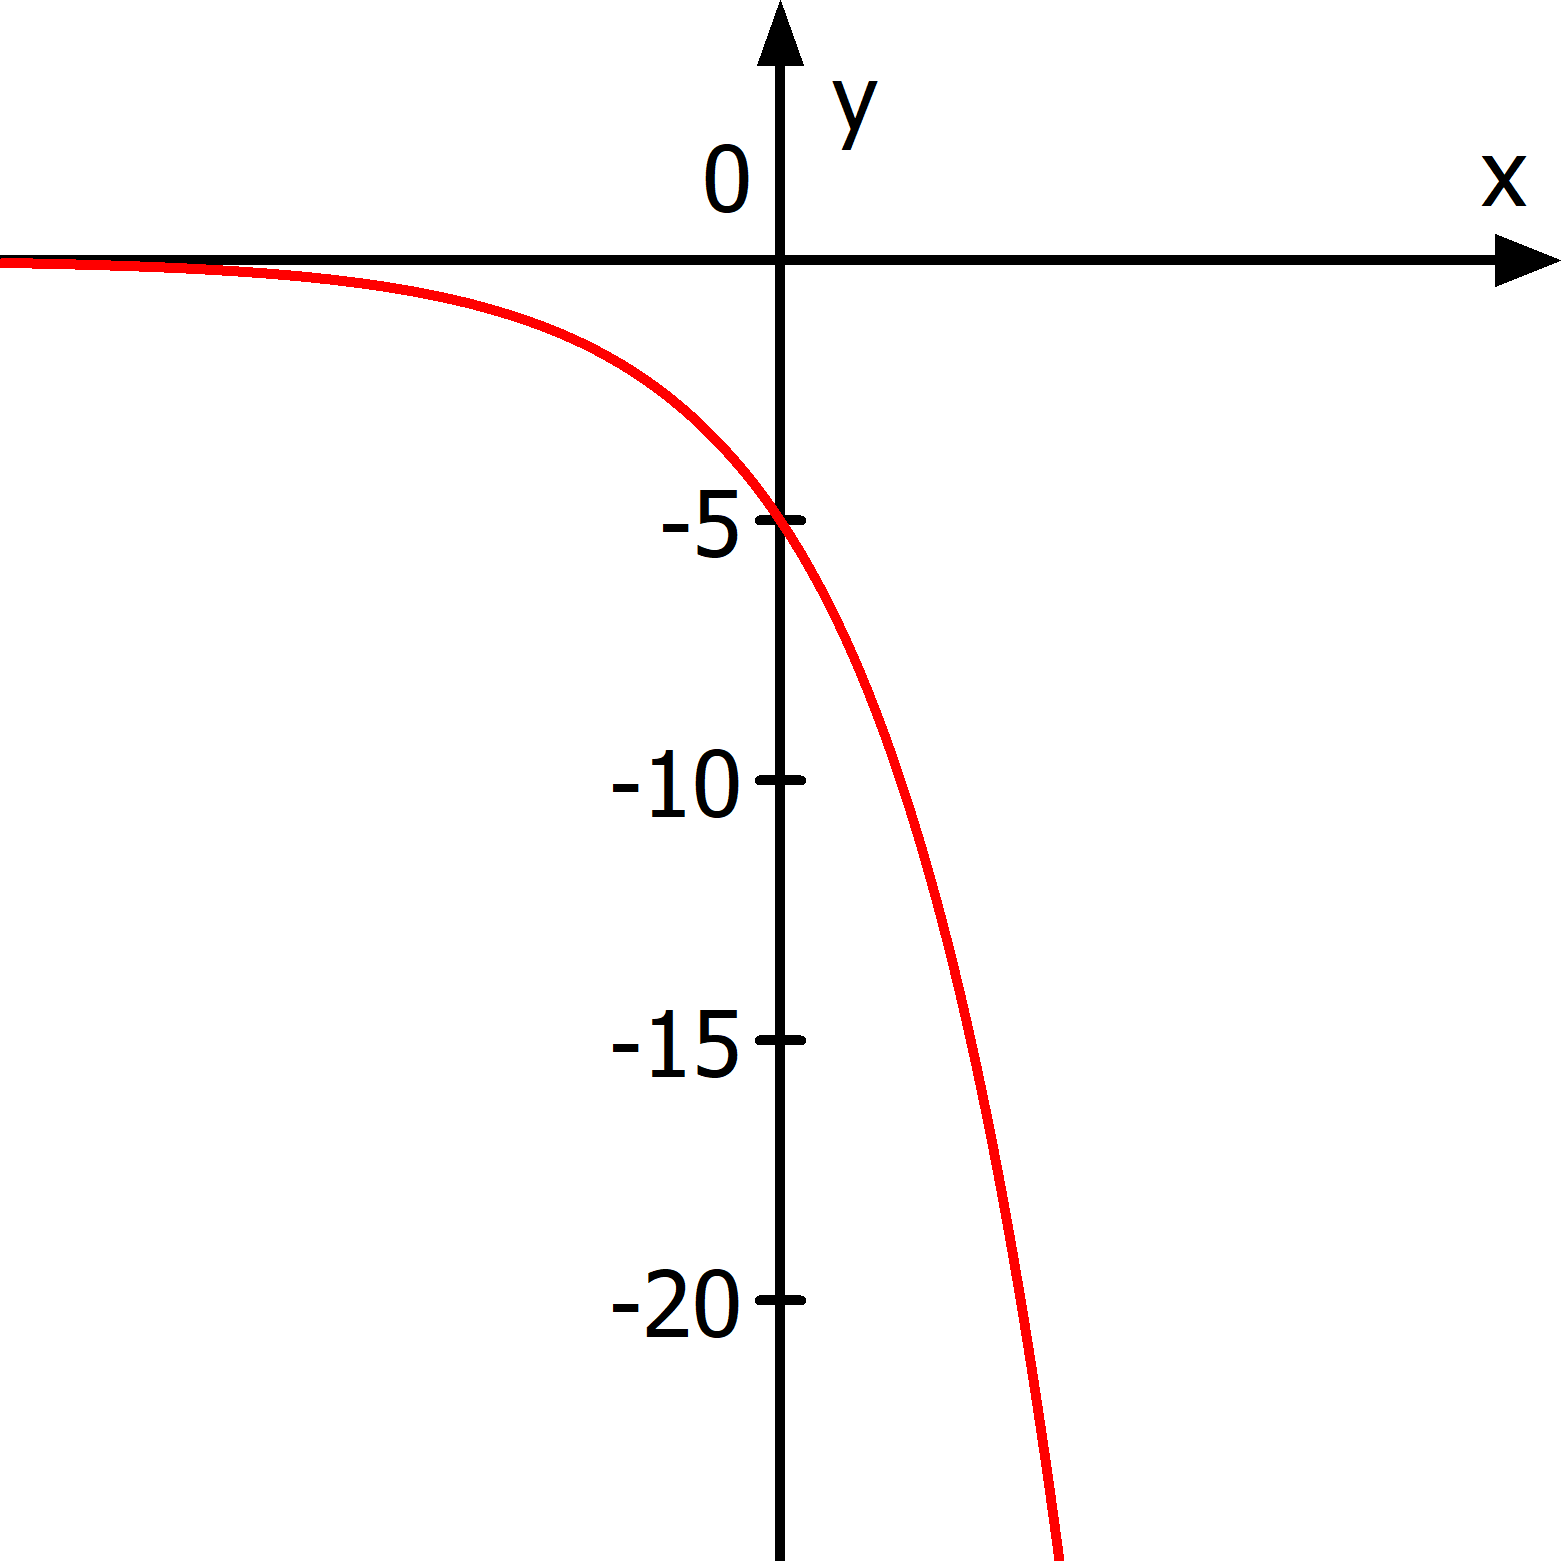
\includegraphics[width=.6\linewidth]{\eFkt/pics/A1x.png}
			\end{enumerate}
		\end{minipage}}%
	\end{minipage}%

	%%%%% y bis z
	\begin{minipage}{\textwidth}
		\adjustbox{valign=t}{\begin{minipage}{0.5\textwidth}
			\begin{enumerate}[label=\alph*)]
				\setcounter{enumi}{24}
				\item \(f(x)=-0,9e^{-1,1x}\)

				Asymptote \(y=0\)

				y-Achsenabschnitt: \(f(0)=-0,9\)

				Monoton wachsend

				\(f(x)\xrightarrow{\hphantom{\ }x\to-\infty\hphantom{\ }}-\infty\)

				\(f(x)\xrightarrow{\hphantom{\ }x\to\infty\hphantom{\ }}0\)

				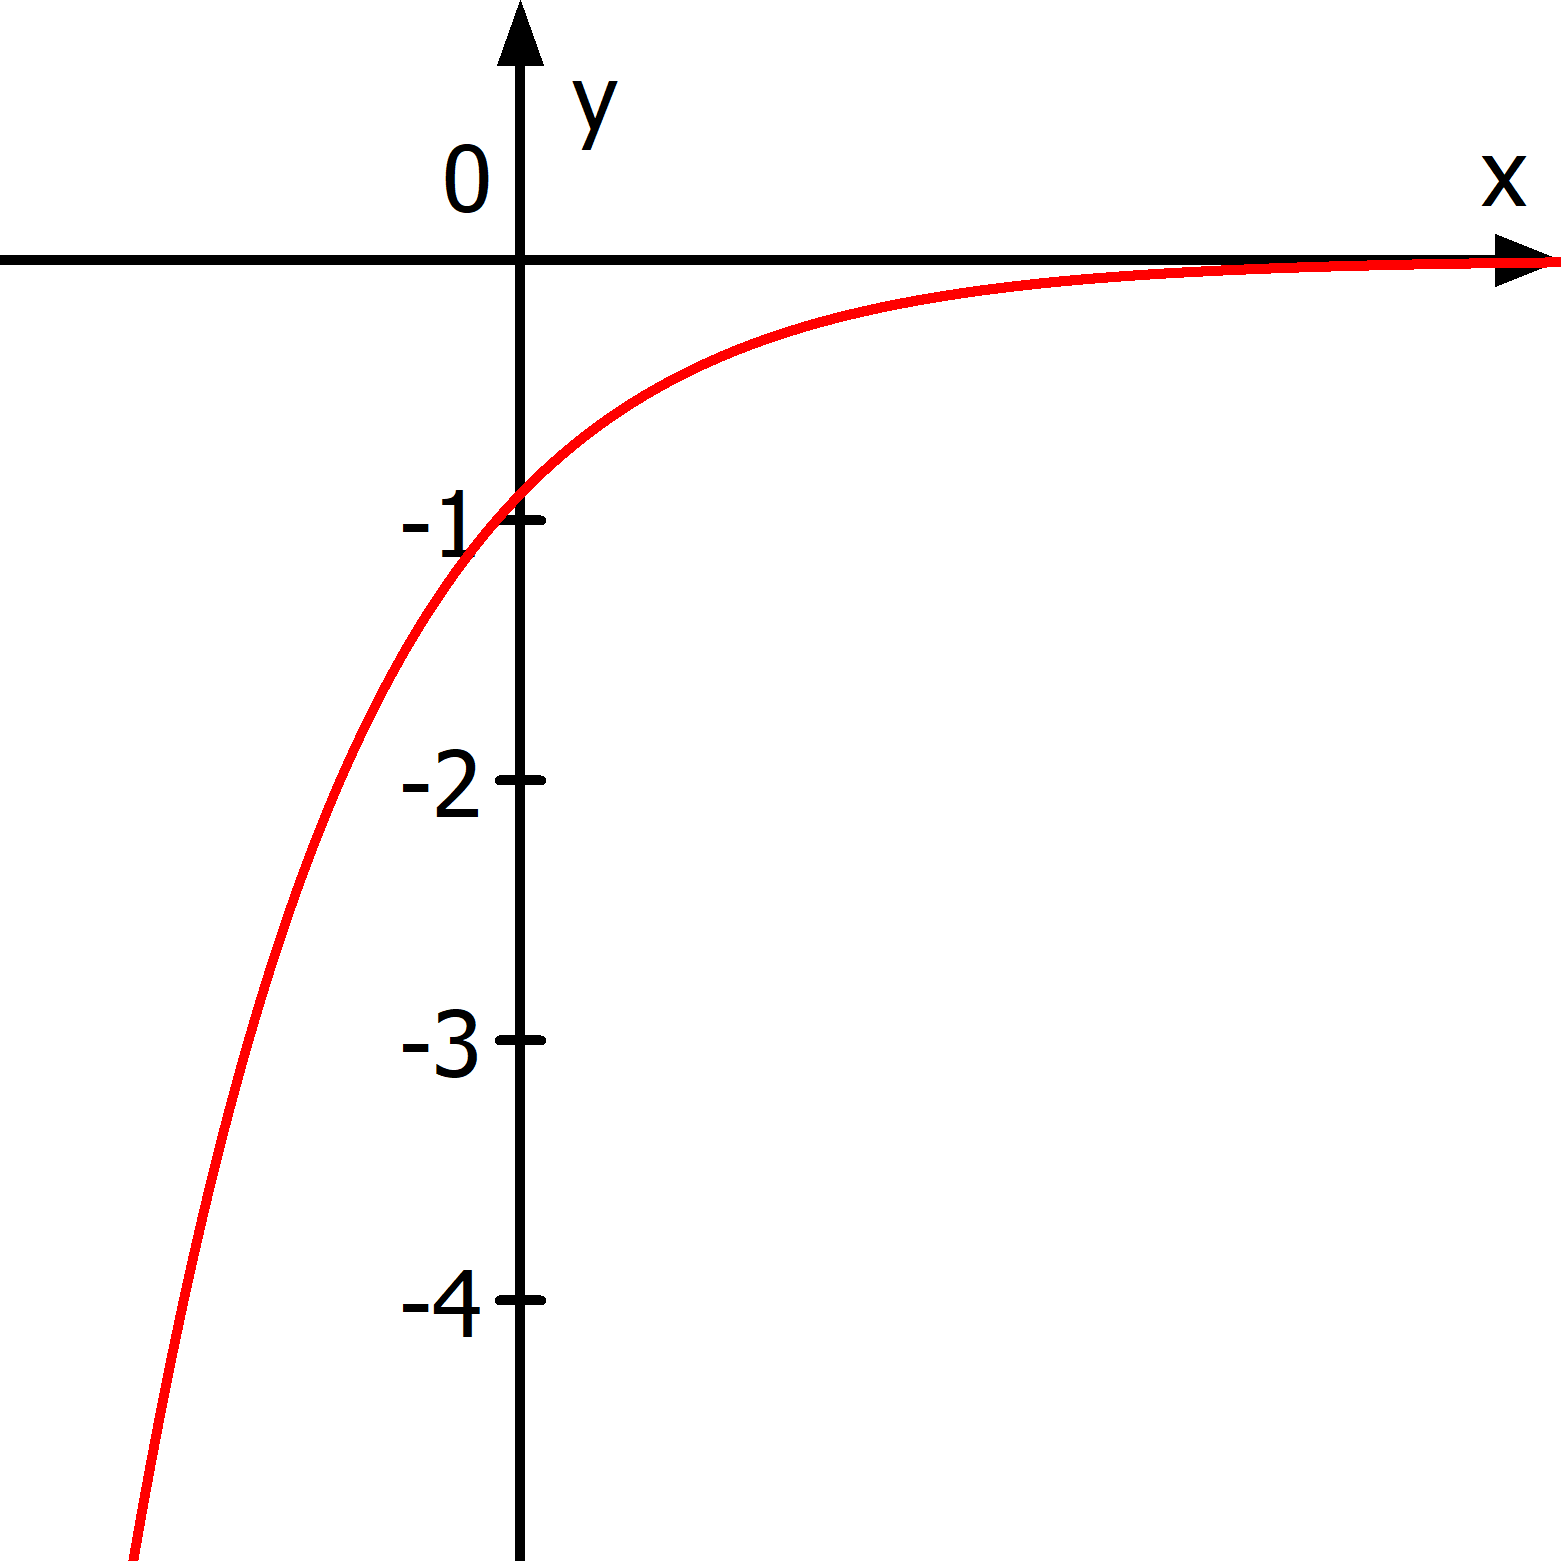
\includegraphics[width=.6\linewidth]{\eFkt/pics/A1y.png}
			\end{enumerate}
		\end{minipage}}%
		\adjustbox{valign=t}{\begin{minipage}{0.5\textwidth}
			\begin{enumerate}[label=\alph*)]
				\setcounter{enumi}{25}
				\item \(f(x)=\frac{11}{6}e^{\frac{8}{7}x}\)

				Asymptote \(y=0\)

				y-Achsenabschnitt: \(f(0)=\frac{11}{6}\)

				Monoton wachsend

				\(f(x)\xrightarrow{\hphantom{\ }x\to-\infty\hphantom{\ }}0\)

				\(f(x)\xrightarrow{\hphantom{\ }x\to\infty\hphantom{\ }}\infty\)

				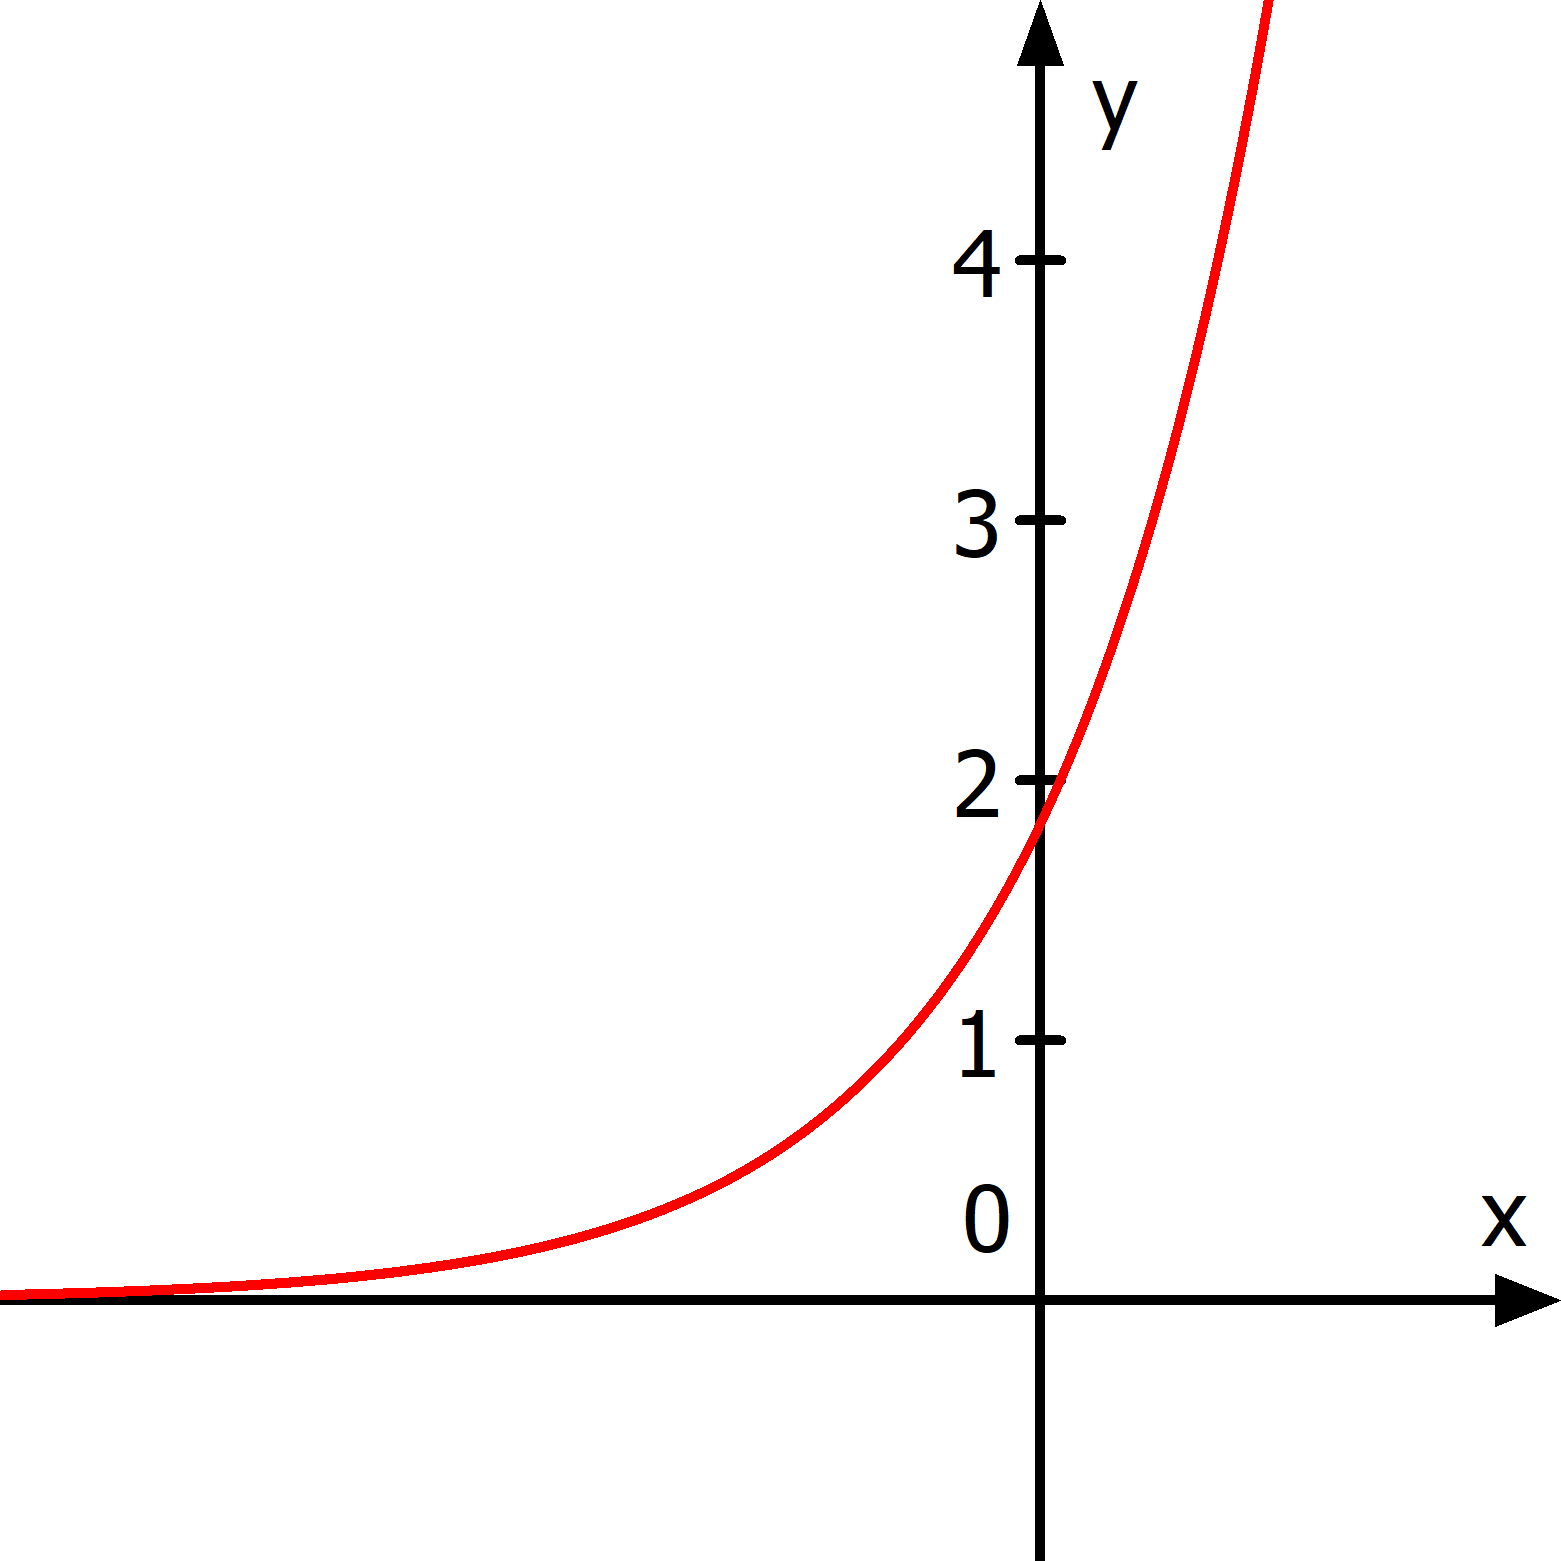
\includegraphics[width=.6\linewidth]{\eFkt/pics/A1z.png}
			\end{enumerate}
		\end{minipage}}%
	\end{minipage}%
\end{Answer}